\documentclass[a4paper, openany, 12pt]{article}

%% подключаем стандарт библиографии
\bibliographystyle{gost71u}

%% для "Abstract" в классе book
% \newenvironment{abstract}{}{}
% \usepackage{abstract}

%% подключаем преамбулу: в ней содержится подключение всех необходимых пакетов
%% Работа с русским языком
\usepackage{cmap}			 % поиск в PDF
\usepackage{mathtext} 		 % русские буквы в формулах
\usepackage[T2A]{fontenc}	 % кодировка
\usepackage[utf8]{inputenc}	 % кодировка исходного текста
\usepackage[russian]{babel}	 % локализация и переносы

%% Пакеты для работы с математикой
\usepackage{amsmath,amsfonts,amssymb,amsthm,mathtools}
\usepackage{icomma}

%% Нумерация формул (опционально)
%\mathtoolsset{showonlyrefs=true} % показывать номера только у тех формул, на которые есть \eqref{} в тексте.
%\usepackage{leqno}               % нумерация формул слева

%% Шрифты
\usepackage{euscript}	 % шрифт "Евклид"
\usepackage{mathrsfs}    % красивый мат. шрифт

%% Некоторые полезные макросы для дебага (в случае недоверия авторам шаблона)
\makeatletter
\newcommand\thefontsize{The current font size is: \f@size pt} % пример: \section{\thefontsize}
\makeatother

%% Настройка размеров шрифтов
\makeatletter
\renewcommand\Huge{\@setfontsize\Huge{14pt}{1.5}}
\renewcommand\huge{\@setfontsize\huge{14pt}{1.5}}
\renewcommand\Large{\@setfontsize\Large{14pt}{1.5}}
\renewcommand\large{\@setfontsize\large{12pt}{1.5}}
\makeatother

%% Поля (геометрия страницы)
\usepackage[left=3cm,right=1.5cm,top=2cm,bottom=2cm,bindingoffset=0cm]{geometry}

%% Русские списки
\usepackage{enumitem}
\makeatletter
\AddEnumerateCounter{\asbuk}{\russian@alph}{щ}
\makeatother

%% Работа с картинками
\usepackage{caption}
\captionsetup{justification=centering} % центрирование подписей к картинкам
\usepackage{graphicx}                  % вставки рисунков
\graphicspath{{images/}{images2/}}     % папки с картинками
\setlength\fboxsep{3pt}                % отступ рамки \fbox{} от рисунка
\setlength\fboxrule{1pt}               % толщина линий рамки \fbox{}
\usepackage{wrapfig}                   % обтекание рисунков и таблиц текстом

%% Работа с таблицами
\usepackage{array,tabularx,tabulary,booktabs} % дополнительная работа с таблицами
\usepackage{longtable}                        % длинные таблицы
\usepackage{multirow}                         % слияние строк в таблице

%% Красная строка
\setlength{\parindent}{2em}

%% Интервалы
\linespread{1}
\usepackage{multirow}

%% TikZ
\usepackage{tikz}
\usetikzlibrary{graphs,graphs.standard}

%% Верхний колонтитул
\usepackage{fancyhdr}
\pagestyle{fancy}

%% Перенос знаков в формулах (по Львовскому)
\newcommand*{\hm}[1]{#1\nobreak\discretionary{}{\hbox{$\mathsurround=0pt #1$}}{}}

%% Дополнительно
\usepackage{float}   % добавляет возможность работы с командой [H] которая улучшает расположение на странице
\usepackage{gensymb} % красивые градусы
\usepackage{caption} % пакет для подписей к рисункам, в частности, для работы caption*
\usepackage{listings} % пакет для листингов с кодом
\lstset{              % настройки для лисингов с кодом
basicstyle=\small\ttfamily,
columns=flexible,
breaklines=true
}

% Hyperref (для ссылок внутри  pdf)
\usepackage[unicode, pdftex]{hyperref}

% Отступ перед первым абзацем в каждом разделе
\usepackage{indentfirst}


\begin{document}
    %% титульник
    % \begin{center}
    %% *название института*
    \large\textbf{Министерство образования и науки Российской Федерации \\
    Московский физико-технический институт (государственный
    университет)} \\
    \vspace{1cm}

    %% *факультет/физтех-школа*
    Физтех-школа прикладной математики и информатики \\

    %% *название базовой кафедры и лаборатории*
    %% в случае ненадобности можно удалить
    Кафедра дискретной математики \\

    \vspace{3em}

    Выпускная квалификационная работа бакалавра
\end{center}

\begin{center}
    \vspace{\fill}
    %% *название вашей работы*
    \LARGE{Fine-Tuning как эффективная альтернатива регрессии для трансформеров молекулярных структур}

    \vspace{\fill}
\end{center}


\begin{flushright}
    \textbf{Автор:} \\
    Студент 025 группы \\
    Орлов Алексей Алексеевич \\
    \vspace{2em}
    \textbf{Научный руководитель:} \\
    *научная степень* \\
    Безносиков Александр Николаевич \\
\end{flushright}

\vspace{7em}

\begin{center}
    %% *лого*
    
\includegraphics[width=100 pt]{MIPT_logo.jpg}\\
    Москва \the\year{}
\end{center}

%% выключаем отображение номера для этой страницы (титульник)
\thispagestyle{empty}

\newpage
\setcounter{page}{2}
\fancyfoot[c]{\thepage}
%% *надпись над верхним колонтинулом*
%% в случае ненадобности можно удалить
\fancyhead[L]{Fine-Tuning для трансформеров молекулярных структур}
\fancyhead[R]{}
    %% аннотоция
    \stepcounter{page}
\begin{abstract}

    \begin{center}
        \large{Fine-Tuning для трансформеров молекулярных структур} \\
    \large\textit{Орлов Алексей Алексеевич} \\[1 cm]
    \end{center}
    Использование моделей машинного обучения открывает широкие перспективы для эффективного прогнозирования свойств химических соединений. Однако получение размеченных данных о молекулах может занимать много времени и требовать привлечения серьёзных ресурсов. В связи с этим, использование стандартного подхода обучения с учителем может быть затруднено, поэтому в хемоинформатике достаточно часто применяются подходы, основанные на обучении без учителя -- например, некоторые языковые (ChemBERTa \cite{ChemBERTa-2}, mol2vec \cite{mol2vec}), графовые модели (MolCLR \cite{molclr}). Логичным продолжением является совмещение достоинств этих двух подходов, что и было проделано \cite{DMP}. В данной работе применяется аналогичный подход, используя ECFP \cite{ECFP} представление молекул и графовое представление. При работе с химическими соединениями люди часто сталкиваются с ситуацией, когда необходимо дообучение тяжёлой предобученной модели на небольшом узкоспециализированном датасете. Данная работа позволяет решить и эту задачу.

    \vfill

    

\end{abstract}
\newpage
    %% содержание
    \tableofcontents{}
    \newpage

    % \fontsize{14}{16}\selectfont
    \section{Введение}
\label{sec:Chapter0} \index{Chapter0}
\subsection{Введение в область}
История развития методов машинного обучения начинается с середины 20-го века с появления первых алгоритмов, таких как линейная регрессия и метод наименьших квадратов. Со временем методы усложнялись, и в 1980-х и 1990-х годах были разработаны нейронные сети и методы обратного распространения ошибки, что заложило основу для глубокого обучения. С начала 2000-х годов рост вычислительных мощностей и доступность больших данных ускорили прогресс в машинном обучении. Появление графических процессоров (GPU) и специализированных аппаратных решений позволило обучать глубокие нейронные сети на больших объемах данных, что привело к прорывам в распознавании образов, обработке естественного языка и хемоинформатике. 
% В хемоинформатике методы машинного обучения стали важны благодаря способности обрабатывать большие объемы данных и выявлять закономерности в молекулярных структурах. 
% Первоначально использовавшиеся методы, такие как квантово-механические расчеты и молекулярная динамика, хотя и были точными, требовали значительных вычислительных ресурсов и времени.
Благодаря своей способности обрабатывать большие объемы данных и выявлять закономерности в молекулярных структурах, введение машинного обучения в хемоинформатике позволило значительно ускорить процесс анализа и предсказания молекулярных свойств, сделав его более эффективным и доступным.

В последние годы методы машинного обучения, особенно те, что основаны на глубоком обучении, демонстрируют значительные успехи в области хемоинформатики и физической химии. Однако ограниченность данных является основной проблемой для обучения моделей, так как каждый экспериментальный результат требует значительных лабораторных усилий. Это ставит химию в контраст с такими областями, как компьютерное зрение или обработка естественного языка, где данные более доступны.

Предсказание свойств молекул является актуальной задачей, поскольку молекулы являются базовыми единицами, на свойствах которых основываются дальнейшие исследования реакций, кристаллов и других химических процессов. Молекулы могут быть представлены в виде нескольких форматов. Например, в виде молекулярного графа, где узлы — это атомы, а рёбра — связи между ними (рис. \ref{fig:molecules}). Этот интуитивно понятный способ визуализации намекает на перспективность использования графовых нейронных сетей (GNN) для анализа и предсказания молекулярных свойств. Очень популярным остается строковое представление химических структур SMILES (Simplified Molecular Input Line Entry System) \cite{SMILES}. Основными преимуществами SMILES являются его простота и удобство в использовании. Также, путём обхода графа в глубину и ряда других правил молекула может быть представлена в виде так называемого молекулярного фингерпринта (FP). В данной работе используется улучшенная версия Morgan Finger Print под названием ECFP (Extended-Connectivity Fingerprints) \cite{ECFP}. Эти представления позволяют использовать различные модели для анализа и предсказания молекулярных свойств.
\begin{figure}[h]
\begin{minipage}{0.33\textwidth}
  \centering
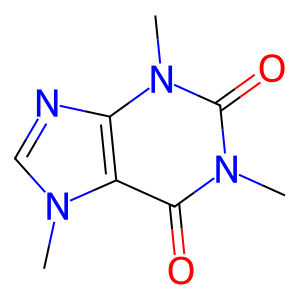
\includegraphics[width =  \textwidth ]{Bachelor-Thesis-Template/images/molecules/molecule1.png}
\end{minipage}%
\begin{minipage}{0.33\textwidth}
  \centering
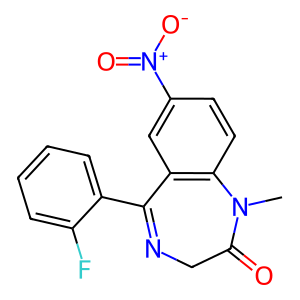
\includegraphics[width =  \textwidth ]{Bachelor-Thesis-Template/images/molecules/molecule2.png}
\end{minipage}%
\begin{minipage}{0.33\textwidth}
  \centering
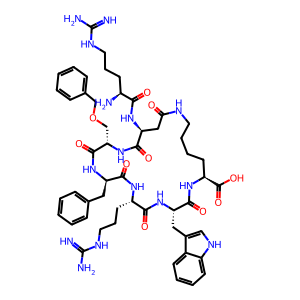
\includegraphics[width =  \textwidth ]{Bachelor-Thesis-Template/images/molecules/molecule3.png}
\end{minipage}%
\newline
\begin{minipage}{0.33\textwidth}
  \centering
(a)
\end{minipage}%
\begin{minipage}{0.33\textwidth}
\centering
 (b)
\end{minipage}%
\begin{minipage}{0.33\textwidth}
\centering
  (c)
\end{minipage}%
\caption{\small Графовые представления молекул.}
    \label{fig:molecules}
\end{figure}


\subsection{Исследование существующих решений}

В рамках исследования существующих методов предсказывания молекулярных свойств и получения эмбеддингов молекул были рассмотрены различные подходы, включая mol2vec \cite{mol2vec}, ChemBERTa \cite{ChemBERTa-2}, SMILES-BERT \cite{SMILESBERT} и другие. Эти методы основаны на принципах обработки естественного языка и используются для преобразования молекулярных структур в векторные представления, которые могут служить входными данными для алгоритмов машинного обучения.
\begin{itemize}
    \item Mol2vec \cite{mol2vec} — это метод, аналогичный Word2Vec в NLP, который использует необученный подход для получения векторных представлений молекулярных подструктур. Он преобразует молекулы в “предложения” и обучает модель на этих данных, что позволяет создавать векторы для новых молекул. Однако, он может столкнуться с ограничениями при работе с более сложными молекулярными структурами.

    \item ChemBERTa \cite{ChemBERTa-2} — это модель, которая использует трансформеры для предсказания свойств молекул. Она была одной из первых попыток систематически оценить трансформеры на задачах предсказания молекулярных свойств. ChemBERTa показала хорошие результаты при предварительном обучении на больших наборах данных и предоставила конкурентоспособную производительность на MoleculeNet \cite{moleculenet}, а также полезные визуализации на основе внимания. Однако, как и другие модели, основанные на трансформерах, она может требовать значительных вычислительных ресурсов.

    \item SMILES-BERT \cite{SMILESBERT} — это подход, который применяет модели BERT к данным SMILES для дизайна лекарств, химического моделирования и предсказания свойств. Этот подход использует предварительно обученные модели на различных наборах данных, таких как ZINC \cite{zinc} и PubChem \cite{pubchem}, и предоставляет веса модели для использования через библиотеку HuggingFace. Однако, использование SMILES как входных данных может привести к потере структурной информации, так как одна и та же молекула может быть представлена различными SMILES-строками.
\end{itemize}
Однако, несмотря на их потенциал, эти методы сталкиваются с определёнными ограничениями, особенно при использовании SMILES как входных данных. SMILES содержит только структурную информацию о молекуле, а также, как было упомянуто выше, одна и та же молекула может быть представлена различными SMILES-строками, что может затруднить обучение моделей и снизить точность предсказаний.

Важно отметить, что выбор метода зависит от конкретной задачи и доступных ресурсов. Например, если вам доступны большие вычислительные ресурсы, ChemBERTa может быть хорошим выбором. Если же вам нужно быстро получить векторные представления молекул, Mol2vec может быть более подходящим решением. В любом случае, все эти методы представляют собой важные инструменты в области химического моделирования и предсказания молекулярных свойств.

\subsection{Цель работы}

Целью данной работы является разработка и тестирование методов дообучения (fine-tuning) моделей трансформеров для предсказания молекулярных свойств на небольших специализированных выборках. Для достижения этой цели используются современные технологии и модели, такие как RoBERTa и MolCLR.

RoBERTa (Robustly optimized BERT approach) \cite{liu2019roberta} представляет собой улучшенную версию модели BERT, которая демонстрирует высокую эффективность в задачах обработки текста и анализа последовательностей, таких как ECFP. MolCLR (Molecular Contrastive Learning of Representations) \cite{molclr} использует метод контрастивного обучения, который позволяет моделям лучше понимать взаимосвязи между молекулярными структурами и их свойствами.

Особое внимание в данной работе уделено объединению моделей RoBERTa и MolCLR, что позволяет использовать преимущества обеих технологий. RoBERTa обеспечивает качественную обработку последовательностей, а MolCLR улучшает представление молекулярных структур через контрастивное обучение. Такое объединение позволяет значительно повысить точность предсказаний и улучшить обобщающую способность моделей.

Кроме того, в работе рассматривается возможность замены MolCLR на Graphormer, так как он лучше справляется с предсказанием свойств молекул. Graphormer сочетает преимущества графовых нейронных сетей и трансформеров, что позволяет более точно предсказывать свойства молекул, особенно для сложных молекулярных структур.

В рамках исследования проводится обучение модели Graphormer и сравнение её с MolCLR на задаче регрессии молекулярного свойства Molecular Weight. Это позволяет оценить эффективность Graphormer в сравнении с MolCLR и определить, какой подход является более оптимальным для предсказания молекулярных свойств.

Основной вклад данной работы заключается в предложении нового подхода к обучению моделей с использованием комбинированных представлений молекул, что позволяет повысить точность предсказаний на небольших выборках данных. Это исследование открывает новые возможности для эффективного применения машинного обучения в хемоинформатике и физической химии.



% Исторический контекст и значимость темы:

% История развития: Кратко опишите, как эволюционировали методы машинного обучения и почему они стали важными в хемоинформатике.
% Значимость исследования: Подчеркните, почему исследование предсказания молекулярных свойств является актуальным и какие потенциальные применения могут быть у результатов этого исследования.
% Текущие вызовы и проблемы:

% Ограниченность данных: Упомяните сложности, связанные с недостатком размеченных данных для обучения моделей, и как ваша работа стремится преодолеть эти ограничения.
% Точность предсказаний: Опишите, какие проблемы существуют с текущими моделями
\newpage
 %% Введение
    \section{Постановка задачи}
\label{sec:Chapter1} \index{Chapter1}

Работы по созданию эмбеддингов молекул можно разделить на два типа: использующие GNN и трансформеры. Оба подхода имеют ряд недостатков, заметных при использовании для решения прикладных химических задач. Например, при обучении почти никогда не используются физические свойства молекул, которые можно подавать в виде категориальных признаков. Большие модели, такие как BERT и многие типы GNN, достаточно плохо настраиваются под маленькие выборки веществ с специфическими физико-химическими свойствами. Кроме этого, на некоторых специфических молекулах трансформеры работают сильно хуже других (рис. \ref{fig:molecules} пункт б), а на молекулах со сложной структурой, с большим количеством атомов (рис. \ref{fig:molecules} пункт в) ошибаются графовые модели.
\newline
\textbf{Задачи исследования}:
\begin{enumerate}
    \setlength{\itemsep}{\smallskipamount}
    \item Параллельное обучение эмбеддингов: Используя BERT и GNN, обучить модели на молекулярных фингерпринтах и графовых представлениях с помощью известных подходов. Провалидировать полученные модели на задаче предсказывания физических свойств. Использовать дополнительную модель для управления выходами обеих моделей и применить dual-view consistency подход, который заключается в максимизации сходства между проекциями представлений молекул в проективных пространствах по различным метрикам.
    \item Файнтьюнинг моделей: Разработка алгоритма для тонкой настройки моделей под малые выборки с физическими свойствами, включая использование специализированного оптимизатора.
\end{enumerate}

\section*{Формальная постановка задачи}

\textbf{Дано:}
\begin{itemize}
  \item Множество молекул \( \mathcal{M} = \{m_1, m_2, ..., m_n\} \).
  \item Функции представления молекул в виде фингерпринтов \( f_{FP}: \mathcal{M} \rightarrow \mathbb{R}^d \) и графовых структур \( f_{G}: \mathcal{M} \rightarrow \mathbb{R}^d \).
  \item Набор физических свойств \( \mathcal{P} = \{p_1, p_2, ..., p_k\} \), соответствующих молекулам из \( \mathcal{M} \).
\end{itemize}

\textbf{Требуется:}
\begin{enumerate}
  \item Обучить модели BERT и GNN, \( \mathcal{B}: \mathbb{R}^d \rightarrow \mathbb{R}^h \) и \( \mathcal{G}: \mathbb{R}^d \rightarrow \mathbb{R}^h \), соответственно, используя известные подходы на представлениях молекул \( f_{FP}(m_i) \) и \( f_{G}(m_i) \).
  \item Провалидировать модели на задаче предсказания физических свойств \( \mathcal{P} \).
  \item Использовать дополнительную модель \( \mathcal{D} \) для управления выходами моделей BERT и GNN.
  \item Применить подход dual-view consistency, который формализуется как задача оптимизации:
  \[
  \max_{\mathcal{B}, \mathcal{G}} \sum_{i=1}^{n} \text{sim}\left( \mathcal{D}\left(\mathcal{B}\left(f_{FP}(m_i)\right)\right), \mathcal{D}\left(\mathcal{G}\left(f_{G}(m_i)\right)\right) \right),
  \]
  где \( \text{sim}(\cdot, \cdot) \) — метрика сходства, например, косинусное сходство.
\end{enumerate}




\newpage
 %% Постановка задачи
    \section{Обзор используемых инструментов}
\label{sec:Chapter2} \index{Chapter2}
\subsection{Языковая модель}
Языковые модели в машинном обучении играют ключевую роль в обработке и понимании естественного языка. \textit{Языковая модель} — это математическая модель, применяемая для расчета вероятности последовательности слов или фраз в естественном языке, обозначаемой как 
$$P(w_1, w_2, ..., w_n)$$
где \(w_1, w_2,..., w_n\) представляют собой токены, обычно слова или n-граммы. Вместо вычисления общей вероятности текста, часто используются модели для оценки условной вероятности 
$$P(w_n| w_1, w_2, ..., w_{n-1})$$
Эти методы являются взаимозаменяемыми, так как полная вероятность может быть выражена через условные вероятности следующим образом:
$$
P(w_1, w_2, ..., w_n) = P(w_1) \cdot P(w_2|w_1) \cdot P(w_3|w_1, w_2) \cdot ... \cdot P(w_n | w_1, w_2, ..., w_{n-1})
$$
Языковые модели лежат в основе множества задач в области обработки естественного языка, включая машинный перевод, автоматическое заполнение, классификацию текстов и другие.

Существуют различные виды языковых моделей, в том числе статистические, такие как скрытые марковские модели (HMM \cite{hmm}), и основанные на нейронных сетях, например, рекуррентные нейронные сети (RNN \cite{Das2023}) и трансформеры.

Статистические модели оценивают вероятность слов на основе их последовательности, что позволяет использовать их для предсказания следующего слова или классификации текста по тематике. Однако они ограничены в понимании контекста слов, что затрудняет их использование для генерации текста.

Нейросетевые языковые модели обучаются на больших объемах данных и могут более точно предсказывать вероятность токенов, что делает их более эффективными для генерации текста, анализа тональности и других задач обработки естественного языка.

В целом, языковые модели являются ключевым инструментом в анализе и обработке естественного языка, находя важное применение в областях, таких как компьютерная лингвистика, машинное обучение и искусственный интеллект. В данной работе, в качестве токенов будут использоваться числа из последовательности ECFP, которые представляют собой молекулярные отпечатки, позволяющие уникально идентифицировать молекулярные структуры.

В контексте машинного обучения, языковая модель представляет собой алгоритм, способный предсказывать следующий элемент в последовательности данных, основываясь на предыдущих элементах. Для текстовых данных, таких как предложения или отпечатки молекул, это означает возможность предсказывать следующее слово или символ. Модель обучается на большом объеме текстовых данных, анализируя контекст и улавливая зависимости между словами. 


\subsection{Модель RoBERTa}

\subsubsection{BPE токенизация} % Roberta
Токенизация - это процесс преобразования текстовых данных в числовой формат, с которым работают методы машинного обучения. Простейший пример токенизации - это разбить текст на части и закодировать каждую часть. Например, можно разбить текст на слова или символы и каждому уникальному слову или символу присвоить свой номер. Однако у этих подходов есть свои недостатки. При кодировании отдельных символов модели будут работать на уровне символов и будет очень сложно восстановить смысл текста по отдельным символам. Со словами возникает проблема в том, что слово может иметь много различных форм, и чтобы учесть все, нужен будет слишком большой словарь, что отрицательно скажется на производительности.

Эффективным решением данной проблемы является Byte Pair Encoding (BPE) \cite{sennrich-etal-2016-neural} токенизация. Принцип работы этого алгоритма следующий: сначала текст кодируется на уровне символов. Затем итеративно выполняются следующие шаги: \begin{itemize} 
\item Выбирается наиболее часто встречающаяся пара токенов
\item Эта пара объединяется в новый токен, и все вхождения этой пары в тексте заменяются на новый токен
\end{itemize}
Процесс повторяется до тех пор, пока размер словаря не достигнет заранее установленного предела. Такой токенизатор обучается на большом корпусе текстов и затем используется для токенизации данных на входе и выходе моделей в процессе их обучения и применения.


\subsubsection{Общая архитектура} % Roberta

\textbf{RoBERTa} (Robustly Optimized BERT Pretraining Approach) \cite{liu2019roberta} представляет собой модель, основанную на архитектуре BERT (Bidirectional Encoder Representations from Transformers) \cite{devlin2019bert}, разработанную в Facebook. Эта модель использует трансформеры для обработки последовательностей входных данных и генерации представлений слов в предложении, учитывая контекст.

\newline
RoBERTa сохраняет основную архитектуру BERT, которая является архитектурой трансформера с механизмом внимания. Математически описать это можно следующим образом:
\begin{equation}
\text{Attention}(Q, K, V) = \text{softmax}\left(\frac{QK^T}{\sqrt{d_k}}\right)V
\end{equation}
где \( Q, K, V \) обозначают матрицы запросов, ключей и значений соответственно, а \( d_k \) — размерность матрицы ключей.
\newline Основная идея BERT заключается в предварительном обучении глубоких двунаправленных представлений от неаннотированного текста, одновременно учитывая контекст слева и справа. Кроме этого, в отличие от оригинальной архитектуры трансформера, которая включает в себя энкодеры и декодеры, BERT использует только энкодеры, что делает его идеальным для задач понимания языка. Однако, в RoBERTa были внесены изменения в процесс предварительного обучения и ключевые гиперпараметры.

\newline
\textbf{Особенности RoBERTa:}
\begin{itemize}
\item RoBERTa не использует задачу Next Sentence Prediction при обучении, что улучшает или по крайней мере не ухудшает производительность на задачах нижнего уровня.
\item Более длительное обучение с большими размерами батчей, что позволяет модели лучше обобщать и достигатьл лучшей точности.
\item Динамическое маскирование: В отличие от BERT, где маскирование выполняется один раз во время предварительной обработки данных, RoBERTa использует динамическую маскирование, что позволяет модели изучать более устойчивые представления.
\item Обучение на большем объеме данных: RoBERTa была обучена на наборе данных объемом 160 ГБ, что в десять раз больше, чем набор данных, использованный для обучения BERT.
\end{itemize}

\newline Схожие модели: CamemBERT и XLM-RoBERTa являются примерами моделей, основанных на RoBERTa, которые, также как и в данной работе, были адаптированы для работы с различными языками.

\newline RoBERTa представляет собой значительное улучшение архитектуры BERT, обеспечивающее более эффективное предварительное обучение и лучшую производительность на широком спектре задач обработки естественного языка.

\subsubsection{Модель RobertaForMaskedLM} % Roberta

RobertaForMaskedLM \cite{roberta_huggingface} — это вариация модели RoBERTa, предназначенная специально для задачи Masked Language Modeling (MLM). Она отличается от стандартной модели RoBERTa тем, что включает в себя дополнительный слой RobertaLMHead, который используется для предсказания вероятности появления слова на месте маски.

% Отличия RobertaForMaskedLM от обычной модели RoBERTa:

% Специализированность: RobertaForMaskedLM оптимизирована для задач MLM, где необходимо предсказать слово, скрытое маской, на основе контекста.
% Структура: В модели RobertaForMaskedLM последний слой предназначен для предсказания маскированных токенов, в то время как стандартная модель RoBERTa может использоваться для различных задач NLP.
% RobertaLMHead — это последний слой в модели RobertaForMaskedLM, который отвечает за предсказание токенов. Этот слой принимает выходные данные из предыдущих слоёв трансформера и применяет линейное преобразование для получения распределения вероятностей по всему словарю.

\newline Принцип работы RobertaForMaskedLM представлен на рисунке \ref{fig:RoBERTaForMaskedLM}. RobertaLMHead получает векторы скрытых состояний от предыдущих слоёв трансформера. Скрытые состояния проходят через линейный слой, который преобразует их в векторы, размерность которых соответствует размеру словаря. Далее применяется функция softmax для получения распределения вероятностей по словарю (здесь модель предсказывает вероятность каждого слова оказаться на месте маскированного токена). 

\begin{figure}[!h]
    \centering
    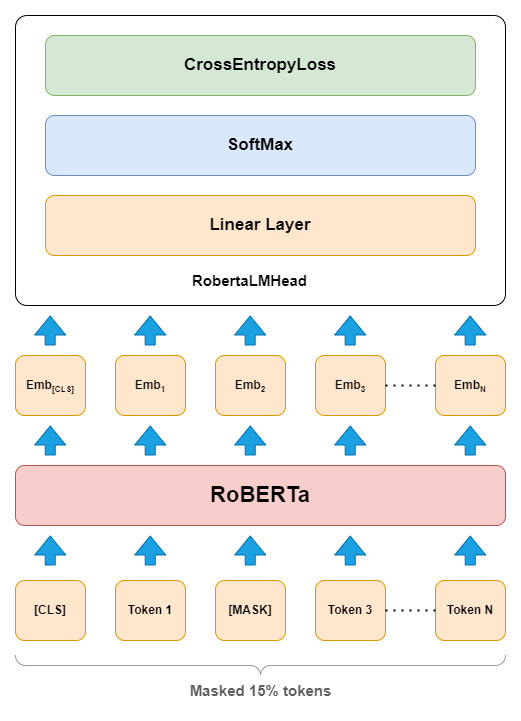
\includegraphics[width = 0.5 \textwidth ]{Bachelor-Thesis-Template/images/robertaMLM.png}
    \caption{\small Принцип работы RoBERTaForMaskedLM.}
    \label{fig:RoBERTaForMaskedLM}
\end{figure}


\newline В дополнительном слое RobertaLMHead используется функция потерь CrossEntropyLoss для вычисления ошибки между предсказанными моделью вероятностями и истинными метками. Это стандартный подход при обучении моделей MLM, таких как RoBERTa. 

Функция CrossEntropyLoss вычисляет, насколько предсказания модели отличаются от фактических меток: 
\begin{equation}
\text{CrossEntropyLoss}(y, \hat{y}) = -\sum_{i} y_{i} \log(\hat{y}_{i})
\end{equation}
где y — истинные метки, а $\hat{y}$ — предсказанные вероятности модели, а суммирование происходит по всем классам (словам в словаре). Функция потерь штрафует модель больше, если предсказанная вероятность для истинного класса низкая, и наоборот, меньше штрафует, если вероятность высокая. Это побуждает модель улучшать свои предсказания с каждой итерацией обучения.

\newline Важно отметить, что веса из слоя встраивания (embedding layer), который преобразует входные токены в векторы, используются повторно для линейного преобразования в RobertaLMHead, что позволяет уменьшить общее количество параметров модели и улучшить её обобщающую способность. Это также известно как “weight tying” в контексте языковых моделей.

\newline В контексте MLM это означает, что модель учится предсказывать вероятность каждого слова в словаре для маскированного токена, и функция потерь оценивает, насколько хорошо модель справляется с этой задачей.

\subsection{ECFP}

\subsubsection{Определение}
\textbf{Extended-Connectivity Fingerprints} - это тип молекулярных отпечатков, специально предназначенных для выявления молекулярных особенностей, связанных с молекулярной активностью. Они являются одними из самых популярных инструментов поиска сходства при разработке лекарств и эффективно используются в самых разных областях применения.

\subsubsection{Алгоритм генерации}
\begin{enumerate}
\item \textbf{Инициализация}: Каждому атому в молекуле присваивается уникальный целочисленный идентификатор, который генерируется путем хеширования комбинации свойств атома.
\item \textbf{Обновление}: На каждом этапе итерации алгоритма ECFP, идентификаторы атомов обновляются путем сбора информации от соседних атомов и применения хеш-функции для создания нового уникального идентификатора.
\item \textbf{Дедупликация}: Удаляются дублирующиеся особенности из сгенерированного списка особенностей, чтобы каждая уникальная подструктура была представлена однократно.
\newline
\newline Эти шаги повторяются для всех атомов в молекуле, позволяя сформировать массив уникальных числовых идентификаторов, которые представляют различные подструктуры молекулы. После завершения всего процесса каждый атом будет иметь идентификатор, который будет содержать субструктурную информацию со всех частей молекулы. Полученный массив чисел может быть использован для анализа молекулярных структур и моделирования структуры. 
\end{enumerate}


\subsubsection{Использование в языковой модели}
Языковые модели могут быть полезны для работы с последовательностями ECFP (Extended Connectivity Fingerprints), которые являются числовым представлением молекулярных структур. Использование языковых моделей в этом контексте может помочь в предсказании эмбеддингов молекул, что, в свою очередь, может облегчить решение различных задач, связанных с молекулярным моделированием и анализом.

Языковые модели (особенно те, что основаны на нейронных сетях, такие как BERT или Graph Neural Networks) могут изучать сложные зависимости и паттерны в данных. Они способны обрабатывать последовательности токенов и предсказывать вероятности следующих токенов и/или их векторные представления. В случае ECFP, которые кодируют информацию о химической структуре молекул, языковые модели могут использоваться для генерации представлений, которые отражают молекулярные свойства и потенциальные биологические активности.

Таким образом, подавая ECFP в качестве входных данных для языковой модели, можно обучить модель предсказывать эмбеддинги, которые могут быть использованы для различных приложений, таких как поиск похожих молекул, предсказание фармакологических свойств или оптимизация молекулярных структур для улучшения желаемых характеристик.
Важно отметить, что успех такого подхода зависит от качества и количества обучающих данных, а также от способности модели обрабатывать специфику молекулярных фингерпринтов. Это может потребовать тонкой настройки и адаптации существующих языковых моделей под конкретные задачи в области химии и молекулярной биологии.


\subsubsection{Применение к BPE токенизатору}
В рамках исследования был предложен подход к применению алгоритма Byte Pair Encoding (BPE) \cite{sennrich-etal-2016-neural} для токенизации отпечатков ECFP, представленных в виде массива чисел. Достаточно представить имеющиеся отпечатки как строку, где словами будут являться числа из массива молекулы.

\textbf{Более формально}:
Зафиксируем молекулу. Пусть \( E = \{e_1, e_2, \ldots, e_n\} \) будет её массивом ECFP, где каждый элемент \( e_i \) представляет собой целочисленное значение, полученное в результате хеширования молекулярных подструктур. Этот массив преобразуется в строку \( S \), где каждое число \( e_i \) представлено как отдельное слово (слова разделены пробелом):
$$ S = "e_1\ e_2\ \ldots\ e_n" $$

Далее, к строке \( S \) применяется алгоритм BPE, который итеративно заменяет наиболее часто встречающиеся пары чисел на новые токены, уменьшая тем самым размер словаря и обеспечивая компактное представление входных данных для модели.

Экспериментальные результаты показали, что предложенный метод токенизации ECFP с использованием BPE позволяет трансформерам эффективно обрабатывать молекулярные данные, сохраняя при этом значимую информацию о структуре и свойствах молекул.

\subsubsection{Сравнение с SMILES}
В отличие от SMILES, которые представляют линейную последовательность символов для описания молекул, ECFP генерируют векторы, которые кодируют более сложную информацию о молекуле, включая её топологическое расположение и химические свойства. Это делает ECFP особенно полезными для задач, где требуется улавливать сложные молекулярные взаимодействия и свойства, таких как предсказание биологической активности или свойств связывания.

\subsection{Графовая модель}
Графовые нейронные сети (GNN) - это тип искусственных нейронных сетей, предназначенный для работы с данными, структурированными в виде графов. Графы — это математические конструкции, которые используются для представления объектов и их связей, где узлы — объекты, а ребра — связи между ними.

В отличие от обычных нейронных сетей, которые созданы для ввода в виде сетки, GNN работают непосредственно с графами. Они способны изучать представления на уровне узлов и графов, которые полезны для широкого круга задач. Например, GNN можно использовать для задач классификации узлов, целью которых является присвоение метки каждому узлу в графе на основе его характеристик и характеристик его соседей. GNN также можно использовать для задач классификации графов, целью которых является прогнозирование свойств всего графа на основе его структуры и особенностей.

В контексте молекулярных структур, графовые нейронные сети могут быть особенно полезны. Молекулы можно представить в виде графов, где атомы являются узлами, а химические связи - ребрами. GNN могут быть использованы для изучения этих молекулярных графов, предсказания их свойств, и даже для генерации новых потенциальных молекул для лекарственного дизайна. Это делает GNN мощным инструментом в области компьютерной химии и биоинформатики.



\subsection{Модель GCN}
Graph Convolutional Network (GCN) \cite{kipf2017semisupervised} - это класс графовых нейронных сетей, который использует операцию свертки в контексте графовых структур данных. Основное отличие слоя GCN от линейного слоя заключается в том, что GCN учитывает структуру графа и связи между узлами при обновлении своих весов.

В традиционных нейронных сетях линейные слои применяют линейное преобразование к входным данным. Это преобразование преобразует входные характеристики $x$ в скрытые векторы $h$ с использованием матрицы весов $\mathbf{W}$. Если на время не учитывать смещения, это можно выразить как: 
$$h = \mathbf{W}x$$

С данными графа добавляется дополнительный слой сложности через связи между узлами. Эти связи важны, потому что, как правило, в сетях предполагается, что похожие узлы скорее будут связаны друг с другом, чем непохожие, явление, известное как гомофилия сети.

Мы можем обогатить наше представление узла, объединив его характеристики с характеристиками его соседей. Эта операция называется сверткой или агрегацией по соседству. Давайте обозначим окрестность узла i, включая сам узел, как $N_{i}$
$$h_{i} = \sum_{j \in N_{i}}\mathbf{W}x_{j}$$

Наши сверточные нейронные сети (CNN) отличаются тем, что у нас есть уникальная матрица весов $\mathbf{W}$, которая используется всеми узлами. Однако мы сталкиваемся с проблемой: количество соседей у узлов не фиксировано, в отличие от пикселей.

Чтобы значения для всех узлов были сопоставимы и находились в одном диапазоне, мы можем нормализовать результат, учитывая степень узлов, где под степенью понимается количество связей узла.
$$h_{i} = \frac{1}{deg(i)} \sum_{j \in N_{i}}\mathbf{W}x_{j}$$

Введенный Кипфом и др. (2016), у слоя графовой свертки есть еще одно улучшение.
Авторы заметили, что признаки от узлов с большим количеством соседей распространяются гораздо легче, чем от более изолированных узлов. Чтобы компенсировать этот эффект, они предложили присваивать большие веса признакам от узлов с меньшим количеством соседей, тем самым балансируя влияние по всем узлам. Эта операция записывается как
\begin{equation}
h_{i} = \sum_{j \in N_{i}} \frac{1}{\sqrt{deg(i)deg(j)}} \mathbf{W}x_{j}
\end{equation}

Существуют различные модификации слоя GCN, которые вносят улучшения или изменения в базовую модель GCN для улучшения производительности или адаптации к конкретным типам задач. Например, некоторые модификации могут включать в себя различные стратегии агрегации информации из соседних узлов или использование различных типов весовых матриц.

В отношении известных моделей, использующих GCN, можно отметить, что GCN является основой для многих других архитектур графовых нейронных сетей. Например, Graph Attention Networks (GAT) \cite{veličković2018graph} и Message Passing Neural Networks (MPNN) \cite{maskey2022generalization} являются двумя известными архитектурами, которые используют GCN в качестве основы.


\subsection{Модель MolCLR}
Molecular Contrastive Learning of Representations (MolCLR) \cite{molclr} была представлена в работе Юянга Ванга и его коллег в 2022 году. Основная архитектура модели представлена на рисунке \ref{fig:MolCLR}.

MolCLR использует подход контрастного обучения для обучения представлений молекул на больших неразмеченных наборах данных (порядка 10 миллионов молекул). Этот подход значительно улучшает производительность моделей графовых нейронных сетей на различных задачах прогнозирования свойств молекул.

В основе MolCLR лежит идея, что молекулы, которые имеют схожую структуру или свойства, должны иметь близкие представления в пространстве признаков. Для достижения этого MolCLR использует Contrastive Loss: модель обучается минимизировать расстояние между позитивными парами (то есть молекулами, которые считаются схожими) и максимизировать расстояние между негативными парами (то есть молекулами, которые считаются различными).

В модели MolCLR используются слои GCN \cite{kipf2017semisupervised} или GIN (Graph Isomorphism Network \cite{kim2020understanding}) для кодирования графов молекул. Эти слои графовых нейронных сетей позволяют модели эффективно обрабатывать структурную информацию о молекулах и извлекать из нее полезные признаки.

В данном подходе предлагаются три стратегии аугментации графа молекул: маскирование атомов, удаление связей и удаление подграфов. Эти аугментации применяются к графам молекул, чтобы создать “позитивные” пары (то есть пары аугментаций из одной и той же молекулы), которые модель стремится приблизить в пространстве признаков. 

\begin{figure}[!h]
    \centering
    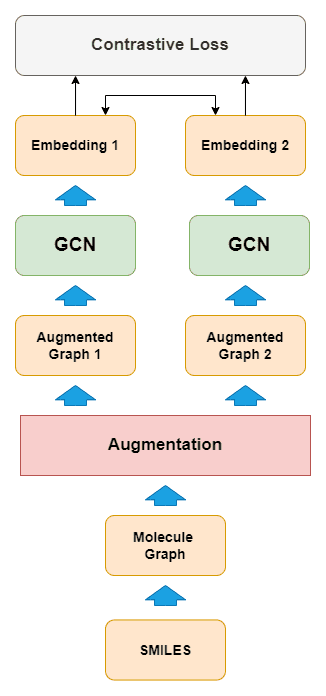
\includegraphics[width = 0.4 \textwidth ]{Bachelor-Thesis-Template/images/molclr/molclr.png}
    \caption{\small Архитектура модели MolCLR.}
    \label{fig:MolCLR}
\end{figure}

После предварительного обучения с использованием контрастного обучения, MolCLR может быть дообучена на конкретной задаче прогнозирования свойств молекул, такой как прогнозирование растворимости или токсичности.

Важно отметить, что благодаря предварительному обучению на больших неразмеченных наборах данных, MolCLR показывает хорошие результаты на различных задачах прогнозирования свойств молекул.

\subsection{Модель Graphormer}
\textbf{Graphormer} \cite{graphormer} — это модель глубокого обучения, разработанная Microsoft Research Asia и основанная на архитектуре Transformer, адаптированная для работы с графами. Основное отличие Graphormer заключается в эффективном кодировании структурной информации графа в модель, что достигается за счет использования специальных методов структурного кодирования. Она показала отличные результаты в различных задачах представления графов, особенно в рамках OGB Large-Scale Challenge.

Graphormer может быть полезен по нескольким причинам:
\begin{enumerate}
    \item Graphormer эффективно кодирует структурную информацию графа, что делает его подходящим для моделирования молекулярных структур.
    \item Данная модель показала отличные результаты на широком диапазоне задач обучения представлению графов.
    \item Graphormer может быть использован для обучения пользовательских моделей для задач моделирования молекул.
    \item Graphormer может покрывать многие популярные варианты GNN в качестве своих специальных случаев.
\end{enumerate}

Для подготовки данных к обучению Graphormer необходимо использовать специальную функцию collate, которая группирует признаки нескольких графов в батчи. Это позволяет эффективно подавать данные в модель. Предобработка включает в себя преобразование данных в формат, совместимый с Graphormer, включая создание объектов DGLGraph и использование стандартного PyTorch Dataloader для подачи данных в модель.

Обучение Graphormer включает в себя стандартные этапы, такие как маскирование части входных данных и предсказание вероятностей для замаскированных элементов. Важно отметить, что модель может неэффективно работать с очень большими графами (более 100 вершин), так как это может привести к переполнению памяти. В таких случаях рекомендуется уменьшить размер батча или использовать более мощные вычислительные ресурсы.



\subsection{Графовое представление молекул}

\begin{enumerate}
    \item  Узлы представляют собой молекулярные атомы. Каждый узел имеет свой уникальный идентификатор (например, атомный номер) и может содержать дополнительные атрибуты (например, химические свойства атома).
    \item Рёбра соединяют узлы и представляют химические связи между атомами. В графовых представлениях молекул обычно используются два типа рёбер:
    \begin{itemize}
        \item \texttt{edge\_index}: Это список пар узлов, которые соединены рёбрами. Например, если у нас есть ребро между атомами 1 и 2, то (1, 2) будет присутствовать в \texttt{edge\_index}. Таким образом, размер этого поля $2*|E|$, где $|E|$ – количество рёбер в графе.
        \item \texttt{edge\_attr}: Это матрица признаков рёбер, таких как тип связи (одинарная, двойная, тройная) или расстояние между атомами.
    \end{itemize}
    \item Атрибуты узлов (\texttt{node\_attr}): Это матрица, состоящая их дополнительных характеристик каждого узла. Например, масса атома, заряд, гибридизация и т. д.
    \item Количество узлов (\texttt{num\_nodes}): Это общее количество атомов в молекуле.
\end{enumerate}
В графовых моделях, таких как MolCLR и Graphormer, на вход графы подаются в формате, который содержит данные поля, поэтому они играют важную роль в обучении подобных моделей.

\subsection{Библиотека RDKit}
\textbf{RDKit} \cite{RDKit} – это библиотека для хемоинформатики и машинного обучения, написанная на C++ и Python. RDKit предоставляет множество функций для работы с молекулами, включая чтение, отображение, запись и многие другие операции.
Есть возможность создавать молекулы из SMILES-кодов, файлов формата MOL и блоков данных MOL, а также поддерживается отображение молекул в виде графических изображений.
 
Пример получения обьекта молекулы из SMILES: 
$$\texttt{rdkit.Chem.MolFromSmiles('Cc1ccccc1')}$$

\subsection{Датасет ChemBL}
\textbf{ChEMBL} \cite{ChemBL} – это база данных биоактивных молекул с лекарственными свойствами. Она объединяет химические, биоактивные и геномные данные для поддержки перевода геномной информации в эффективные новые лекарства.

На основе данных из данного датасета можно получить молекулярные фингерпринты или SMILES и обучить модель машинного обучения для регрессии молекулярных свойств, используя различные алгоритмы, такие как графовые нейронные сети (GNN), регрессию или другие методы. Таккже можно использовать датасет ChEMBL для тестирования полученных моделей, так как он предоставляет информацию о биоактивных молекулах и их свойствах.

\subsection{Оптимизатор AdamW}}
\textbf{AdamW} \cite{adamw} — один из самых эффективных алгоритмов оптимизации для обучения нейронных сетей. Это модификация оптимизационного алгоритма Adam (adaptive moment estimation), который сочетает в себе идеи RMSProp и оптимизатора импульса. Adam использует адаптивную оценку моментов первого и второго порядка.
\begin{itemize}
    \item Основная идея AdamW заключается в добавлении метода декремента весов (weight decay) к Adam.
    \item Декремент весов помогает бороться с переобучением, регуляризуя модель.
    \item AdamW более устойчив к большим значениям весов и улучшает обобщающую способность модели.
\end{itemize}

\subsection{Функции потерь}
\subsubsection{L1-Loss}
Для L1-потерь обычно используется MAE (Mean Absolute Error):
\begin{equation}
L1 = \sum_{i=1}^{N} |y_i - \hat{y}_i|
\end{equation}
где $N$ - количество элементов во входе $y$, $y_i$ - фактическое значение для i-го примера, а $\hat{y}_i$ - предсказанное значение для i-го примера.

\subsubsection{MSE-Loss}
Функция потерь Mean Squared Error (MSE) измеряет среднеквадратичную ошибку (квадрат нормы L2) между каждым элементом входа x и целевым значением y. Она описывается следующим образом:
\begin{equation}
\ell(y, \hat{y}) = \frac{1}{N} \sum_{n=1}^{N} (y_n - \hat{y}_i)^2 
\end{equation}
где $N$ - количество элементов во входе $y$, $y_i$ - фактическое значение для i-го примера, а $\hat{y}_i$ - предсказанное значение для i-го примера.

\subsubsection{CosineSimilarityLoss}
\textbf{Cosine Similarity Loss} используется для измерения сходства между двумя векторами на основе косинусного сходства. Это часто применяется для оценки степени схожести между векторами. Значение косинусного сходства находится в диапазоне от -1 до 1, где 0 указывает на ортогональность, а значения, близкие к 1 по модулю, указывают на большее сходство.
Формула косинусного расстояния:
\begin{equation}
sim(x_1, x_2) = \frac{x_1 * x_2}{max(\lVert x_1 \rVert * \lVert x_2 \rVert, \epsilon)}
\end{equation}

\subsubsection{NTXentLoss}
\textbf{NT-XentLoss} (Normalized Temperature-scaled Cross Entropy Loss) — это функция потерь, используемая в глубоком обучении. Она измеряет косинусное сходство между двумя векторами и использует параметр температуры для балансировки положительных и отрицательных пар. Пусть $sim(u, v)$ обозначает косинусное сходство между векторами u и v. Тогда функция потерь для положительной пары примеров (i, j) выглядит следующим образом:

\begin{equation}
l_{i, j} = -\log\left(\frac{e^{sim(u_i, v_j) / \tau}}{\sum_{k=1}^{N} e^{sim(u_i, v_k) / \tau}}\right)
\end{equation}

где $sim(u_i, v_j)$ - косинусное сходство между векторами $u_i$ и $v_j$, $N$ - общее количество примеров, $\tau$ (температура) - параметр, который регулирует вклад положительных и отрицательных пар.

Эта функция потерь позволяет обучать эмбеддинги так, чтобы они были близки для положительных пар и далеки для отрицательных пар, что полезно для задач, связаных с поиском сходства между векторами, например, в задачах ранжирования или рекомендации.


\newpage
 %% Обзор существующих решений
    \section{Исследование и построение решения задачи}
\label{sec:Chapter3} \index{Chapter3}




\subsection{Декомпозиция задачи}
Для решения поставленной задачи необходимо разбить её на ряд подзадач, каждая из которых должна быть достаточно простой для непосредственного решения. Процесс декомпозиции включает в себя следующие шаги:

\begin{enumerate}
\item \textbf{Сбор требований и анализ проблемы:}
\begin{itemize}
    \item Определение целей исследования и задач, которые необходимо решить.
    \item Исследование существующих решений и определение их ограничений.
\end{itemize}

\item \textbf{Исследование и выбор подходов:}
\begin{itemize}
    \item Анализ различных методов и технологий, применимых для решения задачи.
    \item Оценка плюсов и минусов различных моделей и подходов на основе научных публикаций и предыдуших исследований.
    \item Выбор оптимального подхода для каждой из подзадач.
\end{itemize}

\item \textbf{Проектирование архитектуры системы:}
\begin{itemize}
    \item Разработка общей архитектуры решения, включающей интеграцию всех компонентов.
    \item Определение взаимодействий между различными частями системы (например, как данные будут передаваться между моделями RoBERTa и GNN).
\end{itemize}

\item \textbf{Подготовка данных:}
\begin{itemize}
    \item Сбор исходных данных.
    \item Очистка данных от выбросов и слишком больших молекул.
    \item Нормализация данныхю
    \item Преобразование данных в необходимые форматы (ECFP и графовое представление).
    \item Предобработка данных для Graphormer (добавление необходимых полей, обьединение графов в батчи).
\end{itemize}

\item \textbf{Разработка и настройка моделей:}
\begin{itemize}
    \item Разработка и настройка токенайзера для модели RoBERTa.
    \item Определение и настройка архитектур для модели GNN.
    \item Настройка модели Graphormer.
    \item Подбор гиперпараметров для моделей.
    \item Выбор наиболее подходящей модели для задачи.
    \item Разработка baseline-модели, которая объединяет в себе два подхода.
\end{itemize}

\item \textbf{Обучение и тестирование моделей:}
\begin{itemize}
    \item Обучение модели RoBERTa с использованием Masked Language Modeling.
    \item Обучение моделей GNN: MolCLR и Graphormer.
    \item Тестирование обученных моделей на валидационном наборе данных.
\end{itemize}

\item \textbf{Интеграция и согласование эмбеддингов:}
\begin{itemize}
    \item Проекция эмбеддингов из различных моделей в общее пространство.
    \item Оптимизация сходства эмбеддингов с использованием метрик, таких как косинусное расстояние.
\end{itemize}

\item \textbf{Анализ и интерпретация результатов:}
\begin{itemize}
    \item Проведение экспериментов для оценки качества полученных эмбеддингов.
    \item Интерпретация результатов и формулирование выводов.
\end{itemize}

\end{enumerate}

\newpage
 %% Исследование и построение решения задачи
    \section{Описание практической части}
\label{sec:Chapter4} \index{Chapter4}

В это разделе описываются все проведенные эксперименты, а также их результаты. Важно отметить, что все вставляемые фрагменты кода используют библиотеки PyTorch \cite{pytorch}, RDKit \cite{RDKit} и HuggingFace \cite{huggingface}, а также предполагают наличие определенных глобальных переменных и конфигураций, которые не указаны в коде.


\subsection{Препроцессинг данных}
Препроцессинг данных начинается с использования библиотеки RDKit \cite{RDKit} для преобразования строковых представлений молекул в формате SMILES в структурированные графовые объекты. Это позволяет перевести химическую информацию, содержащуюся в SMILES, в формат, который может быть эффективно обработан современными графовыми нейронными сетями.

\begin{enumerate}
    \item Импорт необходимых модулей из библиотеки RDKit, определение списков атомов, хиральности и типов связей (были взяты стандартные списки из RDKit).
    
    \item Создание функции \texttt{get\_graph\_columns}, которая принимает SMILES-строку и возвращает графовое представление молекулы (матрицу связей, признаки узлов, рёбер, а также количество узлов в графе).
    
    \item Применение функций RDKit для преобразования SMILES в объект молекулы, из которого затем извлекается информация об атомах и связях для создания графового представления.
    
    \item Построения матрицы признаков узлов графа (для чего используются кодирование атомных номеров, хиральностей и типов связей).
    
    \item Применение функции \texttt{get\_graph\_columns} к стоблцу датасета, содержащему SMILES.
\end{enumerate}

Этот процесс позволяет преобразовать большое количество молекул, представленных в виде SMILES, в структурированные графовые данные для предсказания молекулярных свойств с помощью GNN. 

Данный препроцессинг производится над датасетом ChemBL \cite{ChemBL}, где содержатся также необходимые отпечатки молекул, которые будут использоваться как вход для трансформера.


\subsection{Обучение RoBERTa}
Обучение модели RoBERTa для задач хемоинформатики требует специальной настройки и адаптации стандартных процедур обучения трансформеров. В этом разделе описывается процесс настройки токенайзера, методика обучения с маскированием и тестирование обученной модели, а также анализ полученных результатов.

\subsubsection{Настройка токенайзера}
Используя библиотеку HuggingFace \cite{huggingface}, был создан ByteLevelBPETokenizer. Процесс настройки включает в себя следующие этапы:

\begin{enumerate}
    \item Обучение токенайзера на полученных файлах с целью создания словаря токенов и правил их слияния. Параметры обучения включают размер словаря, минимальную частоту токенов и специальные токены ($<s>, <pad>, </s>, <unk>, <mask>$).
    
    \item Сохранение обученного токенайзера, включая файлы \texttt{vocab.json} и \texttt{merges.txt}, которые содержат информацию о словаре токенов и правилах слияния.
    
    \item Тестирование токенайзера на примере молекулярной последовательности для проверки корректности токенизации и присвоения идентификаторов токенам.
\end{enumerate}
Токенайзер позволяет уменьшить размер словаря. Это позволяет снизить размерность пространства наших значений хеш-функции (используемой в алгоритме ECFP) с $2^{32}$ до размерности пространства токенов (примерно 10000).

\subsubsection{Обучение маскированием}
Методика обучения с маскированием (Masked Language Modeling, MLM) является ключевой для обучения модели RoBERTa. Этот подход позволяет модели учиться предсказывать исходные значения замаскированных токенов, что способствует лучшему пониманию контекста и структуры молекул. В качестве основы была взята модель \texttt{RobertaForMaskedLM} из библиотеки HuggingFace \cite{huggingface}. Процесс обучения включает следующие шаги:

\begin{enumerate}
    \item Использование функции маскирования \texttt{mlm}, которая создает случайную маску для 15\% токенов в тензоре, исключая специальные токены, такие как начало (<s>), конец последовательности (<s/>) и паддинг(<pad>).
    
    \item Применение функции \texttt{tokenize\_ecfps} для токенизации и маскирования ECFP последовательностей, подготовки входных данных, масок внимания и меток для обучения.
    
    \item Создание загрузчиков данных (DataLoaders) для обучающего, валидационного и тестового наборов данных, которые обеспечивают эффективную подачу данных в модель во время обучения.
    
    \item Инициализация модели \texttt{RobertaForMaskedLM} с использованием определенной конфигурации \texttt{RobertaConfig}, где задаются параметры модели (стандартный размер словаря - 30522, максимальная длина позиционных эмбеддингов - 512 + 2, стандартный для трансформера размер скрытых слоев - 768 и количество скрытых слоев - 6). Модель обучается без загрузки весов, from scratch.

    \item Инициализация оптимизатора AdamW \cite{adamw} c шагом обучения 1e-5.
    
    \item Применение цикла обучения, включающего в себя подсчет потерь, обратное распространение ошибки, шаг оптимизации и обнуление градиентов.
    
    \item Логирование функции потерь и метрик, таких как accurracy, precision recall, F1-score, с помощью инструмента \texttt{wandb} \cite{wandb} для отслеживания прогресса обучения.
    
    \item Проведение валидации модели на валидационном наборе данных для оценки ее способности к обобщению и предсказанию.
\end{enumerate}



\subsubsection{Тестирование обученной модели и результаты}
После завершения процесса обучения результаты модели RoBERTa были протестированы на независимом (тестовом) наборе данных. Использовались следующие метрики качества из библиотеки sklearn \cite{sklearn} (метки были сагрегированы как взвешенное среднее):

\begin{itemize}
    \item \textbf{\texttt{accuracy\_score}}: $0.86$ (отражает долю правильно классифицированных примеров)
    
    \item \textbf{\texttt{precision\_score}}: $0.89$ (показывает долю релевантных экземпляров среди всех экземпляров, выбранных моделью)
    
    \item \textbf{\texttt{recall\_score}}: $0.86$ (отражает способность модели обнаруживать все релевантные случаи в данных)
    
    \item \textbf{\texttt{f1\_score}}: $0.87$ (представляет собой сбалансированную меру precision и recall)
\end{itemize}

Графики точности для обучения (a), валидации (b) и тестирования (c) представлены на Рисунке \ref{fig:roberta_accuracy}. Эти графики иллюстрируют динамику изменения точности модели на различных этапах её оценки и позволяют визуально оценить уровень обобщающей способности модели и её стабильность в различных условиях.


\begin{figure}[h]
    \begin{minipage}{0.33\textwidth}
        \centering
        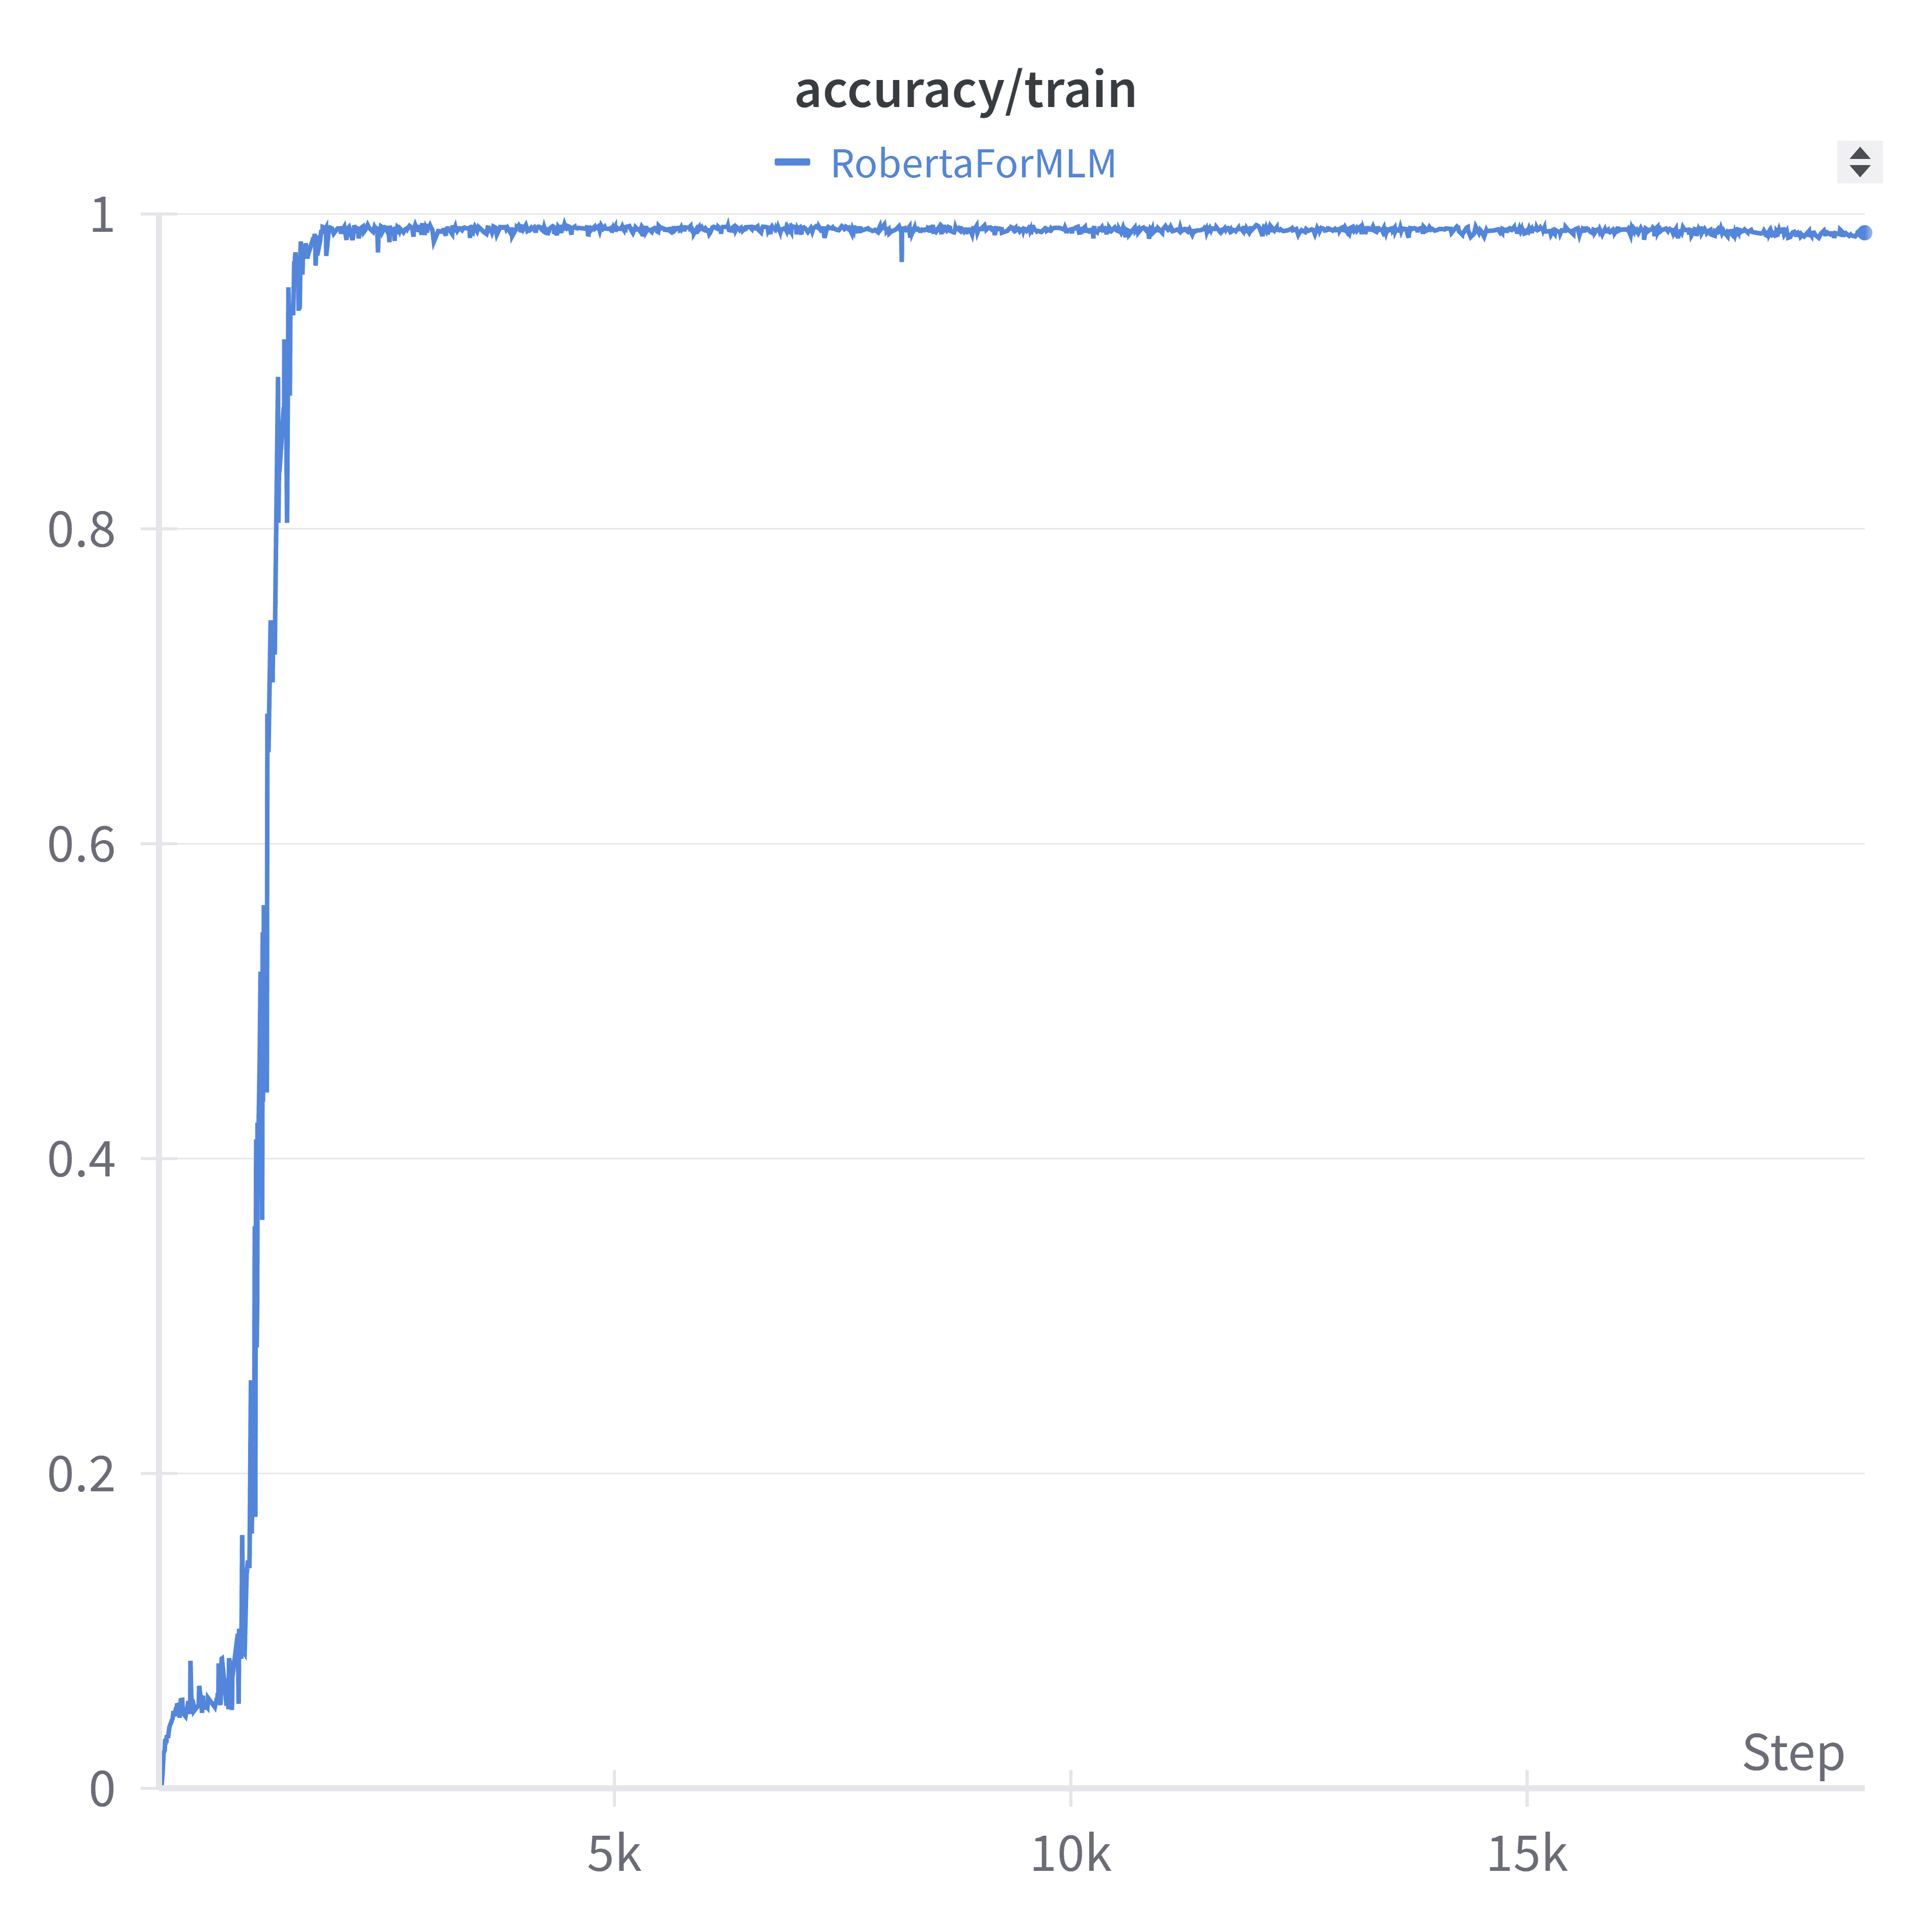
\includegraphics[width =  \textwidth ]{Bachelor-Thesis-Template/images/roberta/train/accuracy_train.png}
    \end{minipage}%
    \begin{minipage}{0.33\textwidth}
        \centering
        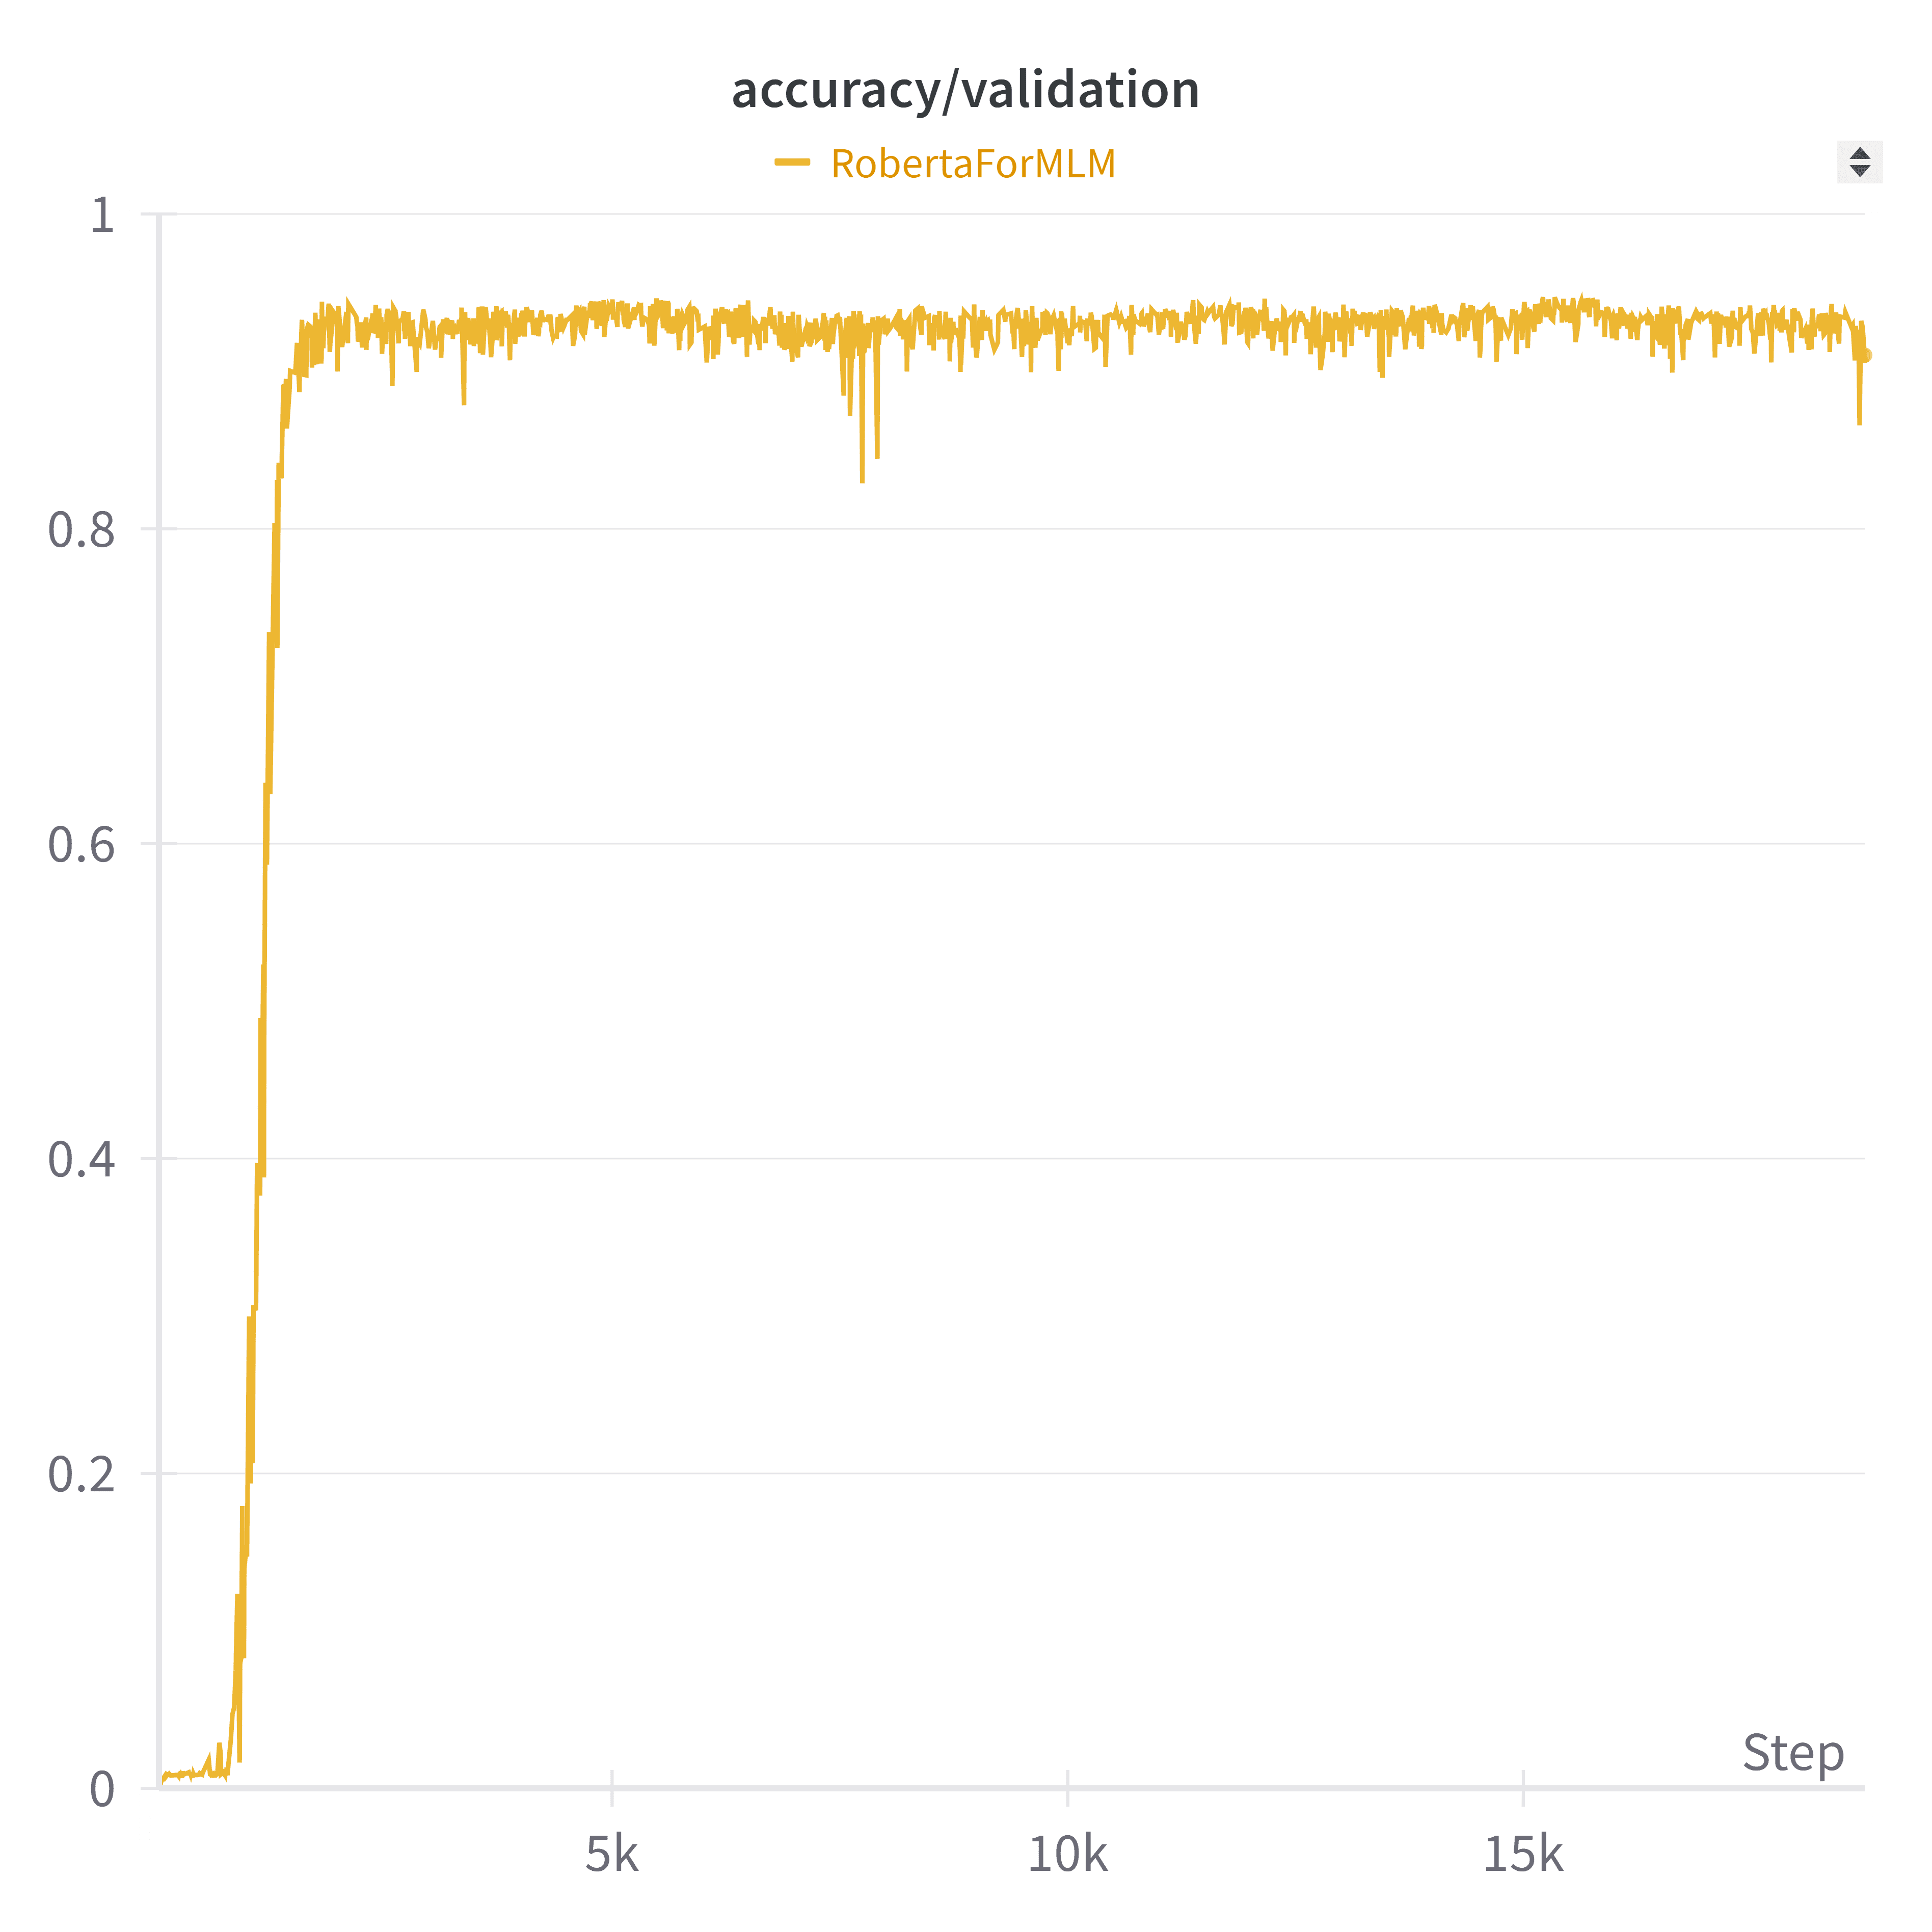
\includegraphics[width =  \textwidth ]{Bachelor-Thesis-Template/images/roberta/validation/accuracy_validation.png}
    \end{minipage}%
    \begin{minipage}{0.33\textwidth}
        \centering
        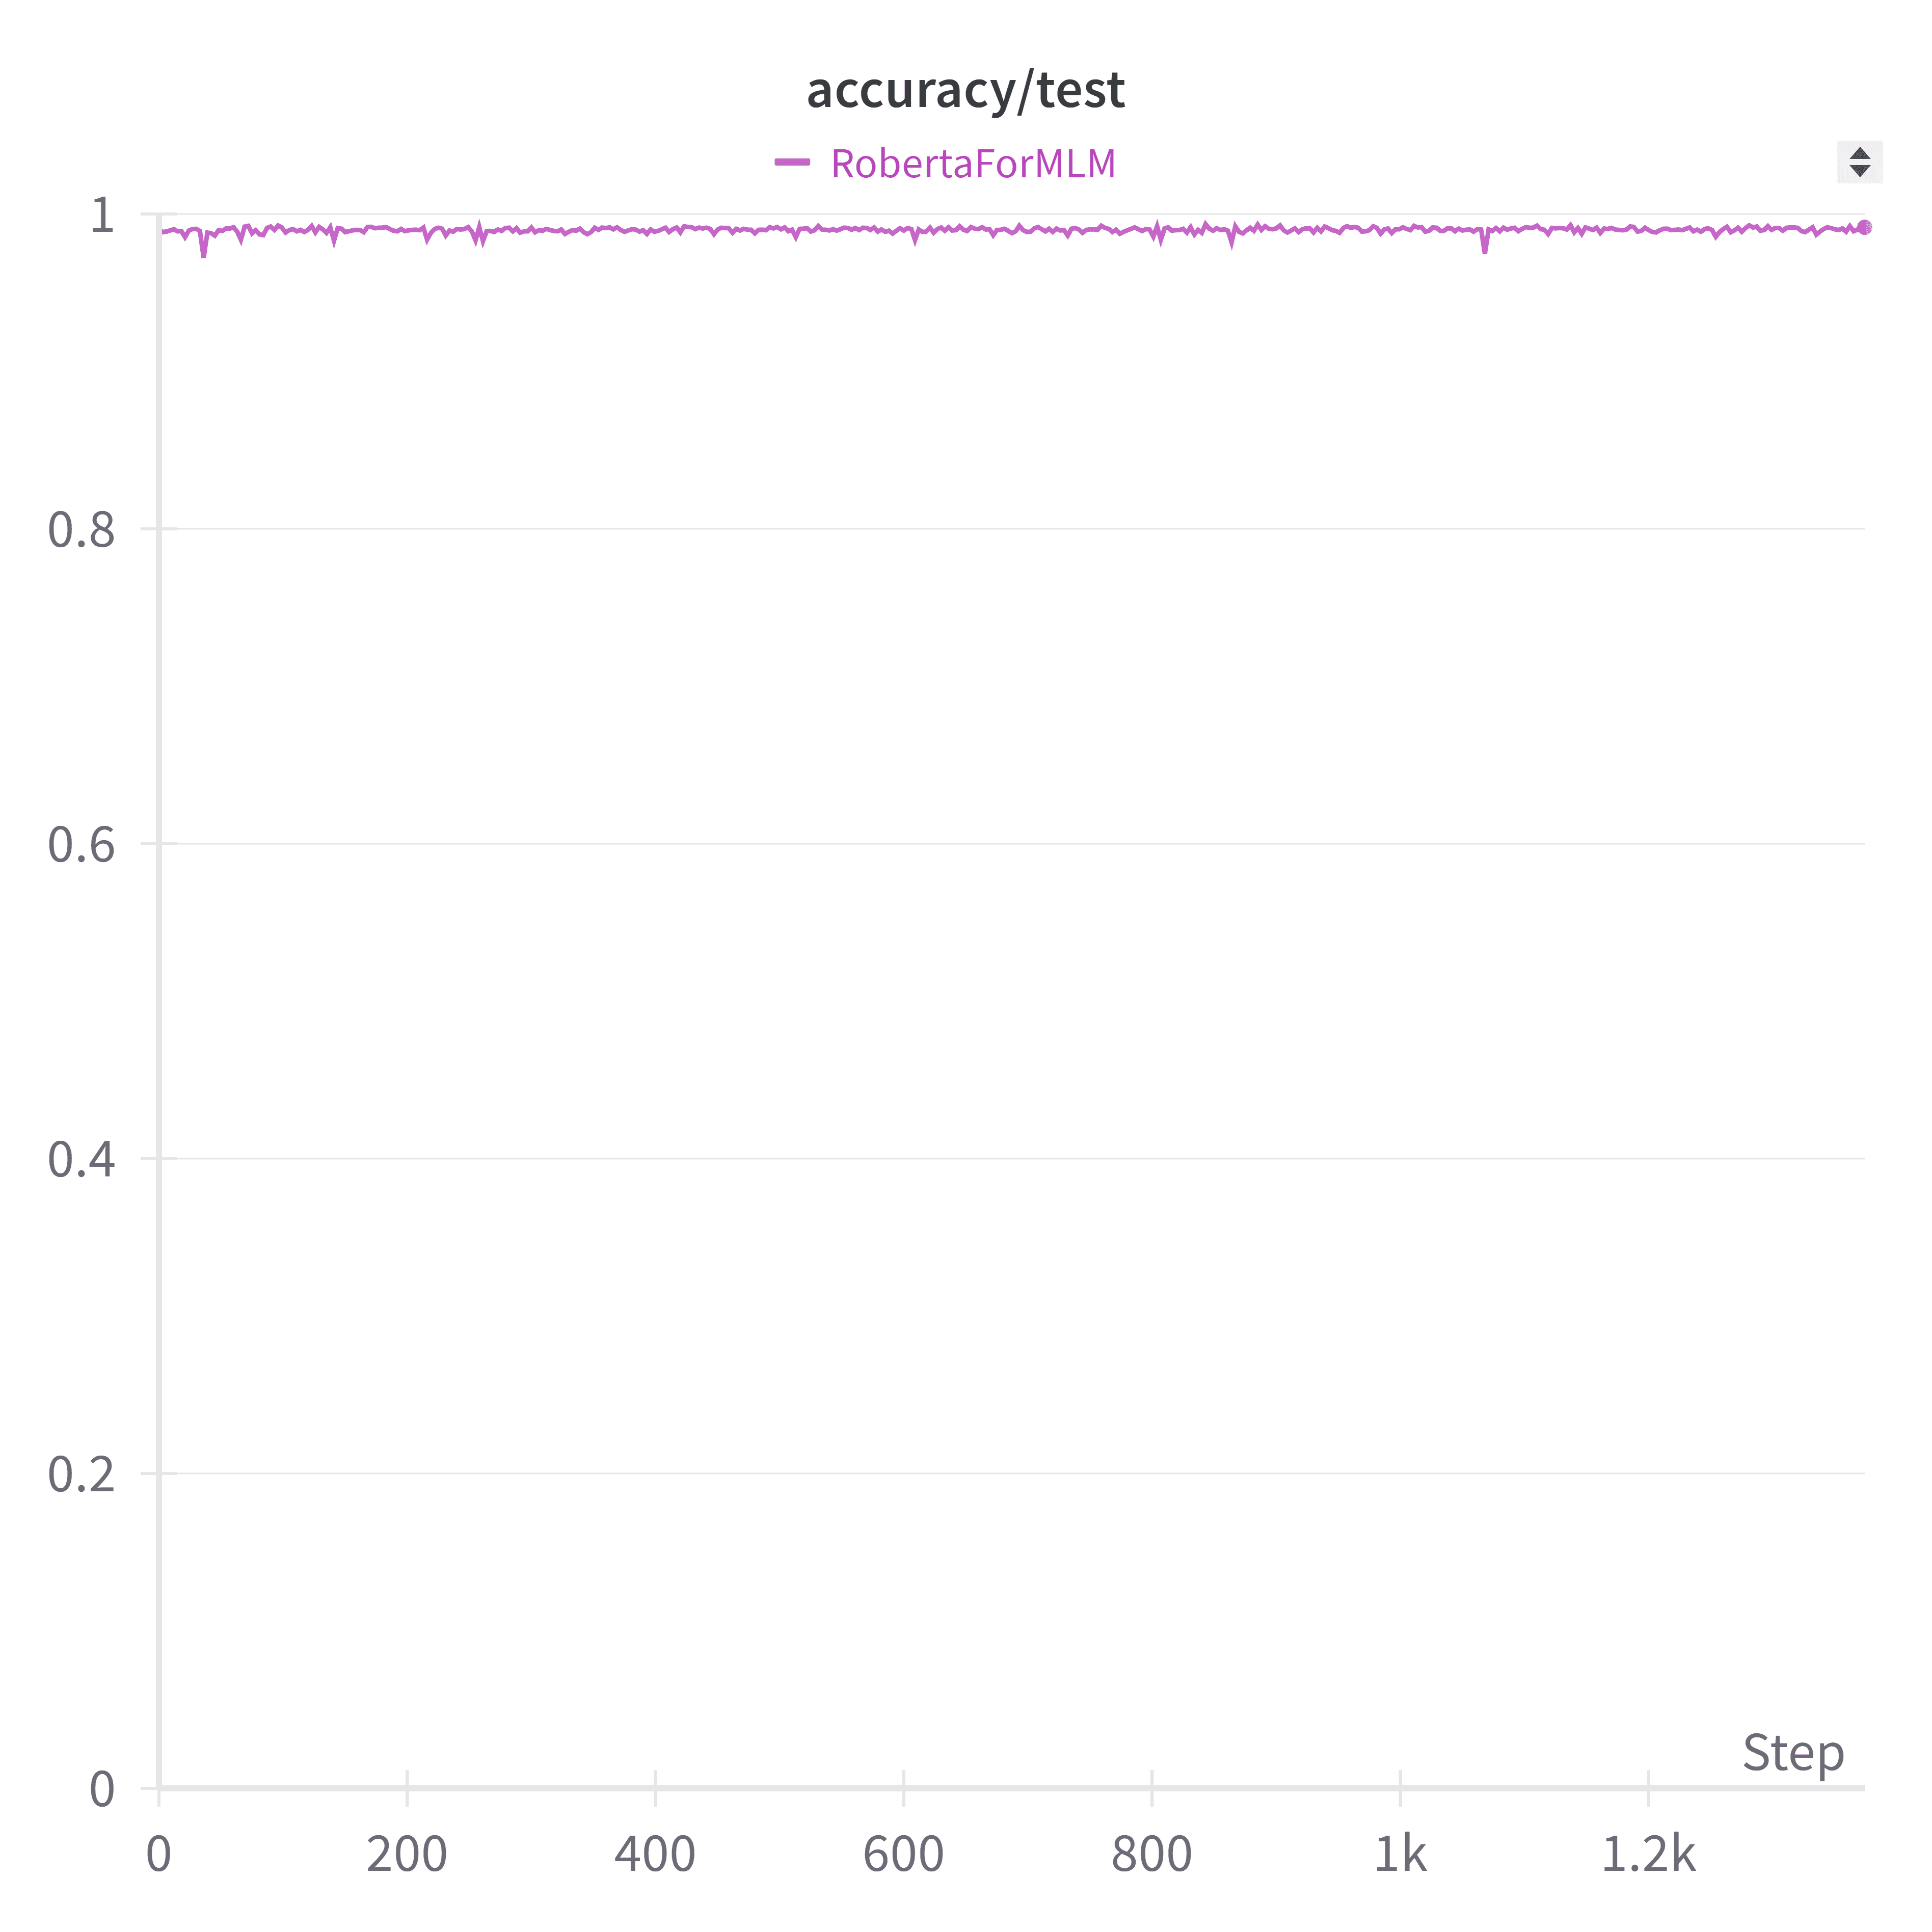
\includegraphics[width =  \textwidth ]{Bachelor-Thesis-Template/images/roberta/test/accuracy_test.png}
    \end{minipage}%

    \newline
    \begin{minipage}{0.33\textwidth}
      \centering
    \textbf{(a)}
    \end{minipage}%
    \begin{minipage}{0.33\textwidth}
    \centering
    \textbf{(b)}
    \end{minipage}%
    \begin{minipage}{0.33\textwidth}
    \centering
    \textbf{(c)}
    \end{minipage}%
    
    \caption{\small Графики метрики accuracy: (a) train, (b) validation, (c) test}
    \label{fig:roberta_accuracy}
\end{figure}

Результаты тестирования подтверждают высокую производительность модели RoBERTa в задаче предсказания молекулярных свойств, что делает её перпективным инструментом для дальнейших исследований в области хемоинформатики.

\subsection{Обучение MolCLR}
Процесс обучения включает следующие шаги:
\begin{enumerate}
\item В начале исследования был создан экземпляр \texttt{MoleculeDataset} на основе датасета ChemBL \cite{ChemBL}. Далее были определены индексы для обучающего, валидационного и тестового наборов данных. Для каждого из этих наборов данных был создан \texttt{DataLoader} из библиотеки \texttt{torch\_geometric} \cite{torch_geometric}, который использовался для итерации по данным в процессе обучения и валидации.

\item В качестве основы для обучения была выбрана самописная модель \texttt{MolecularGraph}. Эта модель включает в себя графовую модель (в зависимости от конфигурации это может быть \texttt{GINet} или \texttt{GCN}), а также линейный слой для предсказания. GNN была инициализирована с предварительно обученными весами.

\item В ходе обучения вычислялась функция потерь между предсказанными и истинными метками и выполнялось обратное распространение ошибки. В качестве метрики была выбрана L1-норма. Результатом одной эпохи было усреднение loss-функции по всей эпохе.

\newpage
\textbf{Код цикла обучения:}
\begin{lstlisting}
model = MolecularGraph().to(device)
loss_func = torch.nn.L1Loss()
def train_loop():
    train_tqdm = tqdm(train_dataloader, unit="batch")
    train_tqdm.set_description(f'Epoch {epoch_counter}')
    loss_sum = 0
    
    model.train()
    for (batch, labels_batch) in train_tqdm:
        optimizer.zero_grad()

        graph_batch = batch.to(device)
        labels_batch = labels_batch.to(device)

        predicted_labels = model(graph_batch)

        loss = loss_func(predicted_labels, labels_batch)
        loss.backward()

        loss_sum += loss.item()

        optimizer.step()
        train_tqdm.set_postfix(loss=loss.item())
    return loss_sum / len(train_dataloader)
\end{lstlisting}
\item В цикле валидации \texttt{eval\_loop()} был выполнен проход по каждому батчу в валидационном \texttt{eval\_dataloader}. Процесс был аналогичен циклу обучения, однако в этом случае веса модели не обновлялись. Валидация происходила каждую эпоху.

\item После каждой эпохи проводилось сравнение фукнции потерь на обучающем и валидационном наборах данных. Это позволило отслеживать процесс обучения и валидации модели в динамике.
\end{enumerate}


Данное обучение было проведено на 4 физических свойствах молекул: Polar Surface Area, AlogP, Bioactivities и Molecular Weight. В ходе эксперимента были получены следующие результаты. На рисунке \ref{fig:molclr_loss} представлены графики функции потерь в процессе обучения (a) и валидации (b) для этих четырех свойств.

На тестовой выборке были получены следующие значения функции потерь:

\begin{itemize}
\item Molecular Weight: 99.521
\item Polar Surface Area: 20.127
\item AlogP: 1.019
\item Bioactivities: 5.74
\end{itemize}

В данном датасете свойство Molecular Weight лежит в пределах [77.06; 1060.97] со средним 388.6, свойство Polar Surface Area лежит в пределах [0.0; 392.73] со средним 78.5. свойство AlogP лежит в пределах [-5.61; 11.97] со средним 3.33, свойство Bioactivities лежит в пределах [1.0; 3247.0] со средним 12.1. Эти данные показывают, что диапазоны и средние значения для каждого из четырех свойств существенно различаются. Поэтому, чтобы сравнить производительность модели на разных свойствах, необходимо рассмотреть относительные значения функции потерь:
\begin{itemize}
\item Molecular Weight: $99.521 / 388.6 = 0.26$
\item Polar Surface Area: $20.127 / 78.5 = 0.26$
\item AlogP: $1.019 / 3.33 = 0.31$
\item Bioactivities: $5.74 / 12.1 = 0.47$
\end{itemize}

Эти результаты указывают на то, что модель наиболее точно предсказывает свойства Molecular Weight и Polar Surface Area, в то время как для свойства Bioactivities значение функции потерь значительно выше, что может указывать на необходимость дальнейшей оптимизации модели для этого свойства.

\begin{figure}[h]
    \begin{minipage}{0.5\textwidth}
        \centering
        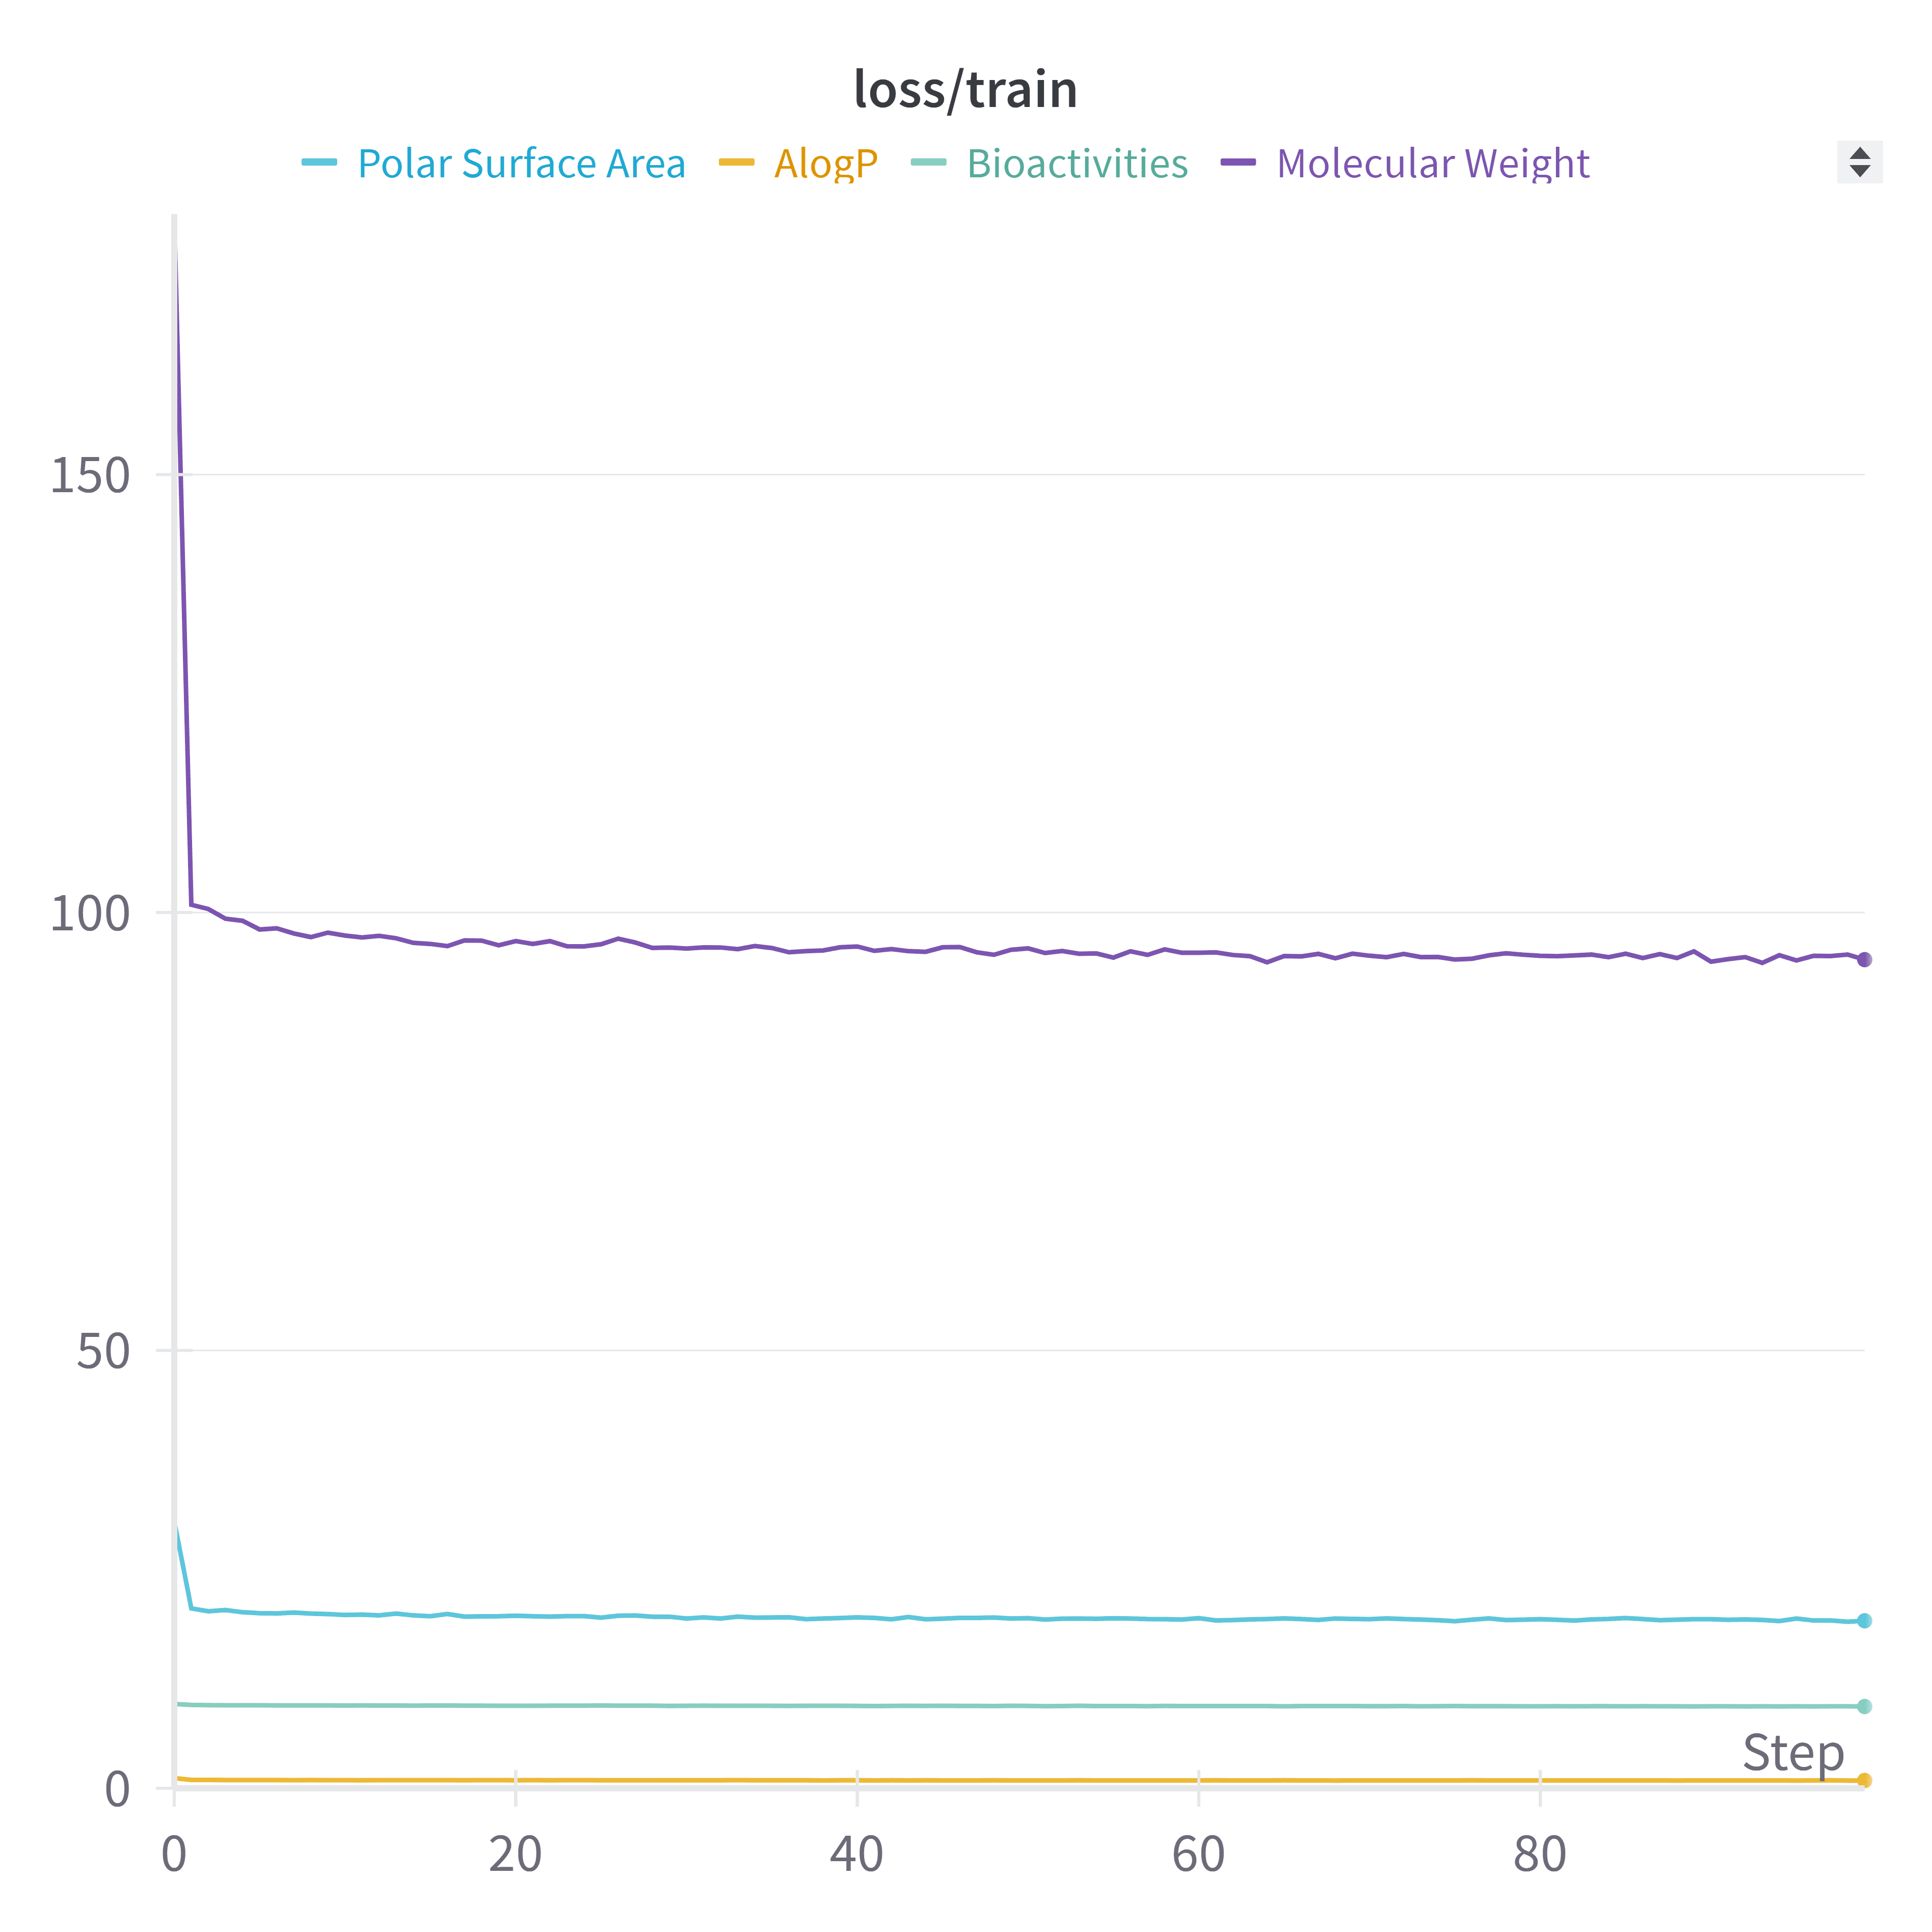
\includegraphics[width =  \textwidth ]{Bachelor-Thesis-Template/images/molclr/MolCLR loss_train.png}
    \end{minipage}%
    \begin{minipage}{0.5\textwidth}
        \centering
        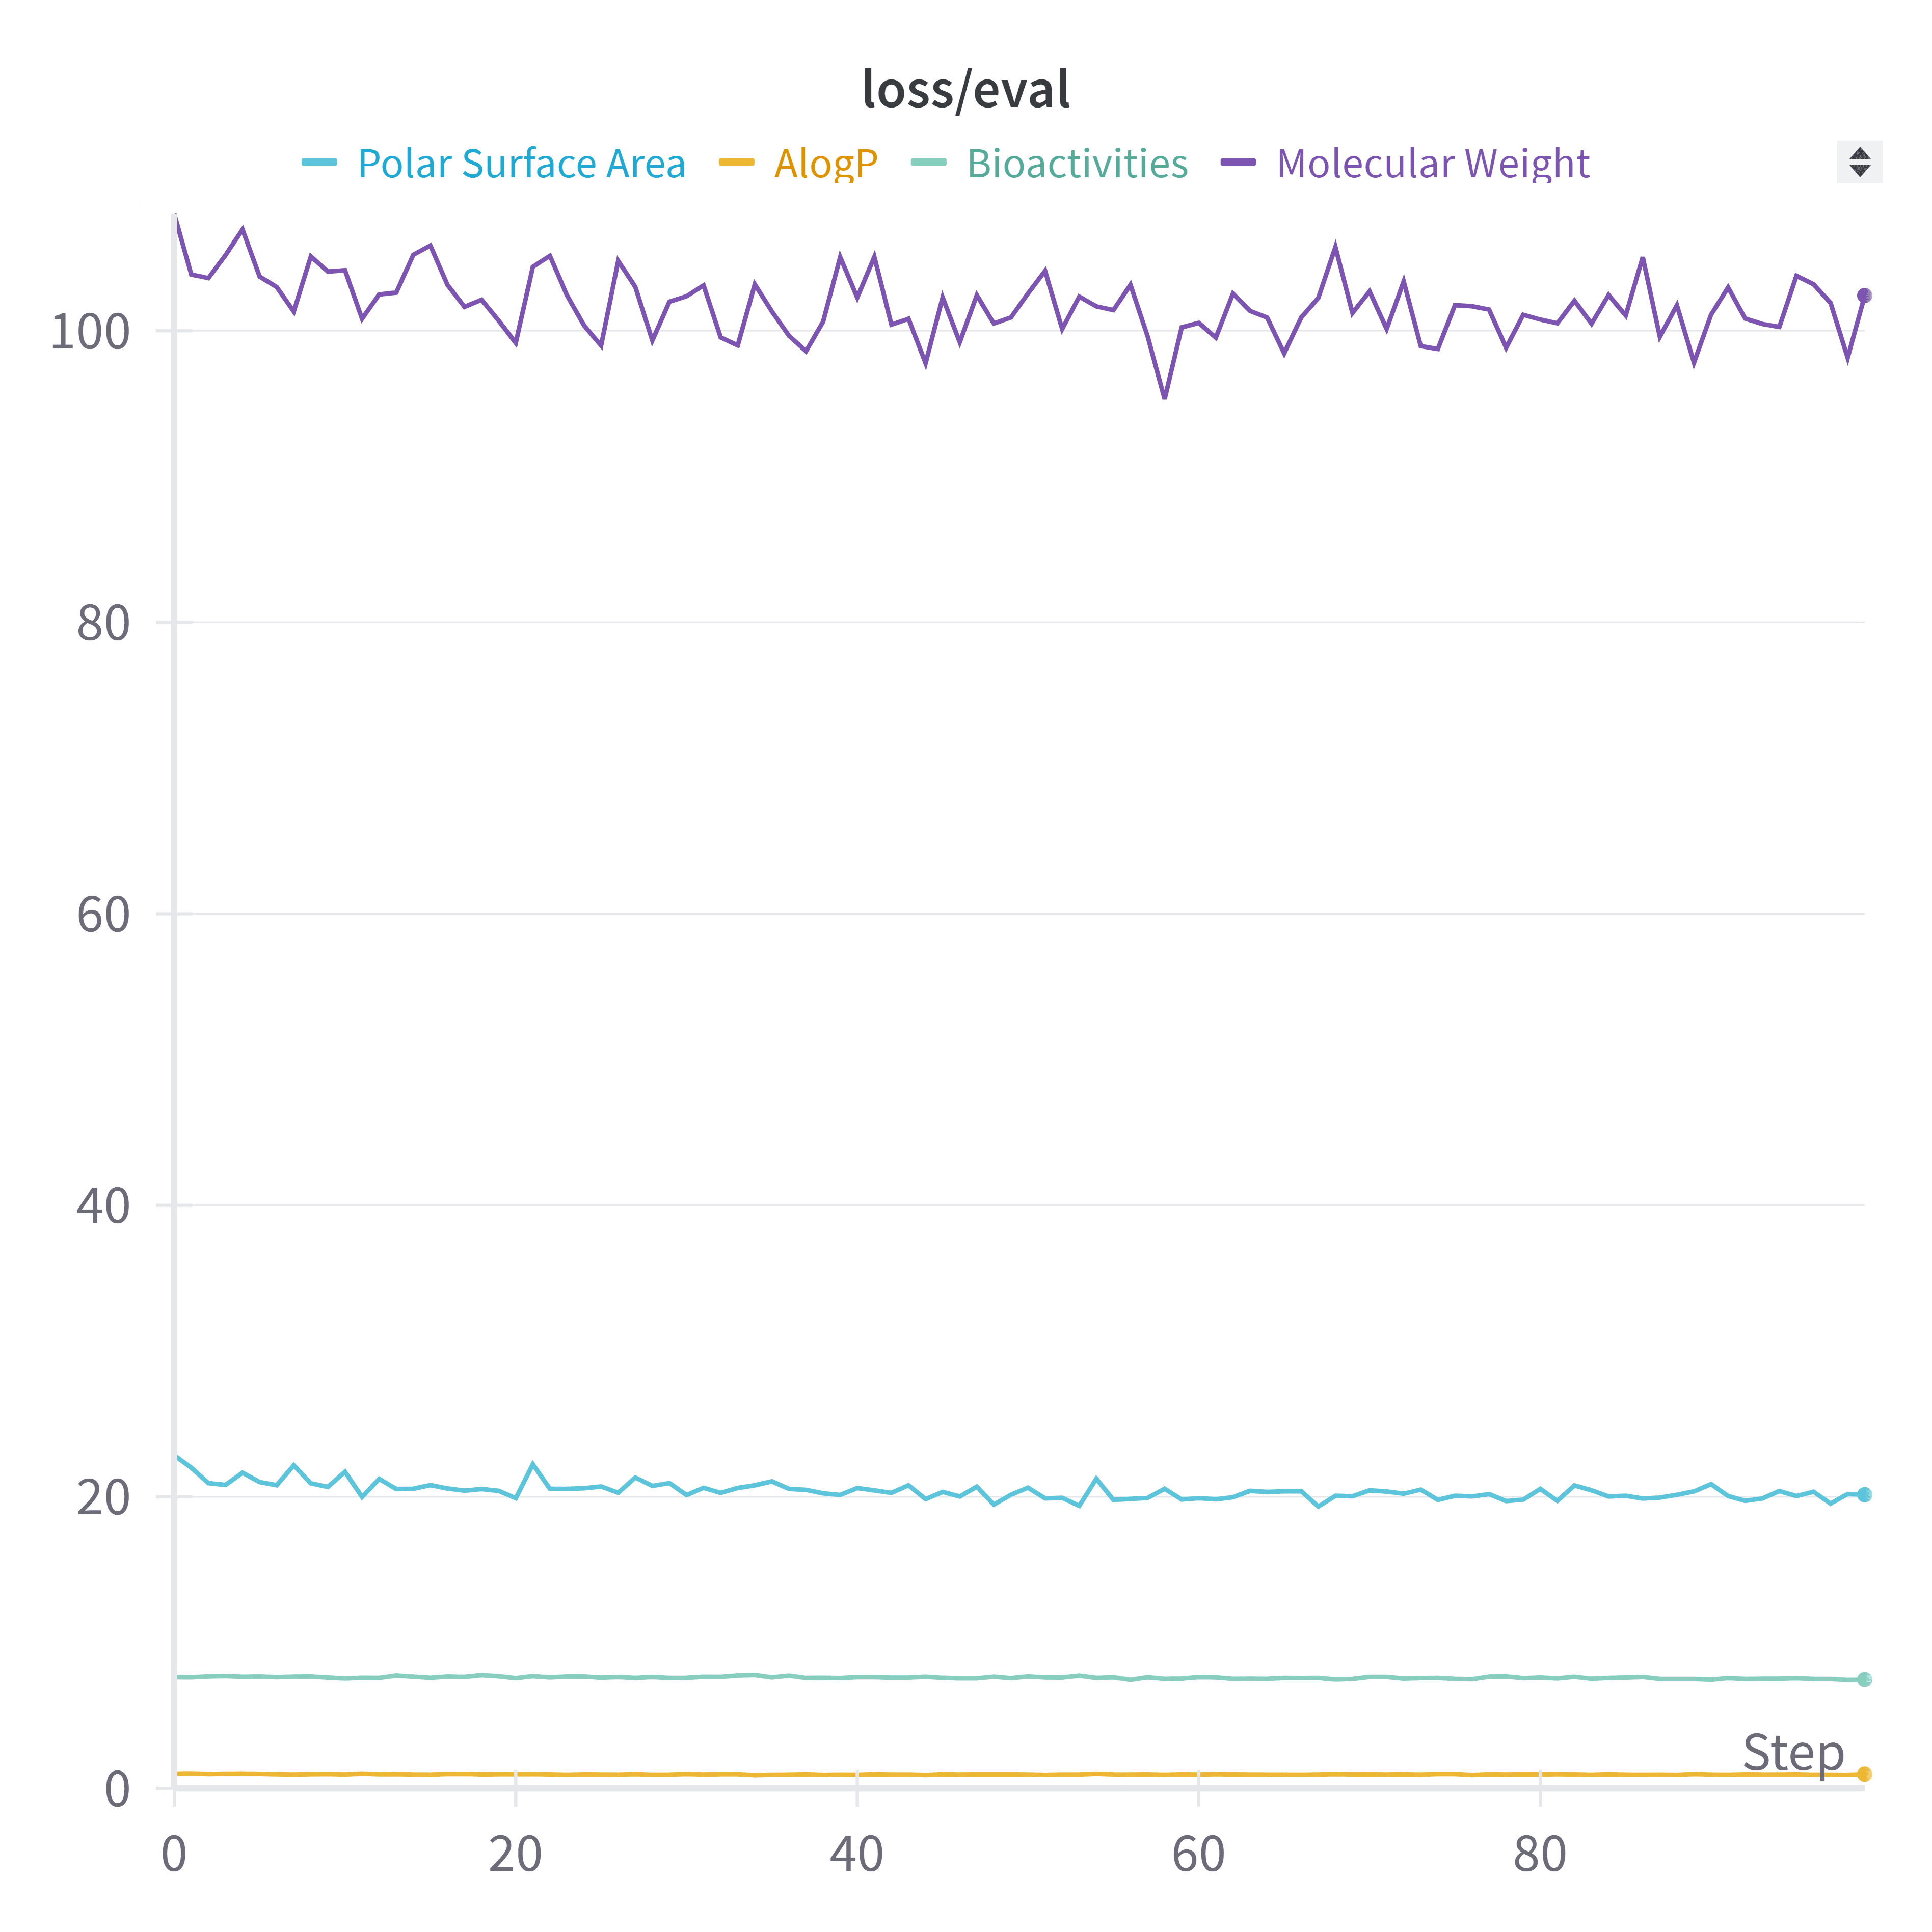
\includegraphics[width =  \textwidth ]{Bachelor-Thesis-Template/images/molclr/MolCLR loss_eval.png}
    \end{minipage}%

    \newline
    \begin{minipage}{0.5\textwidth}
      \centering
    \textbf{(a)}
    \end{minipage}%
    \begin{minipage}{0.5\textwidth}
    \centering
    \textbf{(b)}
    \end{minipage}%
    
    \caption{\small Графики функции потерь L1-loss: (a) train, (b) validation}
    \label{fig:molclr_loss}
\end{figure}
% Molecular Weight mean is 388.62499576450654
% Molecular Weight max is 1060.97
% Molecular Weight min is 77.06
% Bioactivities mean is 12.074121135112241
% Bioactivities max is 3247.0
% Bioactivities min is 1.0
% AlogP mean is 3.337519059720458
% AlogP max is 11.97
% AlogP min is -5.61
% Polar Surface Area mean is 78.52042037272342
% Polar Surface Area max is 392.73
% Polar Surface Area min is 0.0

\subsection{Обучение Graphormer}
Обучение Graphormer включает в себя использование специализированных слоёв внимания, которые позволяют модели учитывать глобальные структурные особенности графа. Этап обучения направлен на минимизацию функции потерь и оптимизацию параметров модели для достижения наилучшей производительности. В данном эксперименте используется функция потерь MSE (Mean Squared Error). Для оптимизации параметров применяется классический оптимизатор AdamW с коэффициентом обучения равным 5e-5. Кроме того, используется линейный планировщик скорости обучения.

\newcommand\wtt[1]{%
  \hfil\penalty0\hfilneg\texttt{#1}%
}

\begin{enumerate}
\item Сначала из части датасета ChemBL \cite{ChemBL} инстанцируется экземпляр класса \texttt{Dataset} библиотеки HuggingFace \cite{huggingface}. Далее идет разделение всего набора данных на обучающий, валидационный и тестовый наборы. Это дает 80\% данных для обучения, 10\% для валидации и 10\% для тестирования.

\item Затем применяется специальная функция \texttt{preprocess\_item} к каждому элементу в наборах данных. Это преобразует каждый элемент в формат, подходящий для модели Graphormer (добавляются еще 7 тензоров для каждой молекулы).

\item Инициализируется модель \texttt{GraphormerForGraphClassification} (использовался чек-поинт \texttt{clefourrier/graphormer-base-pcqm4mv1}). Также устанавливается параметр \texttt{num\_classes} равным 1, поскольку предсказывается одно свойство.

\item Инициализируется GraphormerDataCollator, который позволяет обьединять данные графов в батчи (в отличие от обычных GNN, где \texttt{torch\_geometric.data} обьекты графов подаются на вход по одному). Данный обраточик данных подается в инициализацию Dataloaders для каждого набора данных.

\item Инициализируется \textbf{оптимизаторы обучения:}
\begin{lstlisting}
from transformers import AdamW, get_scheduler

num_epoch = 100
num_training_steps = num_epoch * len(train_dataloader)

optimizer = AdamW(model.parameters(), lr=5e-5)
lr_scheduler = get_scheduler(
    'linear',
    optimizer = optimizer,
    num_warmup_steps = 5,
    num_training_steps = num_training_steps,
)
\end{lstlisting}


\item Далее исполняется стандартный \textbf{цикл обучения:}
\begin{lstlisting}
progress_bar_train = tqdm(range(num_training_steps))

model.train()
train_epoch_loss = 0
for batch in train_dataloader:
    input_batch = { k: v.to(device) for k, v in batch.items() }
    
    outputs = model(**input_batch)
    
    loss = outputs["loss"]
    loss.backward()
    train_epoch_loss += loss.item()
    
    optimizer.step()
    lr_scheduler.step()
    optimizer.zero_grad()
    progress_bar_train.update(1)
\end{lstlisting}

\item В цикле валидации итерация проходт по каждому батчу в \texttt{eval\_dataloader}. Процесс похож на цикл обучения, но здесь не обновляются веса модели.

\item После каждой эпохи сравниваются функции потерь на обучающем и валидационном наборах данных. Эти данные сохраняются с помощью  библиотеки wandb \cite{wandb}. С помощью одноименного веб-сервиса можно будет отследить, как модель обучалась и валидировалась в процессе обучения.
\end{enumerate}

Результаты работы данного алгоритма показаны на рисунке \ref{fig:graphormer_vs_molclr_loss}. На рисунке (a) изображен график обучения Graphormer с помощью регресии молекулярного свойсва Molecular Weight. Также здесь представлен график обучения модели MolCLR для сравнения результатов. Рядом, на рисунке (b), показаны результаты валидации этих двух моделей. Исходя из этих данных, понятно, что трансформер Graphormer имеет потенциал предсказывания молекулярных свойств выше, чем модель MolCLR, основанная на классической модели свертки графов. Поэтому исследуемый Graphormer может быть использован как альтернатива или дополнение к модели MolCLR.


В ходе исследования была предпринята попытка нормализации данных с использованием MinMaxScaler из библиотеки sklearn \cite{sklearn}. Однако, после нормализации данные оказывались слишком близкими к нулю, что приводило к погрешностям в вычислениях и делало графики менее информативными. В связи с этим, результаты исследования показаны с использованием исходных, ненормализованных данных для обучения модели Graphormer.



\begin{figure}[h]
    \begin{minipage}{0.5\textwidth}
        \centering
        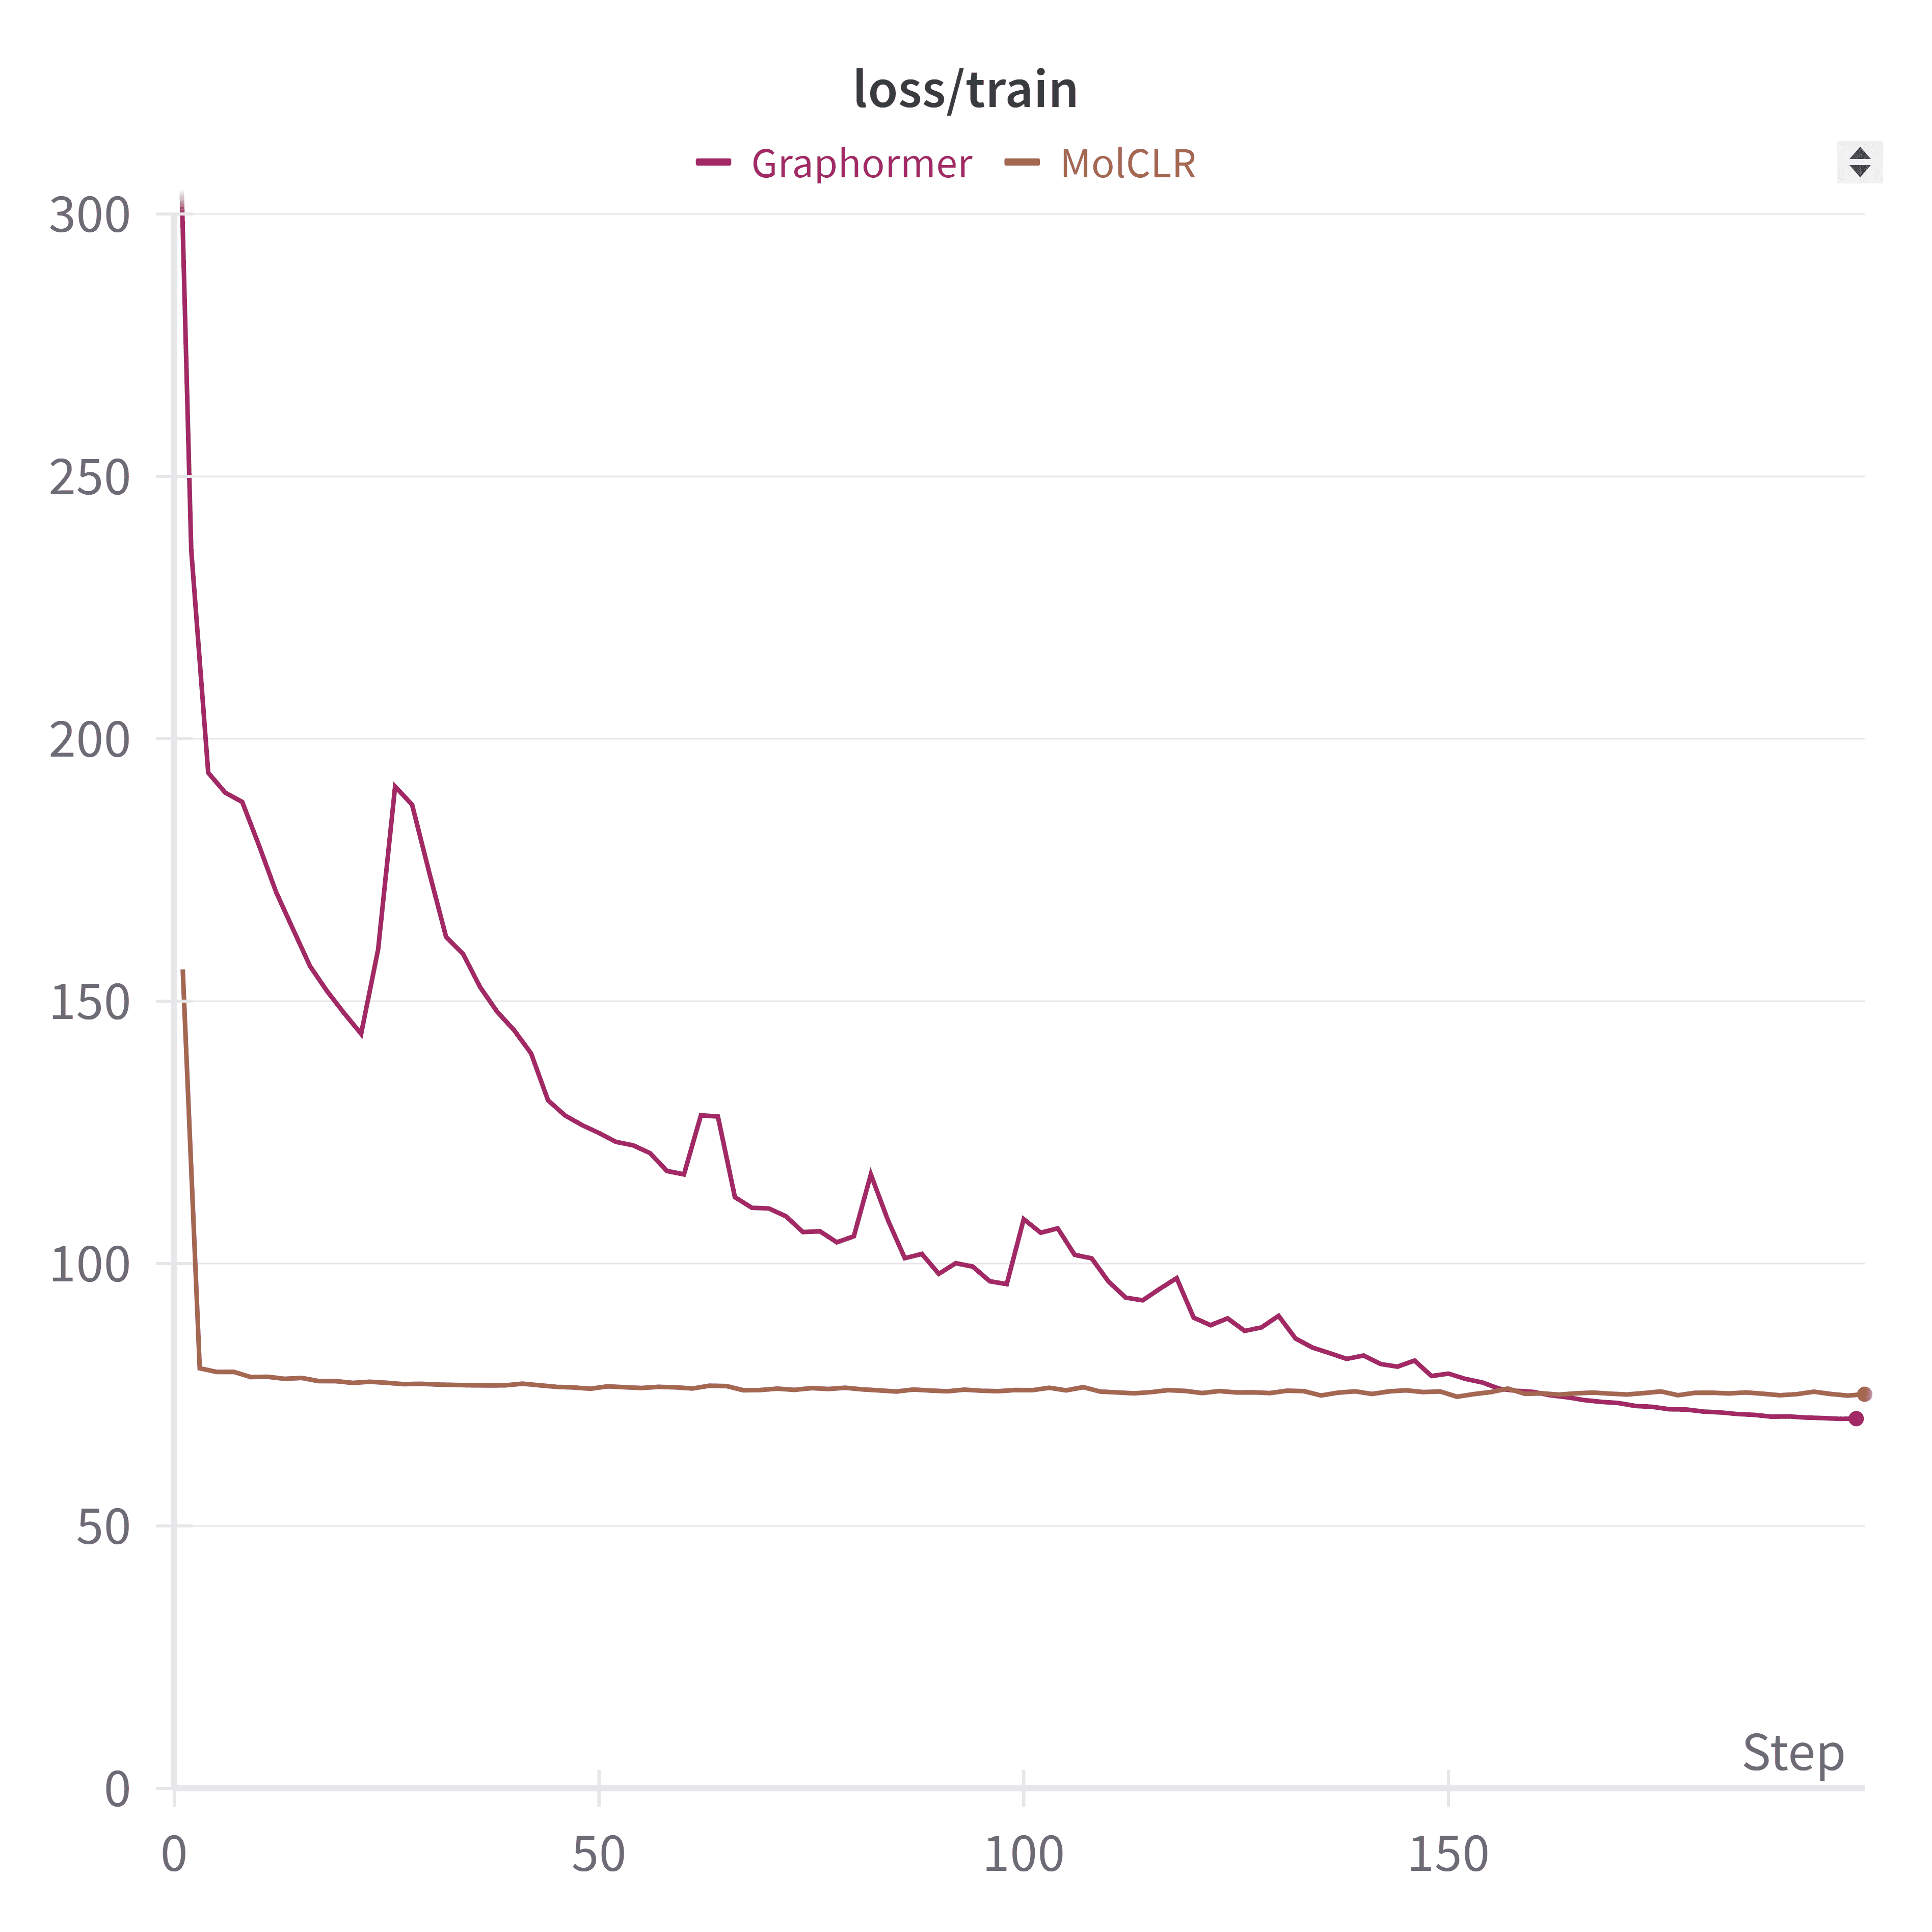
\includegraphics[width =  \textwidth ]{Bachelor-Thesis-Template/images/graphormer/train_graphormer.png}
    \end{minipage}%
    \begin{minipage}{0.5\textwidth}
        \centering
        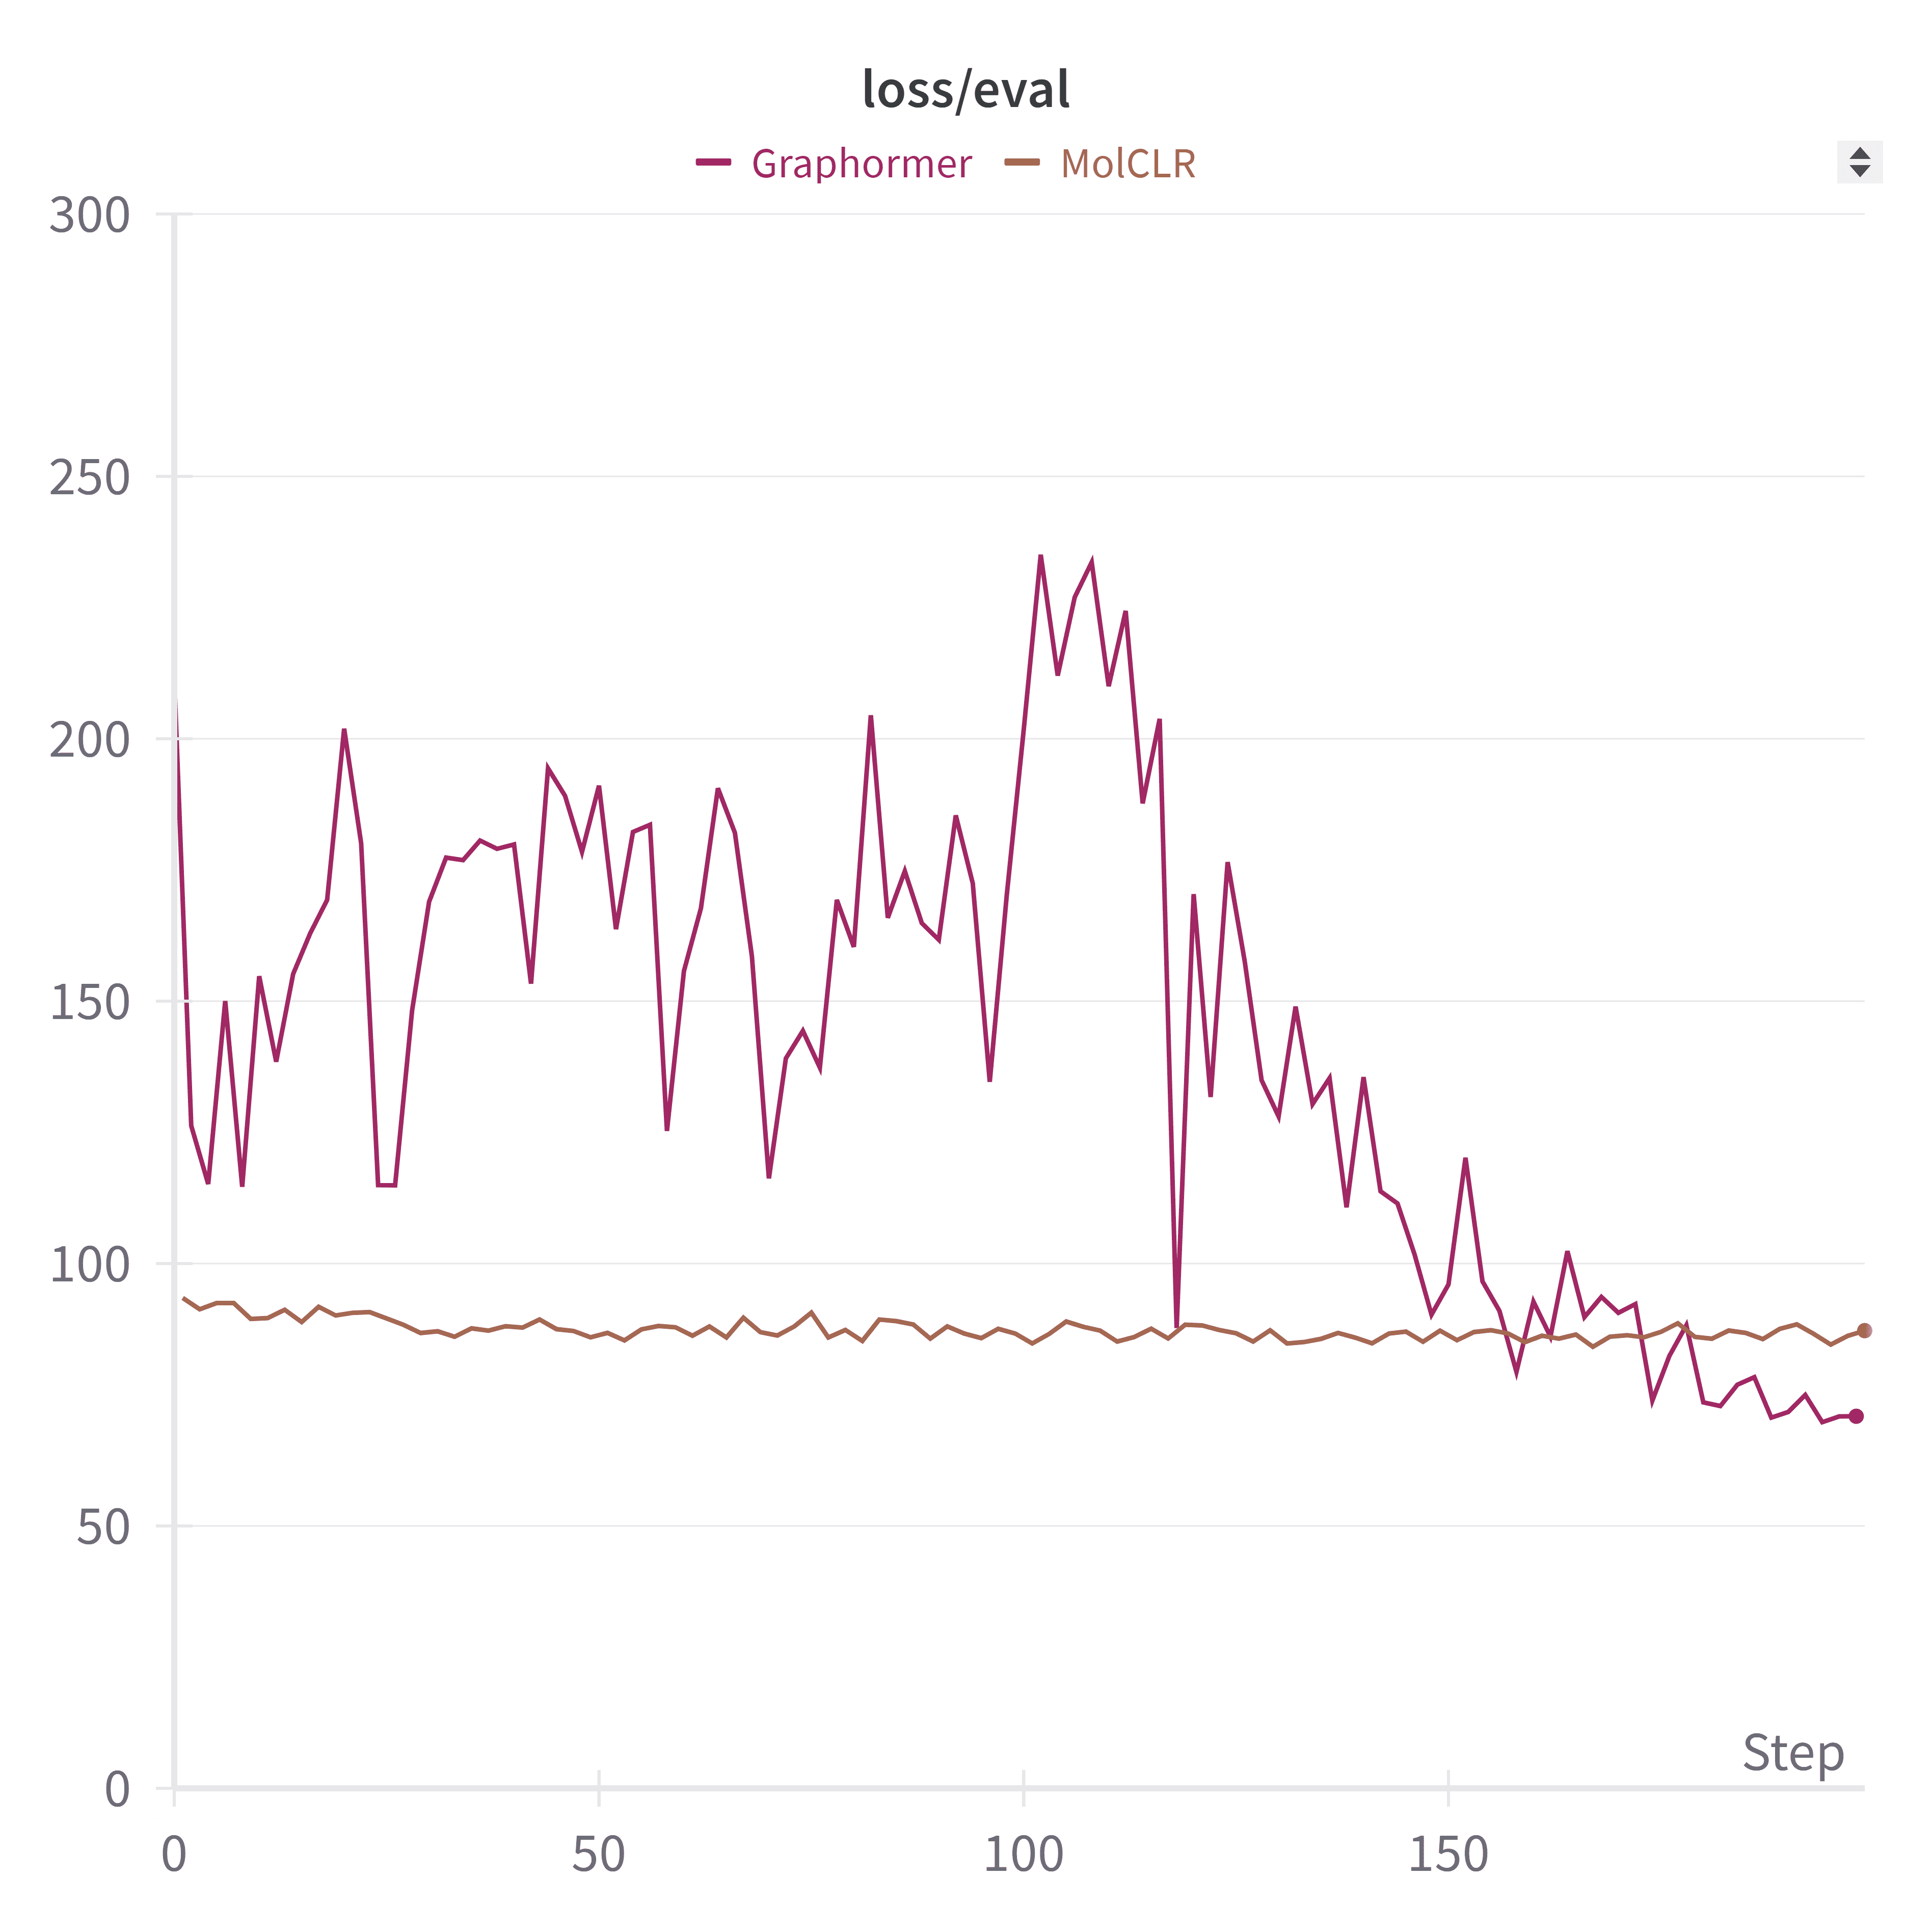
\includegraphics[width =  \textwidth ]{Bachelor-Thesis-Template/images/graphormer/eval_graphormer.png}
    \end{minipage}%

    \newline
    \begin{minipage}{0.5\textwidth}
      \centering
    \textbf{(a)}
    \end{minipage}%
    \begin{minipage}{0.5\textwidth}
    \centering
    \textbf{(b)}
    \end{minipage}%
    
    \caption{\small Сравнение графиков функций потерь Graphormer и MolCLR: (a) train, (b) validation}
    \label{fig:graphormer_vs_molclr_loss}
\end{figure}

\subsection{Разработка и реализация baseline-модели}
В данном разделе будет рассмотрен подход к обучению двух моделей на основе разных представлений молекулярных данных. В качестве отправной точки, или “бейзлайна”, были выбраны две модели: RoBERTa \cite{liu2019roberta} и MolCLR \cite{molclr}. Эти модели были выбраны из-за их эффективности в обработке текстовых и графовых данных соответственно, а также из-за относительной простоты их объединения. Для приближения эмбеддингов, полученных от каждой из этих моделей, использовалась функция косинусоидальной близости CosineSimilarityLoss. Обучение проводилось на датасете ChemBL. \cite{ChemBL}
Общая схема модели изображена на рисунке \ref{fig:bert_plus_molclr}.

\begin{figure}[h]
    \centering
    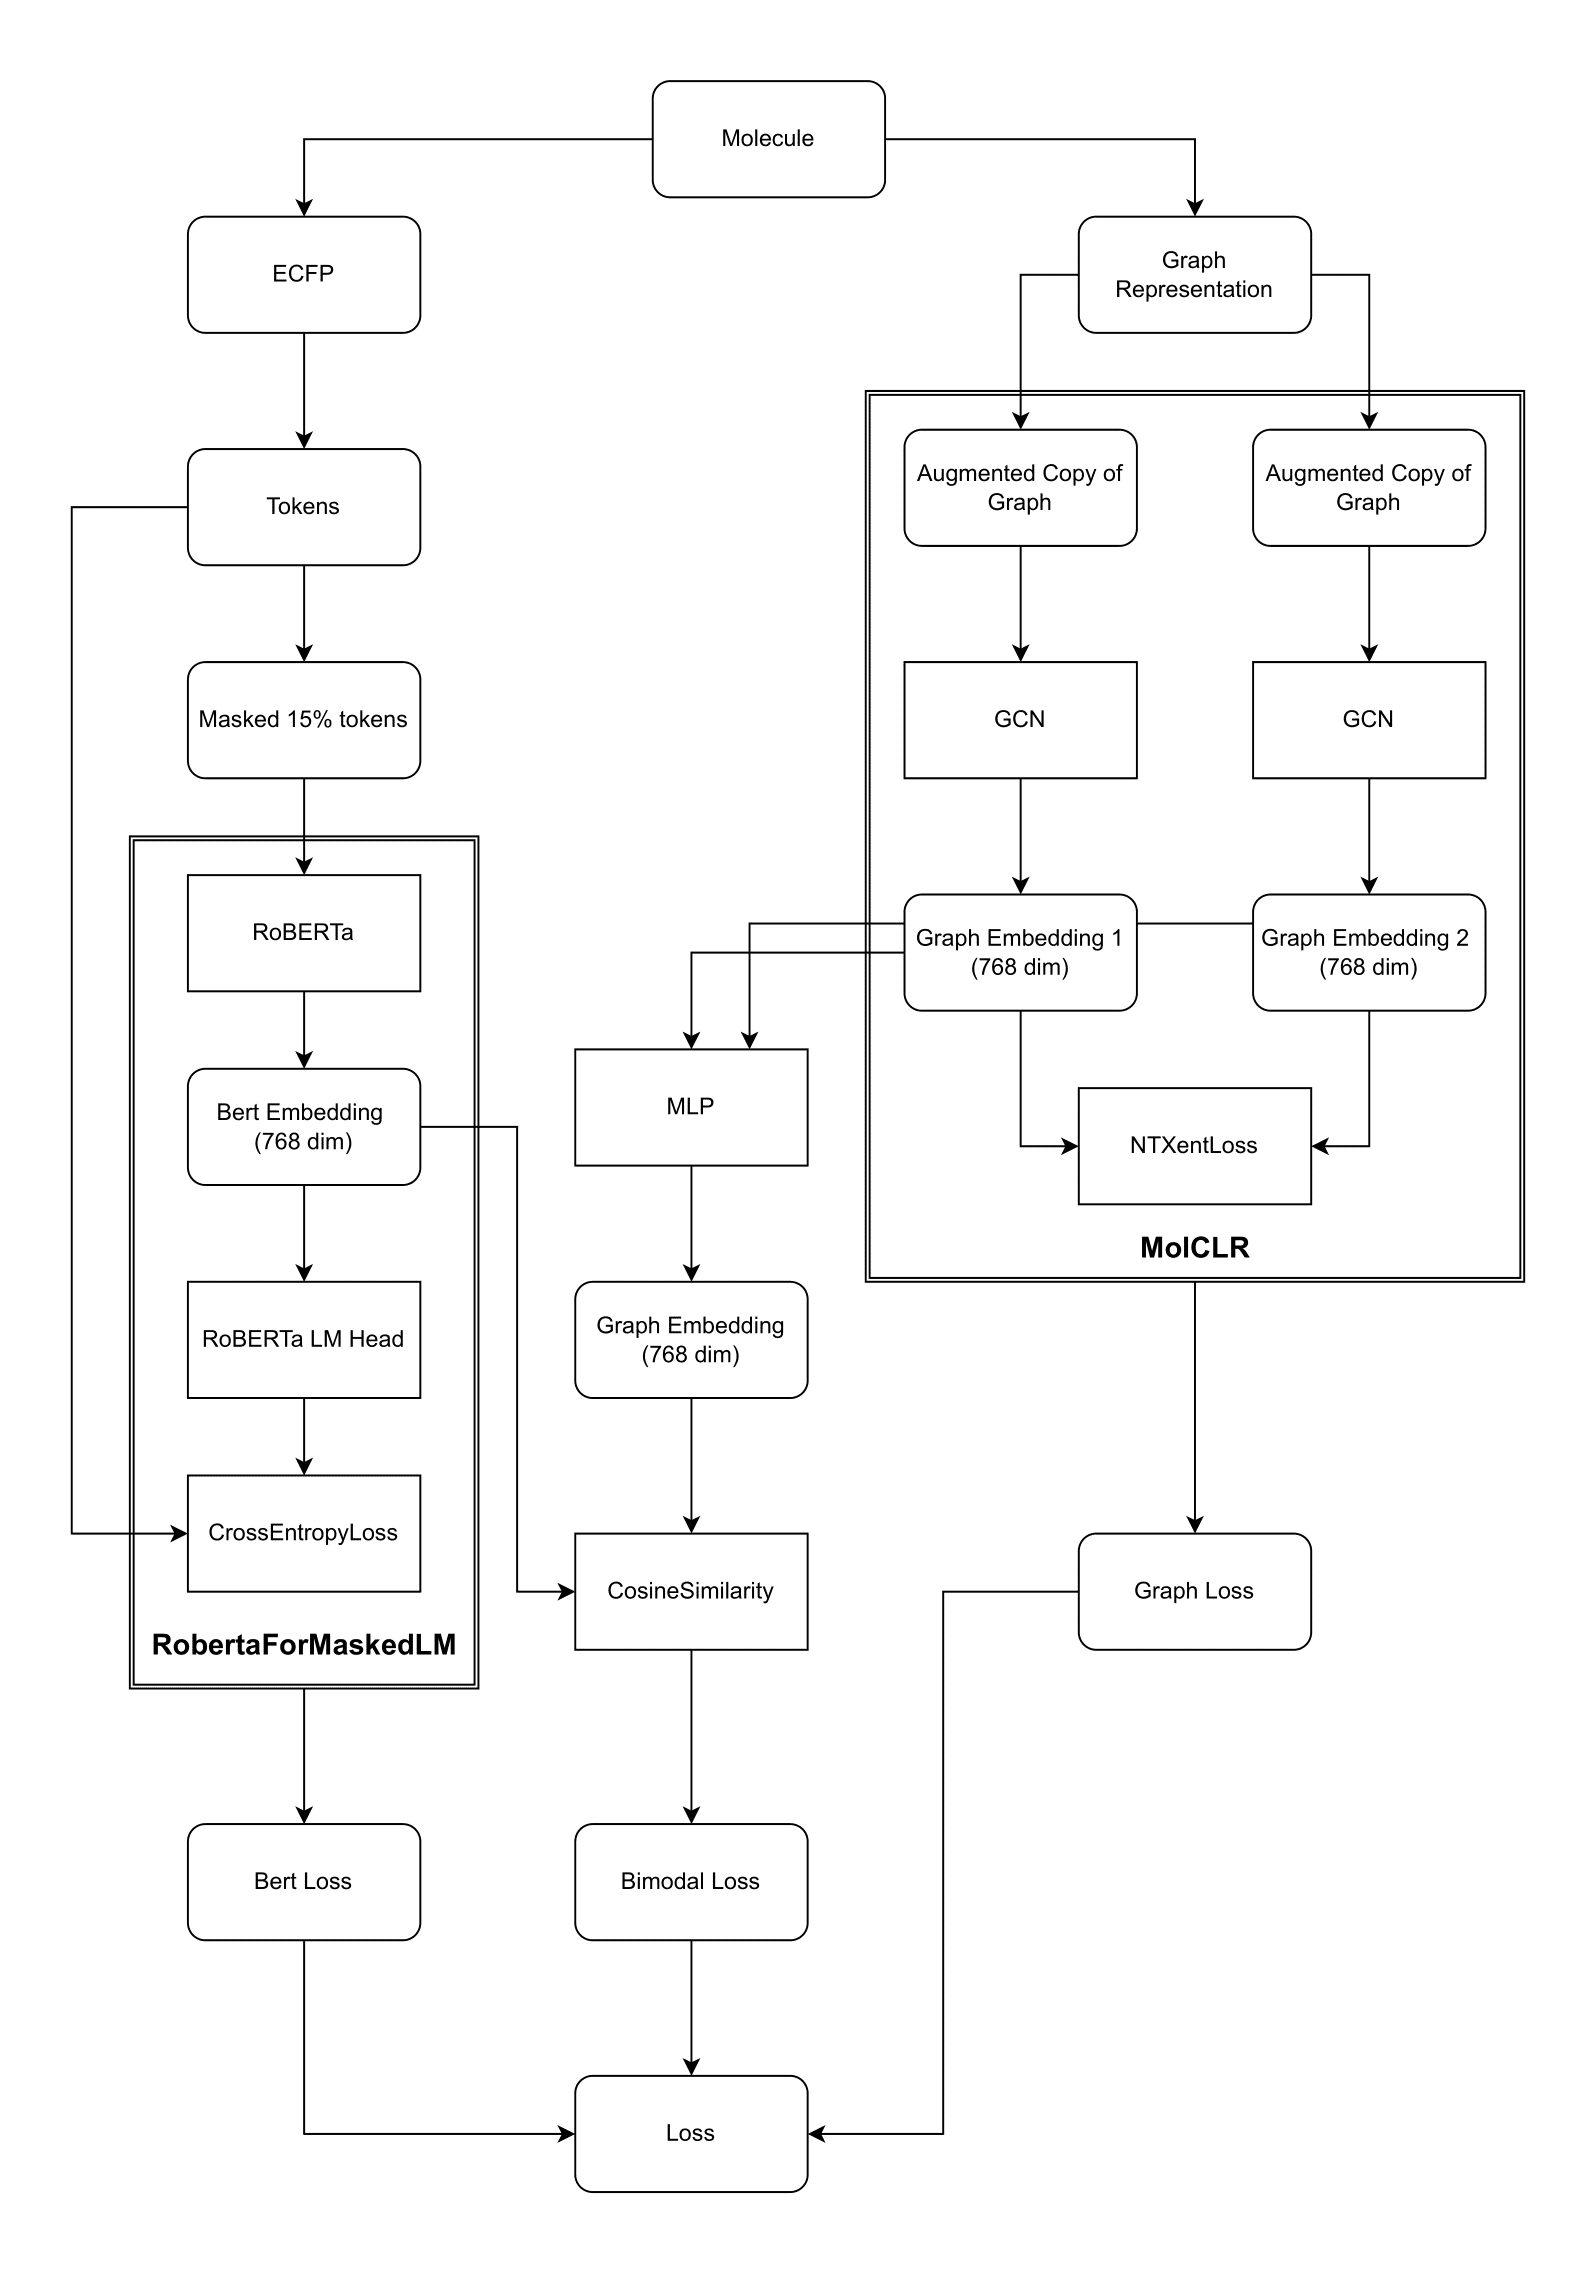
\includegraphics[width = 0.7 \textwidth ]{Bachelor-Thesis-Template/images/scheme.png}
    
    \caption{\small Архитектура объединения двух моделей RoBERTa и MolCLR.}
    \label{fig:bert_plus_molclr}
\end{figure}

\subsubsection{Описание алгоритма обучения}
\begin{enumerate}
    \item Инициализация класса MoleculeDataset, который наследуется от класса Dataset из библиотеки \texttt{torch\_geometric} и предназначен для создания набора данных из молекулярных структур, представленных в формате SMILES. Полученный набор данных состоит из токенов для входа модели трансформера, а также двух графовых представлений одной молекулы, которое используется в MoLCLR. Токены получаются применением вышеопределенных функций \texttt{tokenize} и \texttt{mlm}. Графовые представления являются агментированными копиями графа молекулы. 
    Метод класса MoleculeDataset \texttt{\_\_getitem\_\_}:
    \begin{lstlisting}
def __getitem__(self, index):
    node_feat, edge_index, edge_attr, num_nodes, num_edges = self.get_graph_from_smiles(self.dataset['Smiles'][index])

    graph_i = self.get_augmented_graph_copy(node_feat, edge_index, edge_attr, num_nodes, num_edges)
    graph_j = self.get_augmented_graph_copy(node_feat, edge_index, edge_attr, num_nodes, num_edges)

    ecfp = self.dataset['ecfp1'][index]
    data_for_bert = self.apply_mlm(self.tokenize(ecfp))
    return data_for_bert, graph_i, graph_j
    \end{lstlisting}
    \item Инициализация класса MolecularBertGraph: Этот класс представляет собой модель, которая объединяет модель \texttt{RobertaForMaskedLM} и графовую нейронную сеть MolCLR:
    \begin{lstlisting}
from transformers import RobertaForMaskedLM
from transformers import RobertaConfig

if config['model_type'] == 'gin':
    from MolCLR.models.ginet_molclr import GINet as GraphModel
elif config['model_type'] == 'gcn':
    from MolCLR.models.gcn_molclr import GCN as GraphModel
else:
    raise ValueError('GNN model is not defined in config.')
from MolCLR.utils.nt_xent import NTXentLoss

class MolecularBertGraph(torch.nn.Module):
    def __init__(self):
        super(MolecularBertGraph, self).__init__()
        self.bert = RobertaForMaskedLM(roberta_config)
        self.graph_model = GraphModel(**config['model'])
        self.out_graph_linear = torch.nn.Linear(768 * 2, 768, bias=True)
        # contrastive loss for MolCLR
        self.nt_xent_criterion = NTXentLoss(self.batch_size, **config['loss'])
        # cosine distance as loss between models
        self.cosine_sim = torch.nn.CosineSimilarity(dim=-1)

    def forward(self, bert_batch, graph_batch1, graph_batch2):
        bert_output = self.bert(bert_batch)
        bert_loss = bert_output.loss
        bert_emb = bert_output.hidden_states[0][:, 0, :] # CLS embedding 

        graph_loss, hidden_states_1, hidden_states_2 = self.graph_step(graph_batch1, graph_batch2)
        graph_emb = self.out_graph_linear(torch.cat((hidden_states_1, hidden_states_2), dim=-1))

        bimodal_loss = ((1 - self.cosine_sim(bert_emb, graph_emb))**2).mean()
        return bert_loss, graph_loss, bimodal_loss

    def graph_step(self, xis, xjs):
        ris, zis = self.graph_model(xis)
        rjs, zjs = self.graph_model(xjs)
        # normalize projection feature vectors
        zis = torch.nn.functional.normalize(zis, dim=1)
        zjs = torch.nn.functional.normalize(zjs, dim=1)
        
        loss = self.nt_xent_criterion(zis, zjs)
        return loss, ris, rjs
    \end{lstlisting}
    \item Cоздание экземпляра MoleculeDataset, загрузчиков данных для обучающего и валидационного наборов данных, а также экземпляра MolecularBertGraph.
    \item Инициализация стандартного оптимизиматора AdamW с lr равным 5e-3.
    \item В цикле обучения вычисляется значения функции потерь \texttt{bert\_loss}, \texttt{graph\_loss}, \texttt{bimodal\_loss} на каждом батче из \texttt{train\_dataloader}. Финальное значение функции потерь вычисляется по формуле 
    
    $$\texttt{loss} = \alpha * \texttt{bert\_loss} + \beta * \texttt{graph\_loss} + \gamma * \texttt{bimodal\_loss}$$ 
    
    где $\alpha$, $\beta$, $\gamma$ - соответсвующие коэффиценты (гиперпараметры). Далее происходит обратное распространение ошибки. Результатом одной эпохи было усреднение всех значений функции потерь по всей эпохе.

    \item В цикле валидации \texttt{eval\_loop()} был выполнен проход по каждому батчу в валидационном \texttt{eval\_dataloader}. Процесс был аналогичен циклу обучения, однако в этом случае веса модели не обновлялись. Валидация происходила каждую эпоху.
    
    \item Далее идет основной цикл обучения, который выполняет заданное количество эпох обучения. В каждой эпохе выполняются обучающий и валидационный циклы, а также обновляются логи и сохраняются веса модели.

\end{enumerate}
В следующем разделе представлены графики обучения и валидации для всех четырех функций потерь: \texttt{bert\_loss}, \texttt{graph\_loss}, \texttt{bimodal\_loss} и \texttt{loss}. Эти графики помогут лучше понять динамику обучения и валидации модели, а также влияние каждой из компонент потери на общую функцию потерь.

\subsubsection{Результаты baseline-эксперимента}
Baseline эксперимент был проведен с двумя вариантами графовых моделей: GCN и GIN.
На рисунке \ref{fig:loss_bimodal} представлен график динамики общей функции потерь для двух моделей: RobertaForMaskedLM + MolCLR (GIN) и RobertaForMaskedLM + MolCLR (GCN) в процессе обучения (a) и в процессе валидации (b). Ось абсцисс представляет собой количество эпох обучения, а ось ординат - значения функции потерь, варьирующиеся от 0 до 1.

\begin{figure}[h]
    \begin{minipage}{0.5\textwidth}
        \centering
        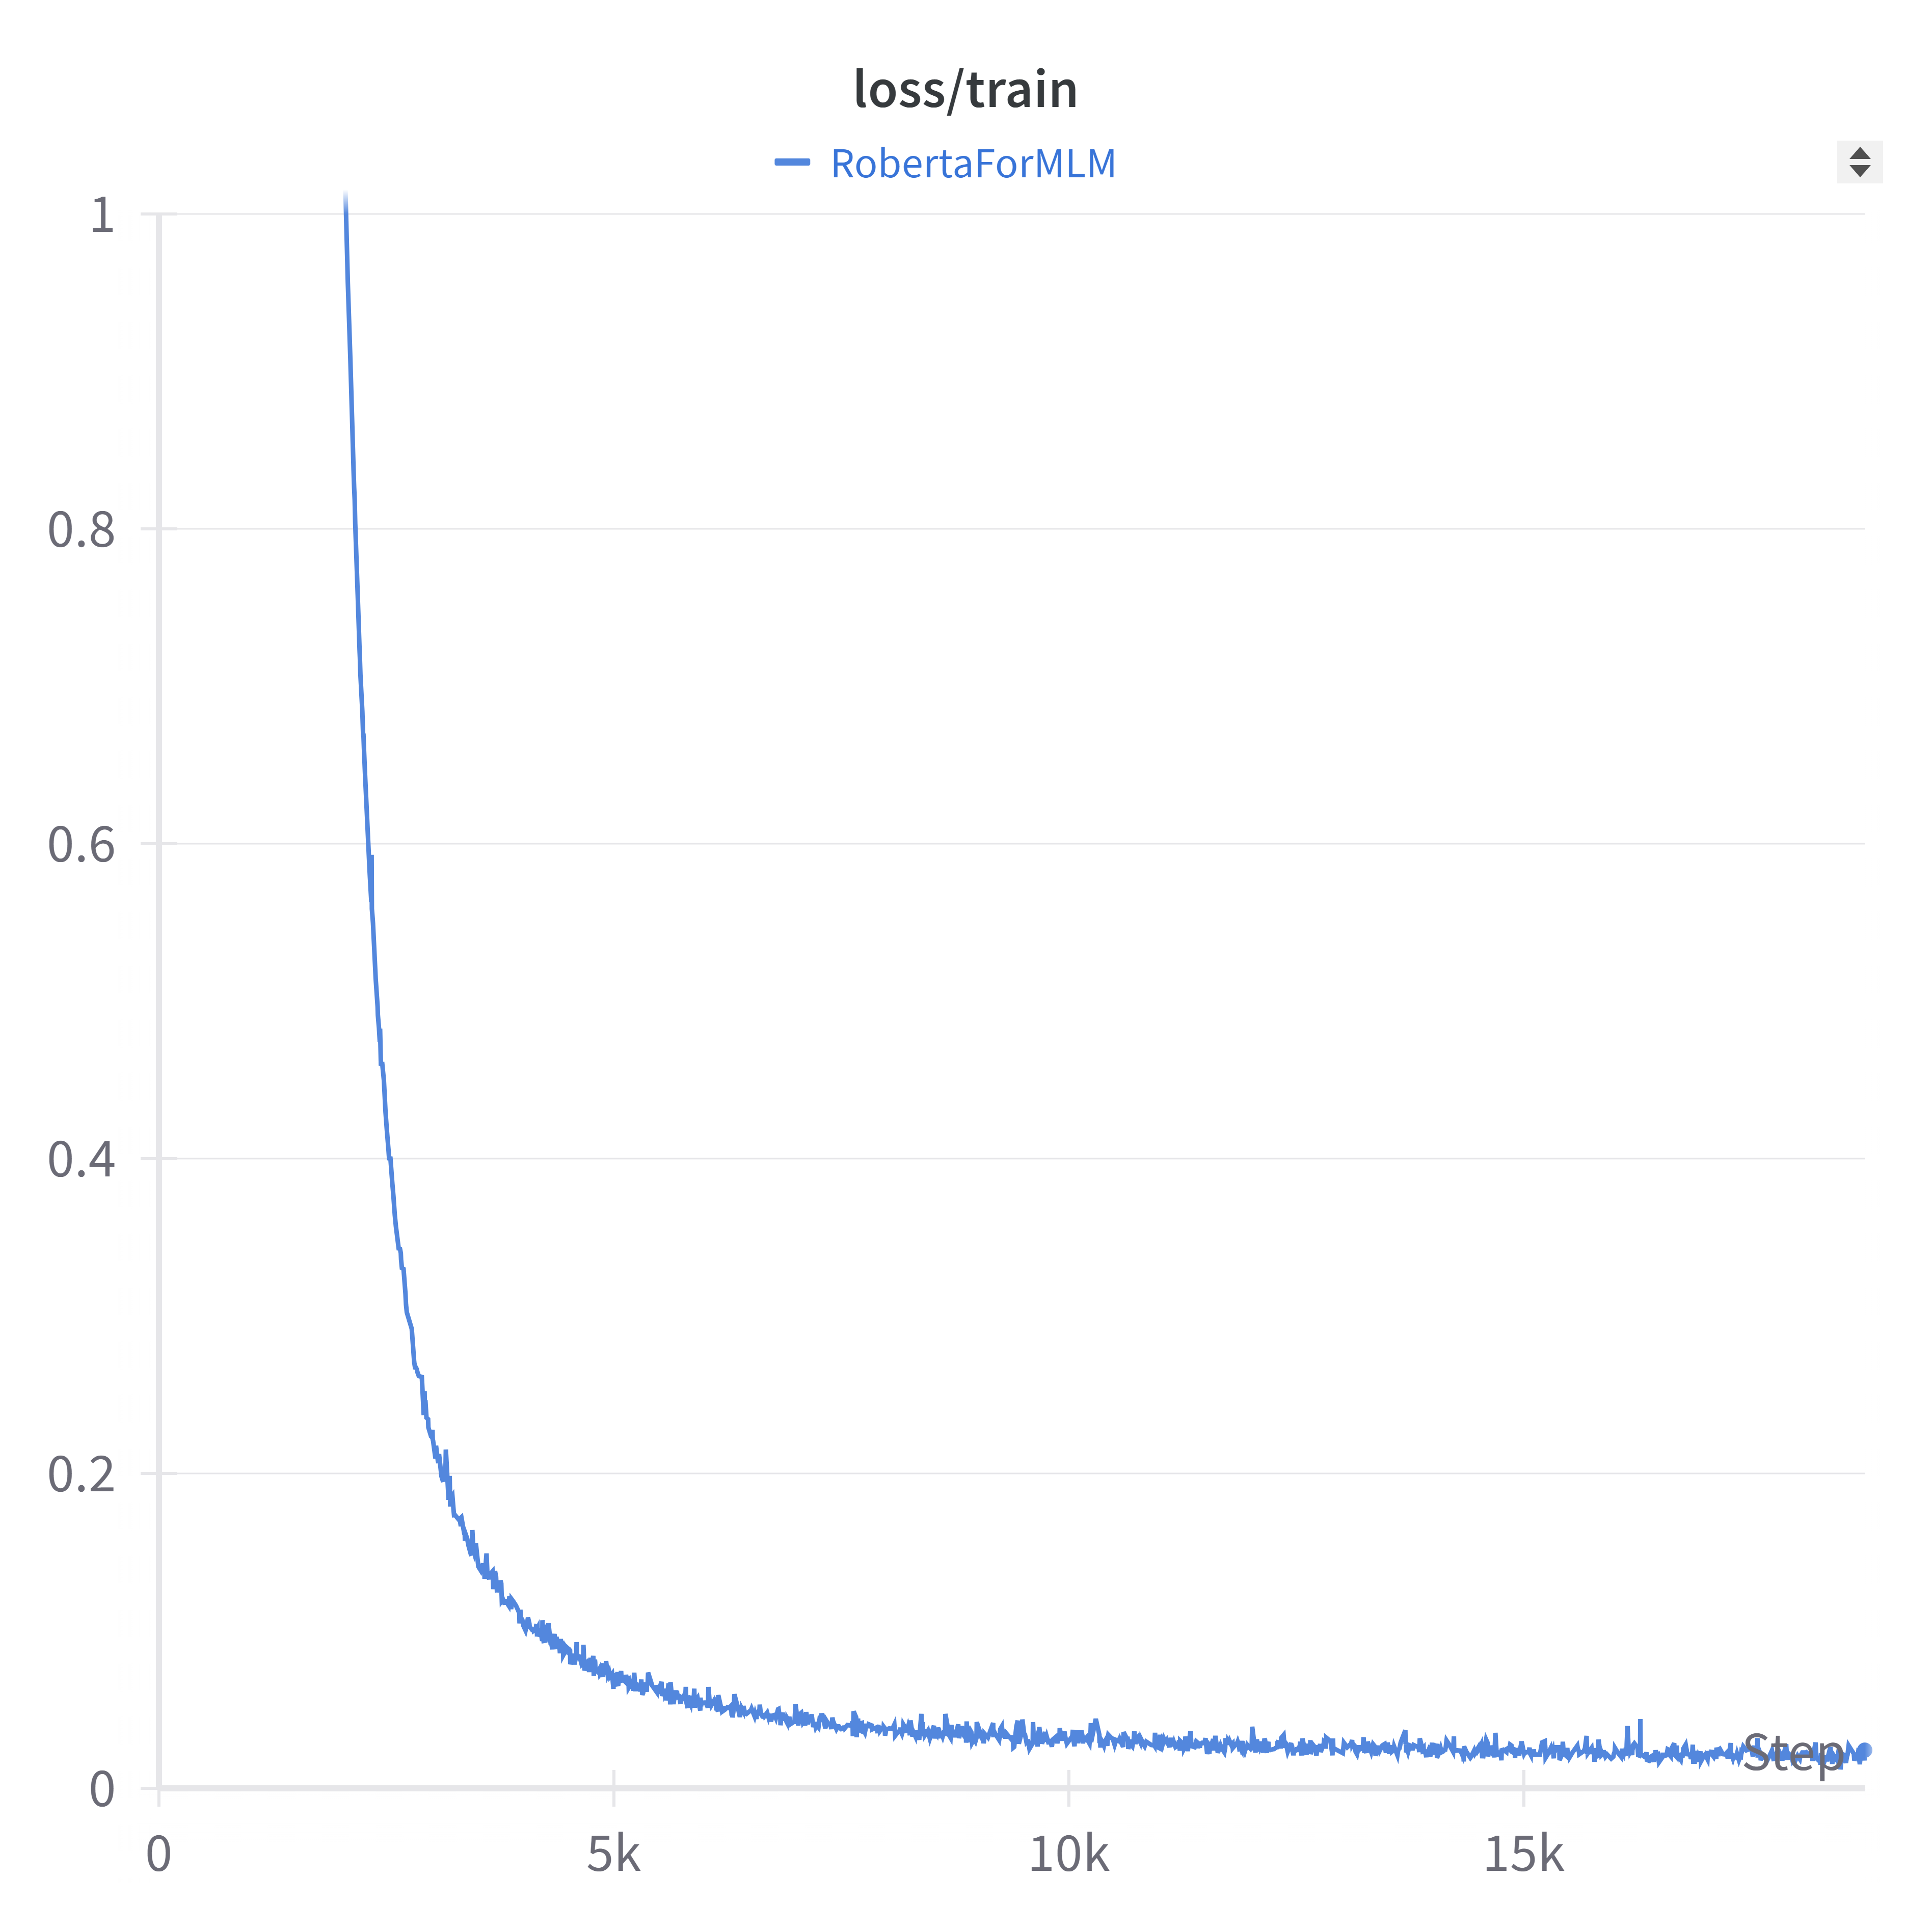
\includegraphics[width =  \textwidth ]{Bachelor-Thesis-Template/images/roberta_molclr/loss_train.png}
    \end{minipage}%
    \begin{minipage}{0.5\textwidth}
        \centering
        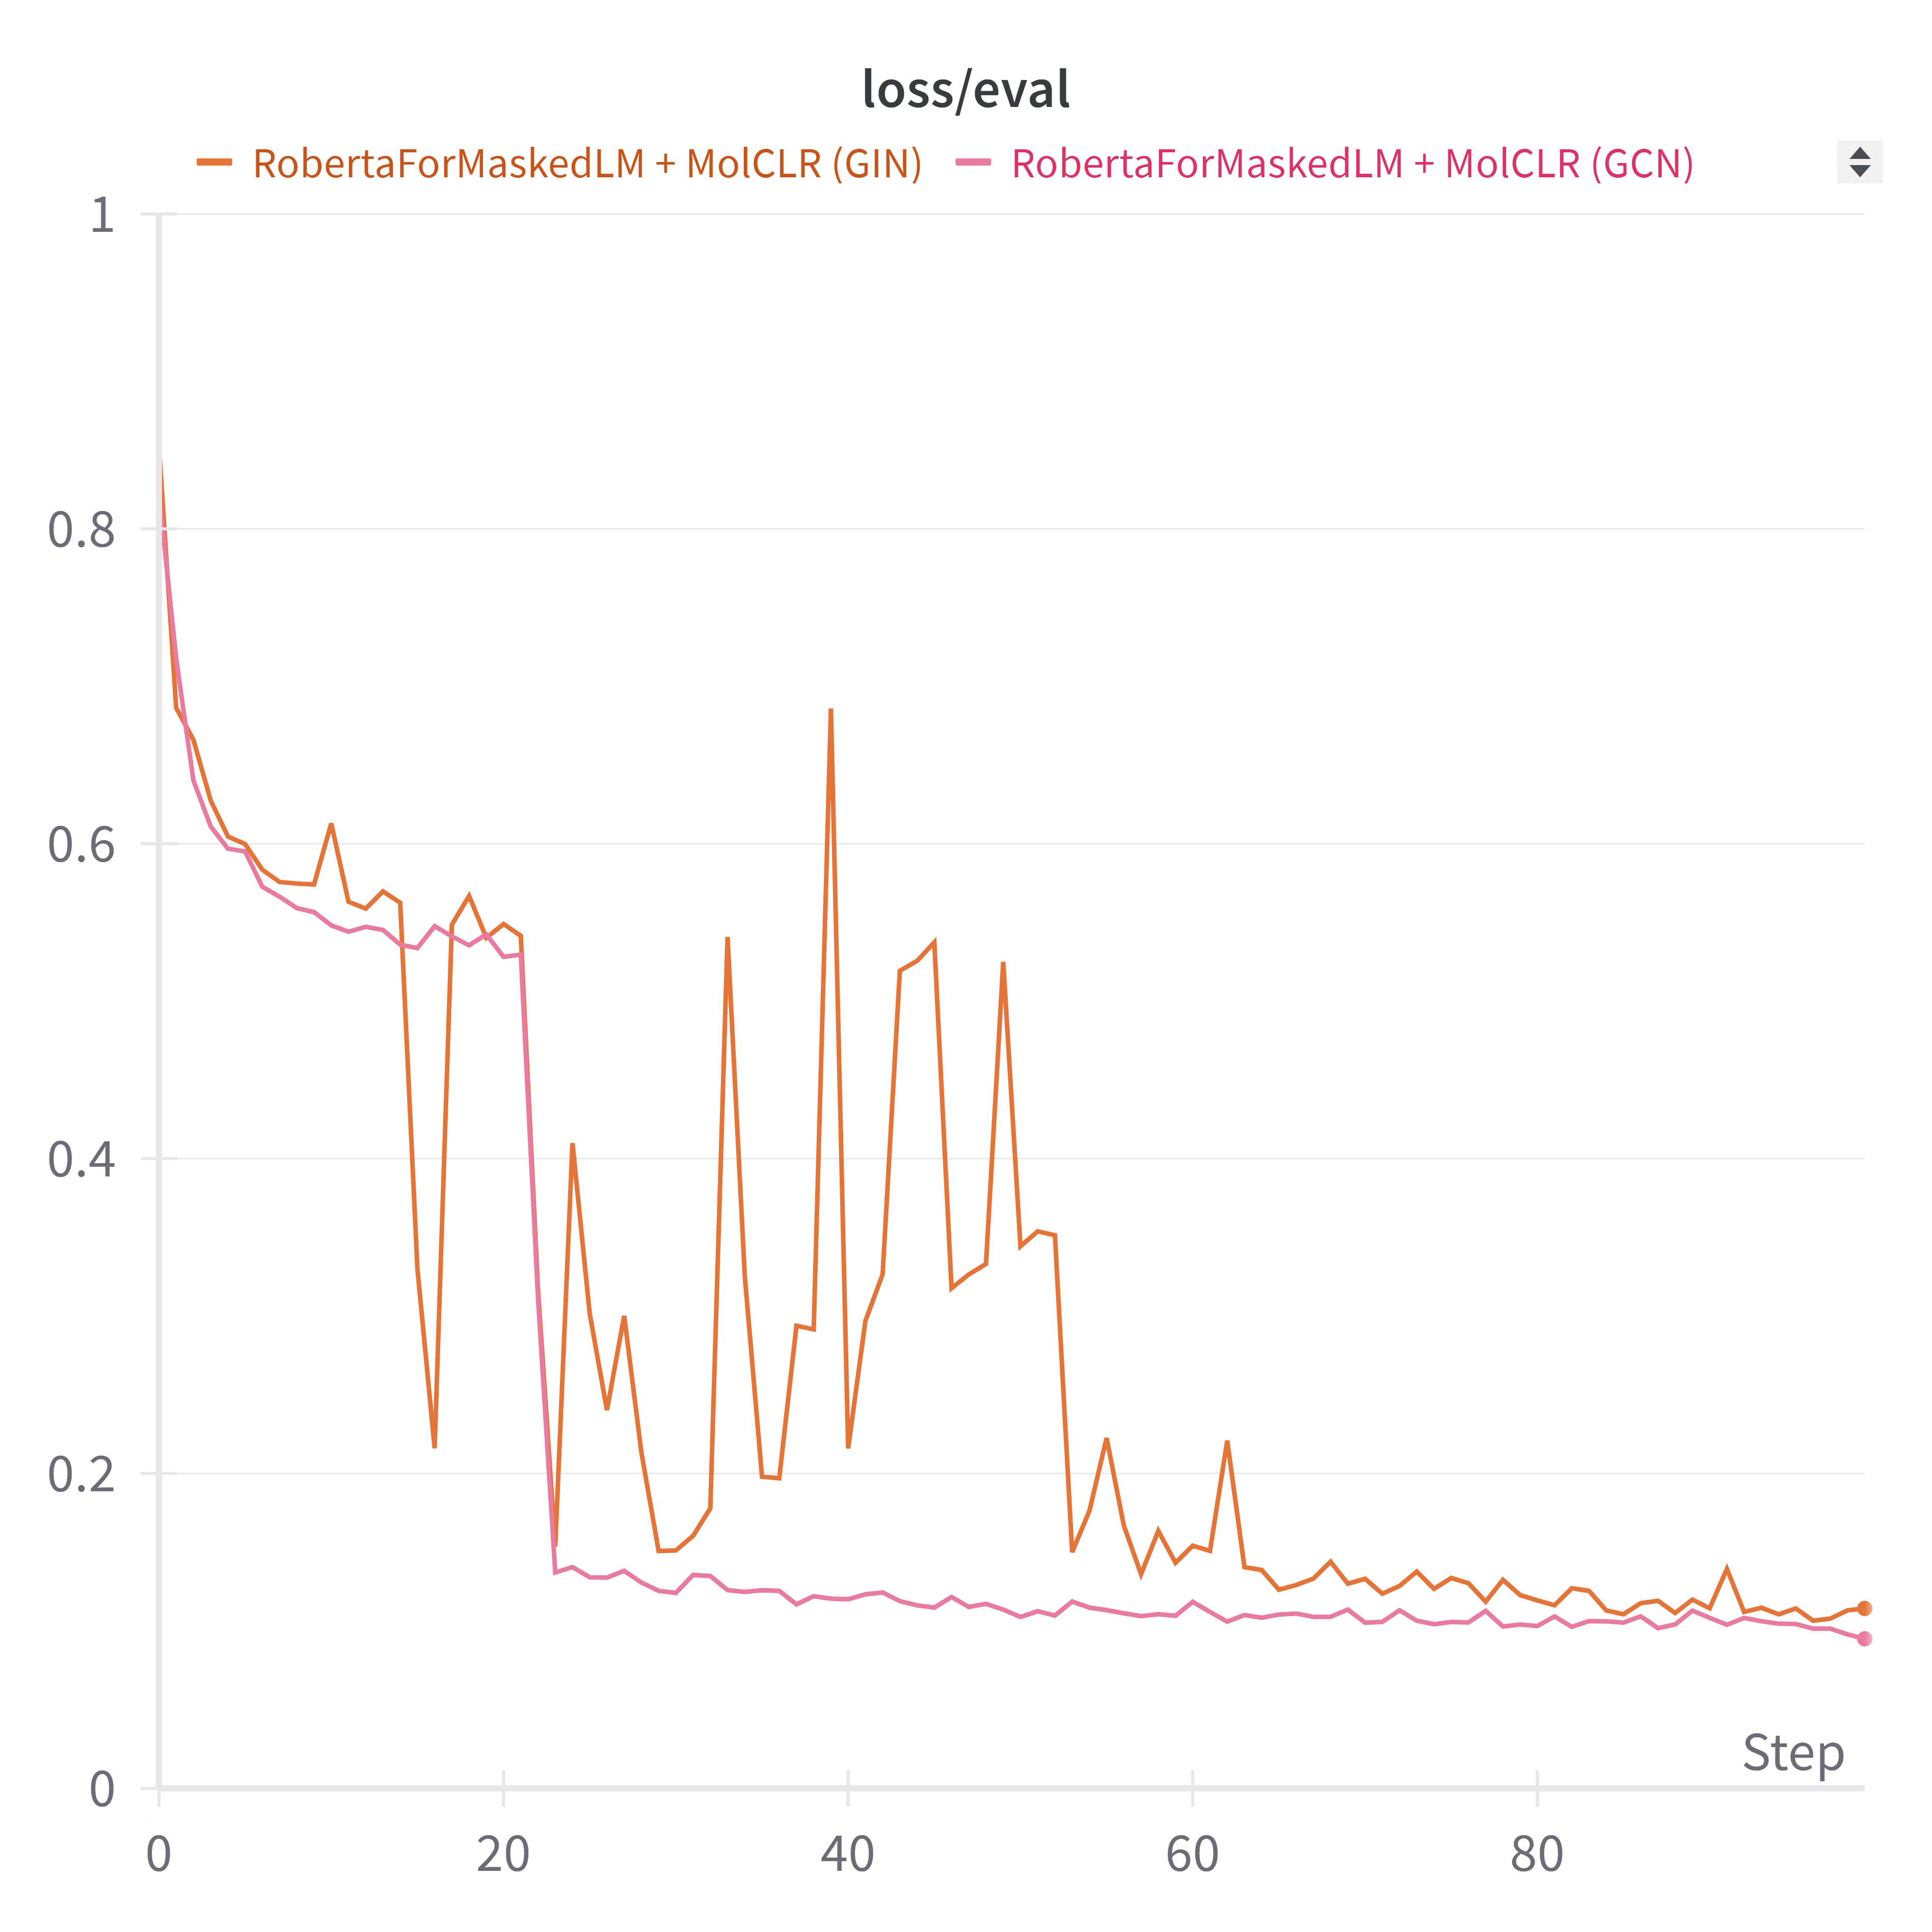
\includegraphics[width =  \textwidth ]{Bachelor-Thesis-Template/images/roberta_molclr/loss_eval.png}
    \end{minipage}%

    \newline
    \begin{minipage}{0.5\textwidth}
      \centering
    \textbf{(a)}
    \end{minipage}%
    \begin{minipage}{0.5\textwidth}
    \centering
    \textbf{(b)}
    \end{minipage}%
    
    \caption{\small Графики общей функций потерь в baseline-моделе: (a) train, (b) validation}
    \label{fig:loss_bimodal}
\end{figure}

Обе кривые на графике (a) рисунка \ref{fig:loss_bimodal} демонстрируют типичное поведение функции потерь в процессе обучения: быстрое уменьшение в начале, когда происходит основное обучение, за которым следуют более мелкие колебания и в конечном итоге стабилизация, по мере сходимости модели к оптимальным параметрам.

Красная линия, соотвествующая модели с графовой GIN, показывает резкое снижение потерь с начального значения в течение первых нескольких эпох, после чего следуют колебания с уменьшающейся амплитудой по мере продвижения вдоль шагов, в конечном итоге выравниваясь.

Оранжевая линия, соотвествующая модели с графовой GCN, также показывает начальное резкое снижение значений потерь, но с меньшими колебаниями по сравнению с красной линией, и далее она уменьшается более стабильно, приближаясь к своей асимптоте.

График валидации (b) демонстрирует аналогичные изменения для обоих конфигураций модели, что характеризует успешное проведение эксперимента и качественное обучение полученной модели.

Далее, на рисунках \ref{fig:roberta_loss_bimodal}, \ref{fig:molclr_loss_bimodal} и \ref{fig:bimodal_loss_bimodal} представлены графики функций потерь RoBERTa, MolCLR и бимодальной функции потерь в baseline-модели соответсвенно. Графики показаны при обучении модели (a) и при валидации (b), а также для двух вариантов графовой модели GCN и GIN. График междумодельной loss-функции отнормирован для наглядности.


\begin{figure}[h]
    \begin{minipage}{0.5\textwidth}
        \centering
        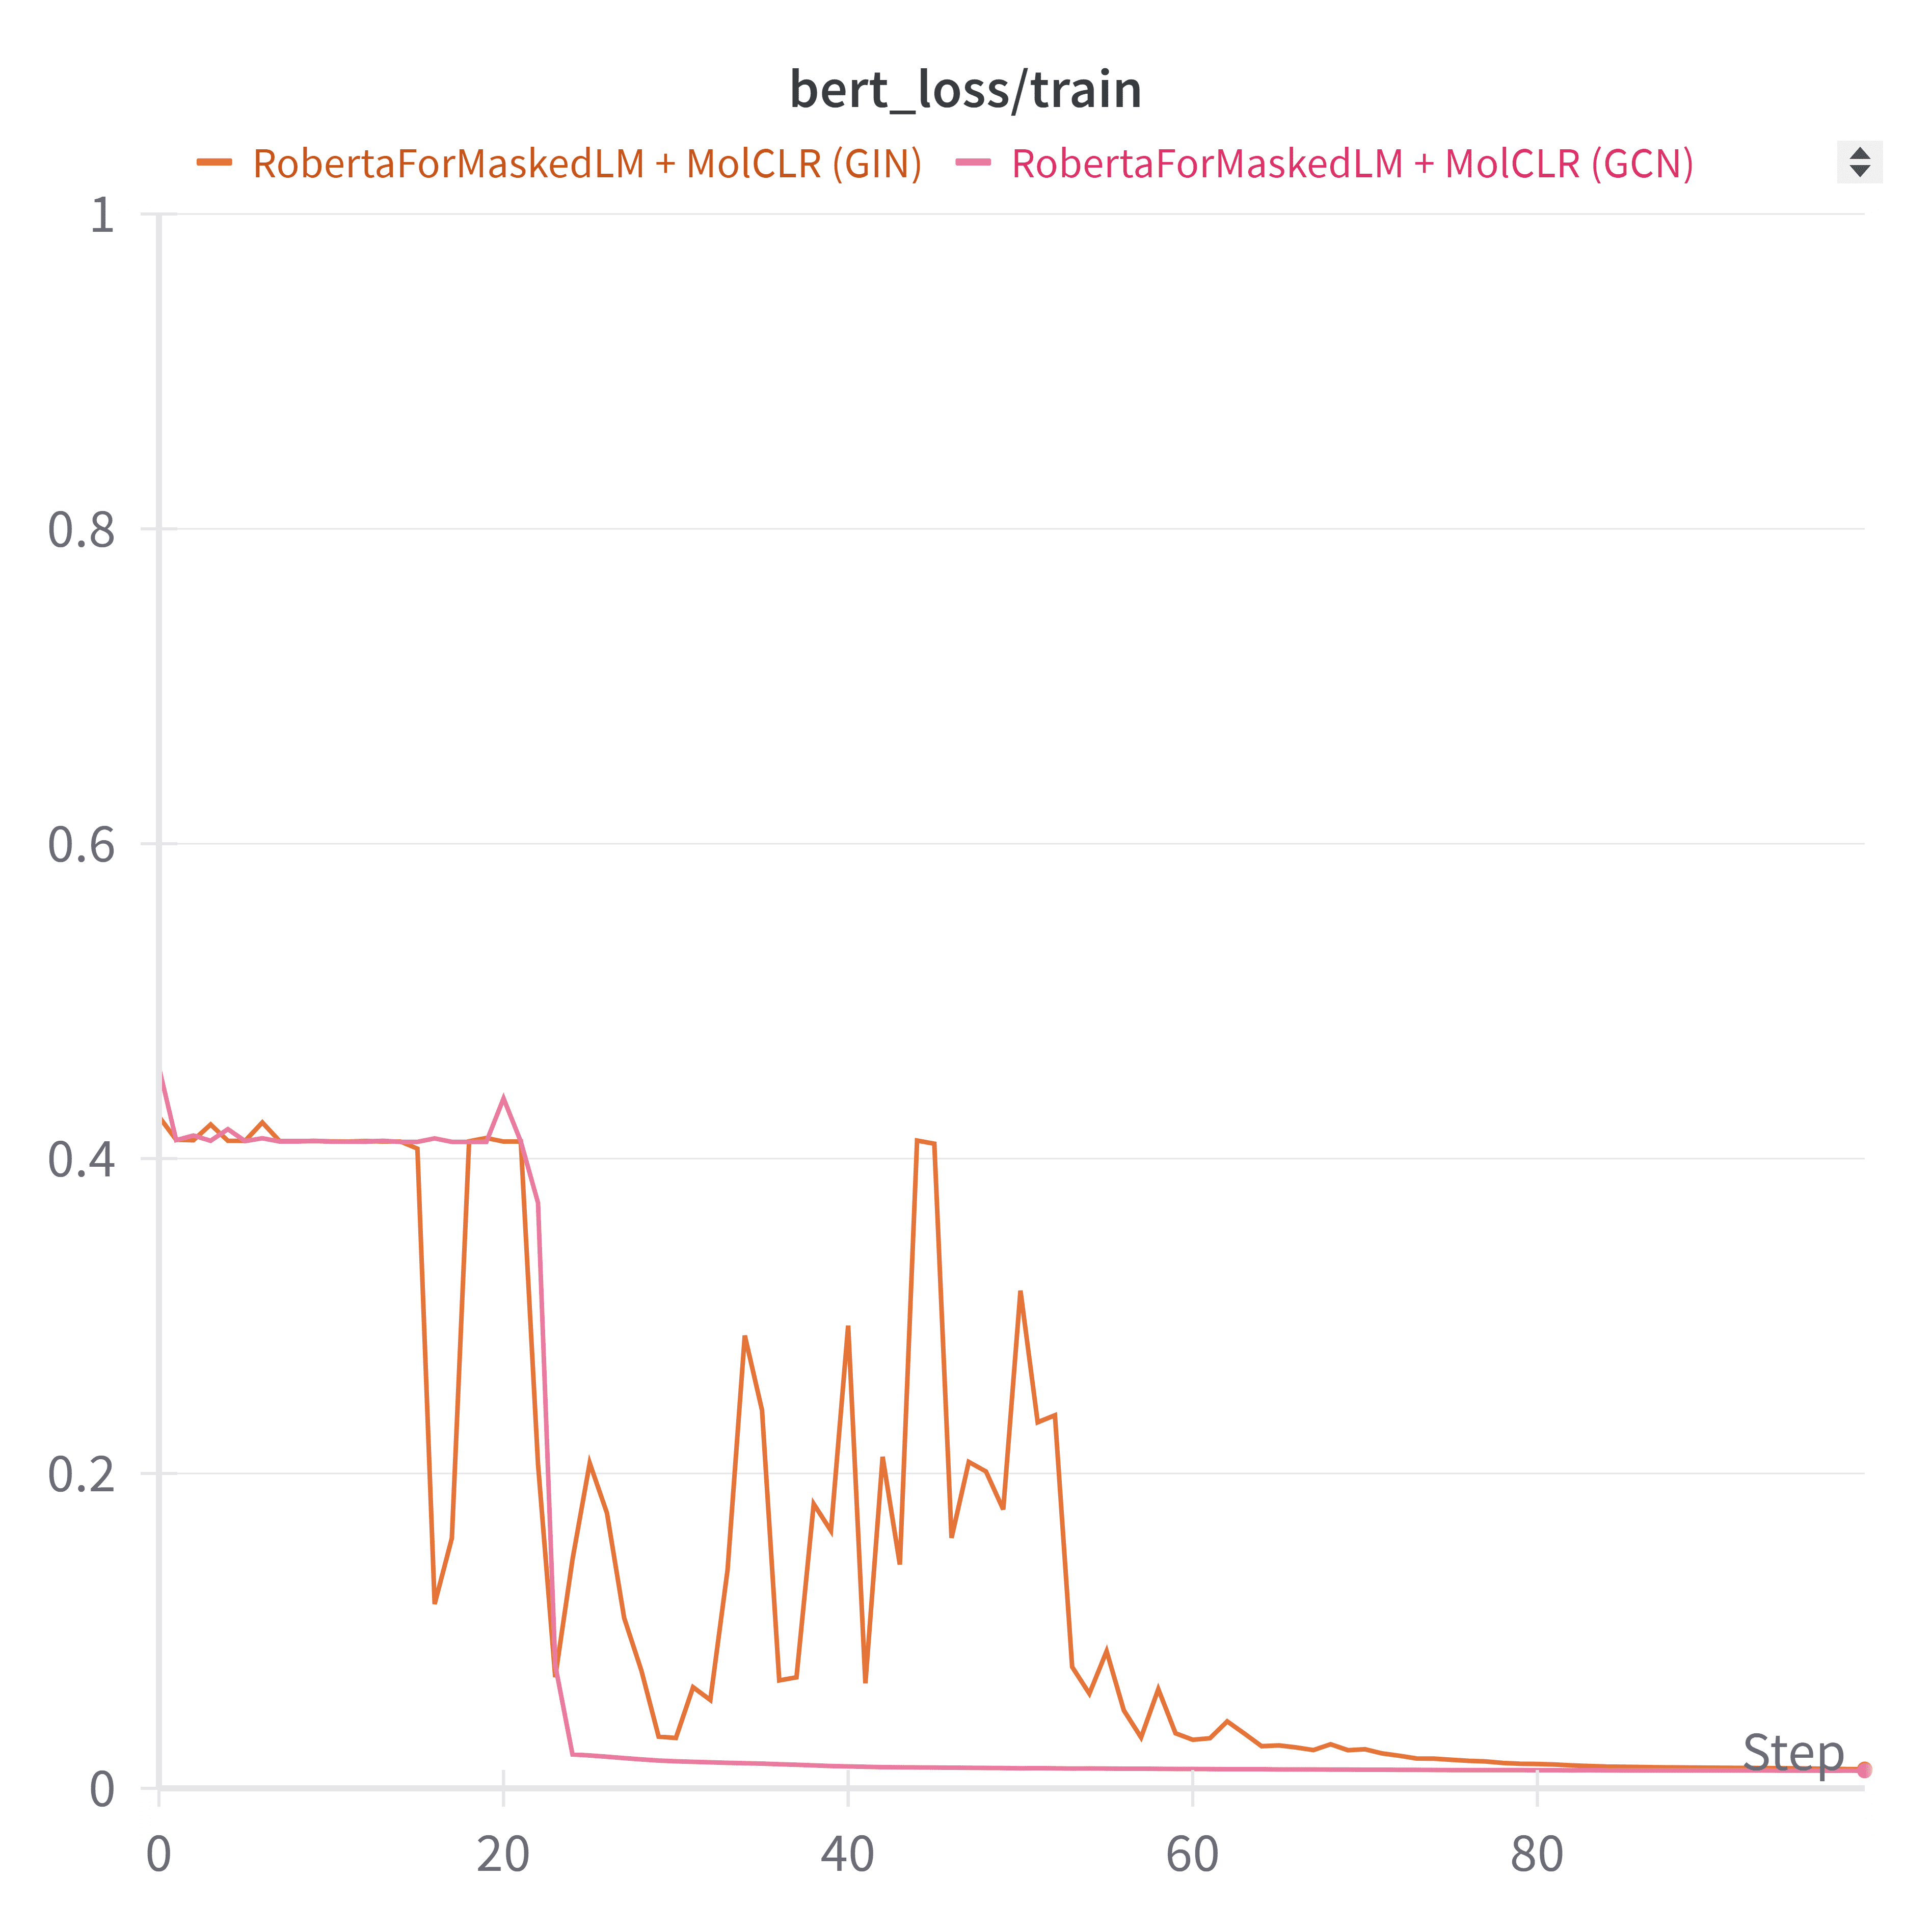
\includegraphics[width =  \textwidth ]{Bachelor-Thesis-Template/images/roberta_molclr/bert_loss_train.png}
    \end{minipage}%
    \begin{minipage}{0.5\textwidth}
        \centering
        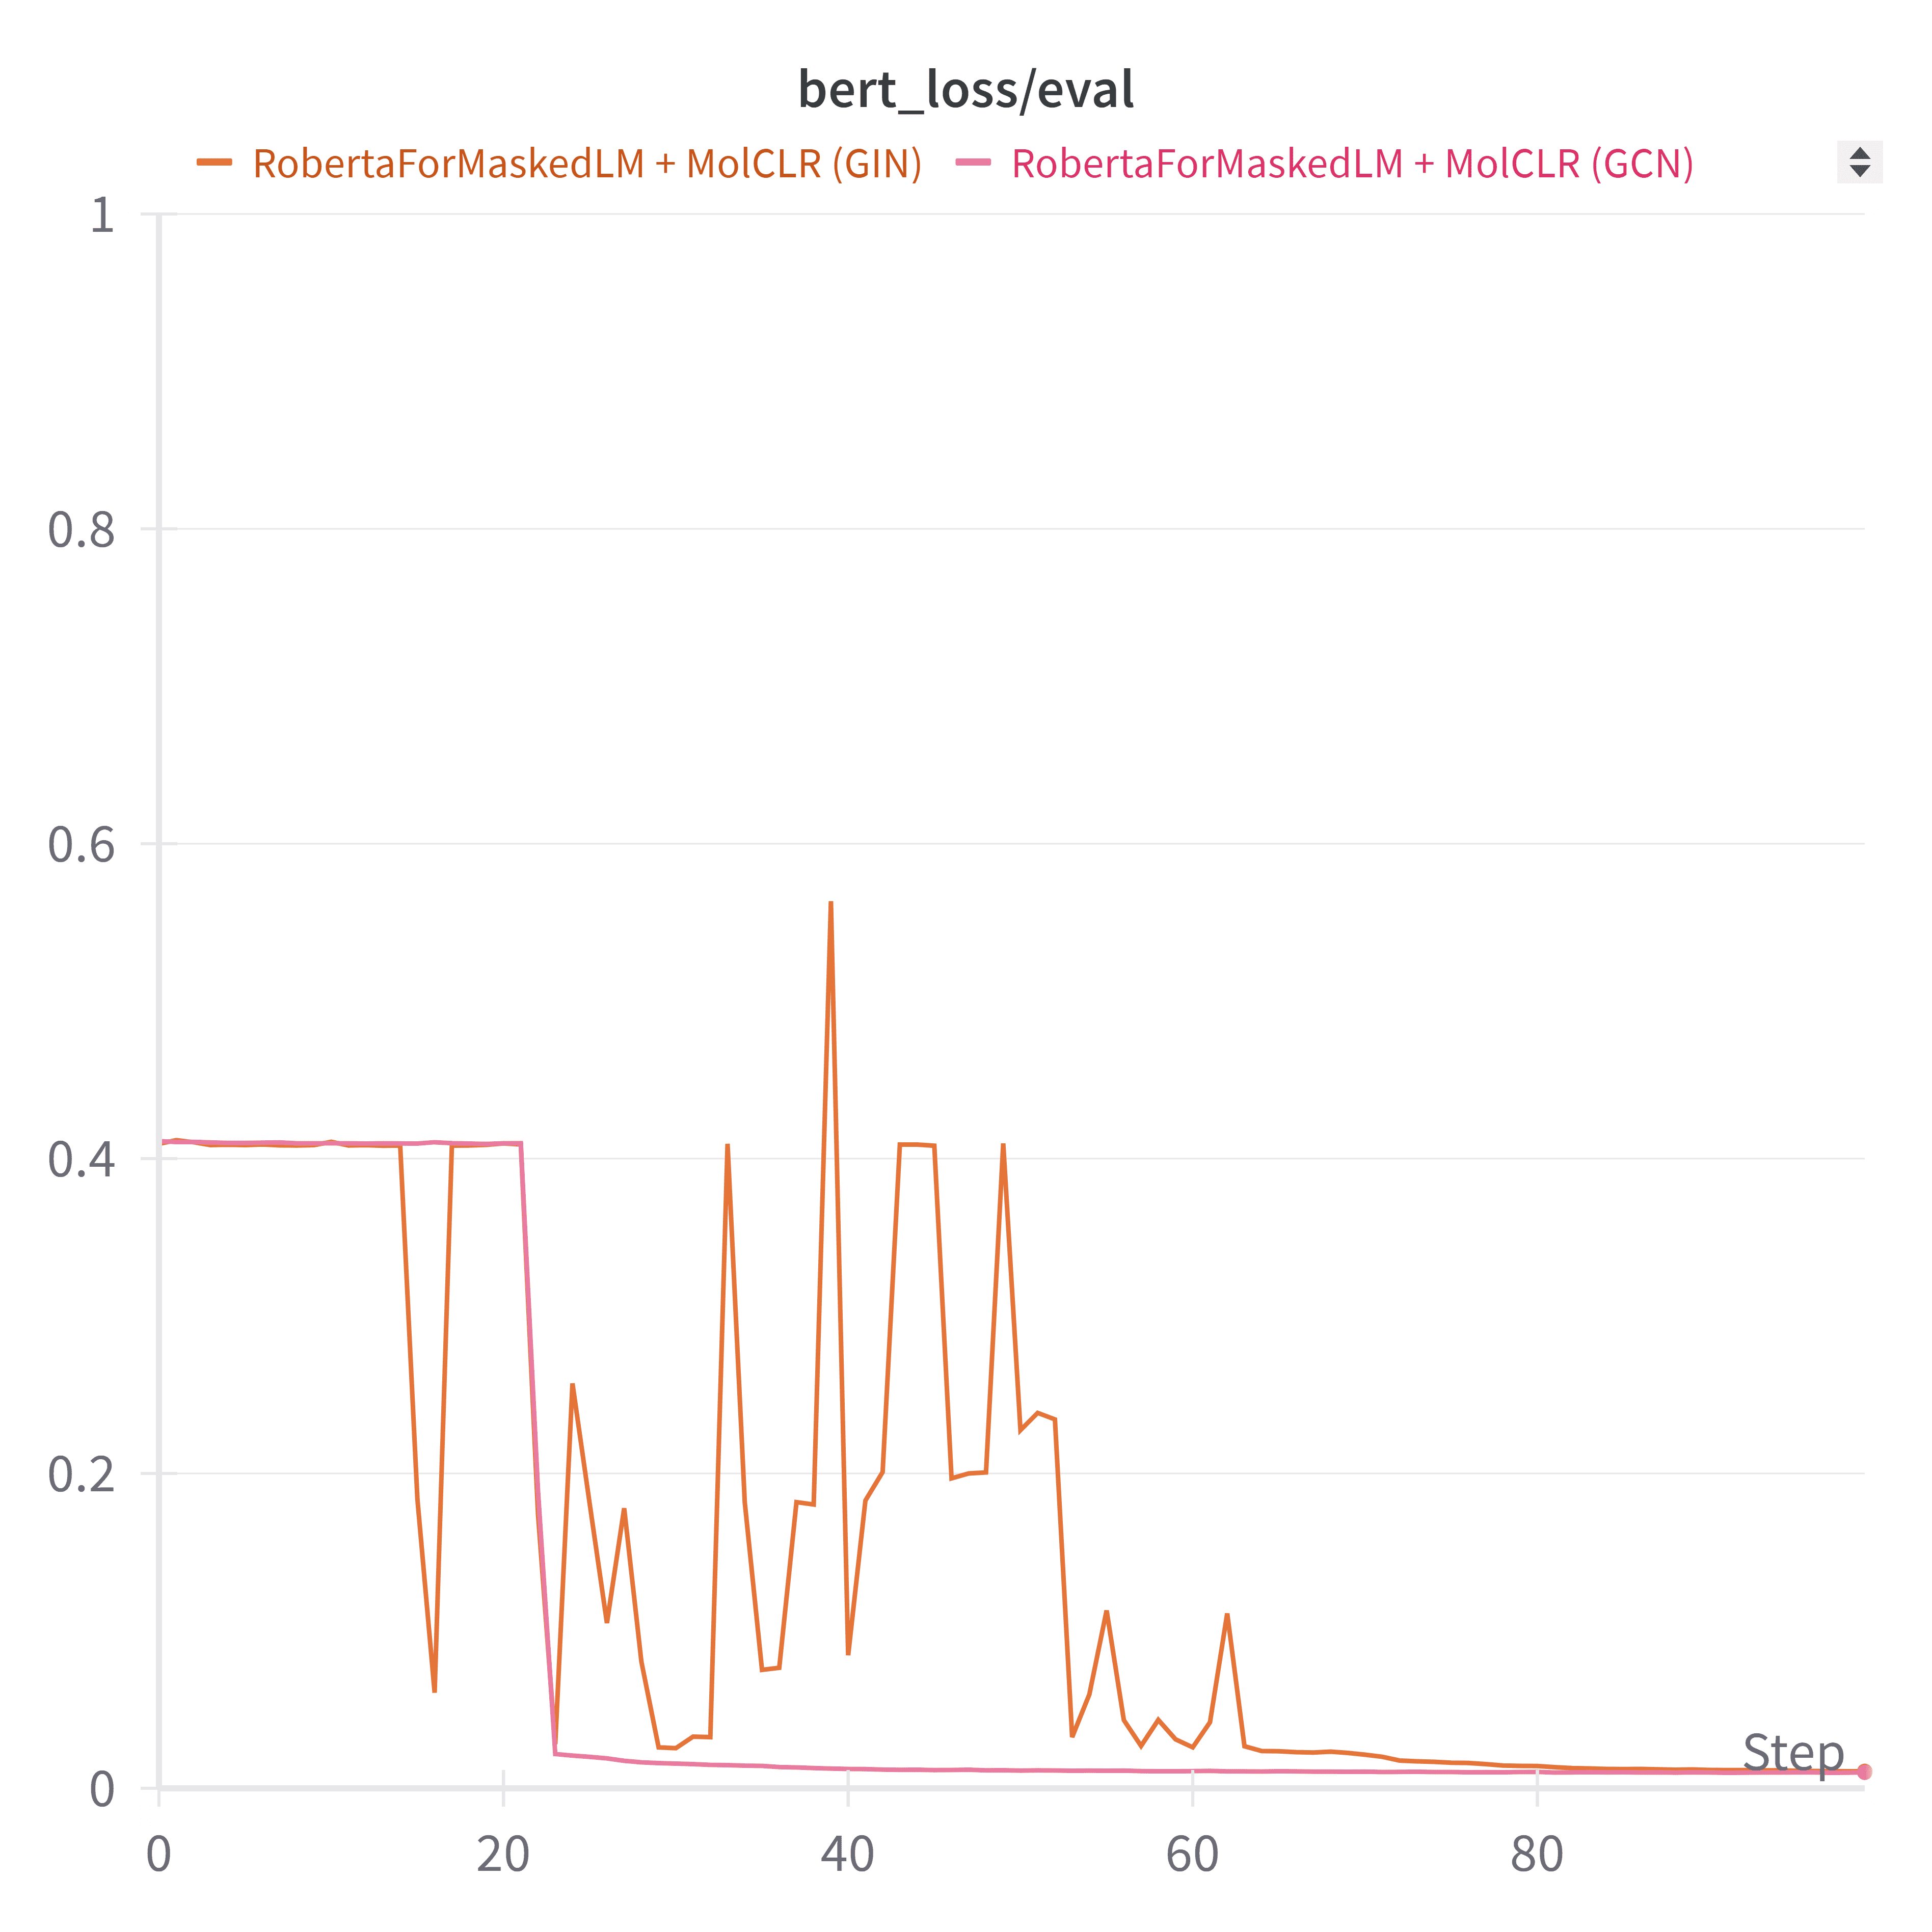
\includegraphics[width =  \textwidth ]{Bachelor-Thesis-Template/images/roberta_molclr/bert_loss_eval.png}
    \end{minipage}%

    \newline
    \begin{minipage}{0.5\textwidth}
      \centering
    \textbf{(a)}
    \end{minipage}%
    \begin{minipage}{0.5\textwidth}
    \centering
    \textbf{(b)}
    \end{minipage}%
    
    \caption{\small Графики функций потерь RoBERTa в baseline-модели: (a) train, (b) validation}
    \label{fig:roberta_loss_bimodal}
\end{figure}

Как видно на графике \ref{fig:roberta_loss_bimodal}, функция потерь RoBERTa играет основную роль в общей функции потерь, поскольку она отражает эффективность модели RoBERTa в предсказании маскированных токенов в молекулярных отпечатках ECFP. Оптимизация этой функции потерь ведет к улучшению качества эмбеддингов, получаемых от модели RoBERTa, что, в свою очередь, влияет на общую функцию потерь и эффективность всей модели.

На данных рисунках видны резкие измения графика, которые могли быть вызваны некорректно подобранным шагом обучения. Эти колебания характеризуются резкими всплесками и спадами, что отражает итеративный процесс оптимизации в процессе обучения. GCN, демонстрирует схожую динамику, но с меньшей степенью волатильности.

\begin{figure}[h]
    \begin{minipage}{0.5\textwidth}
        \centering
        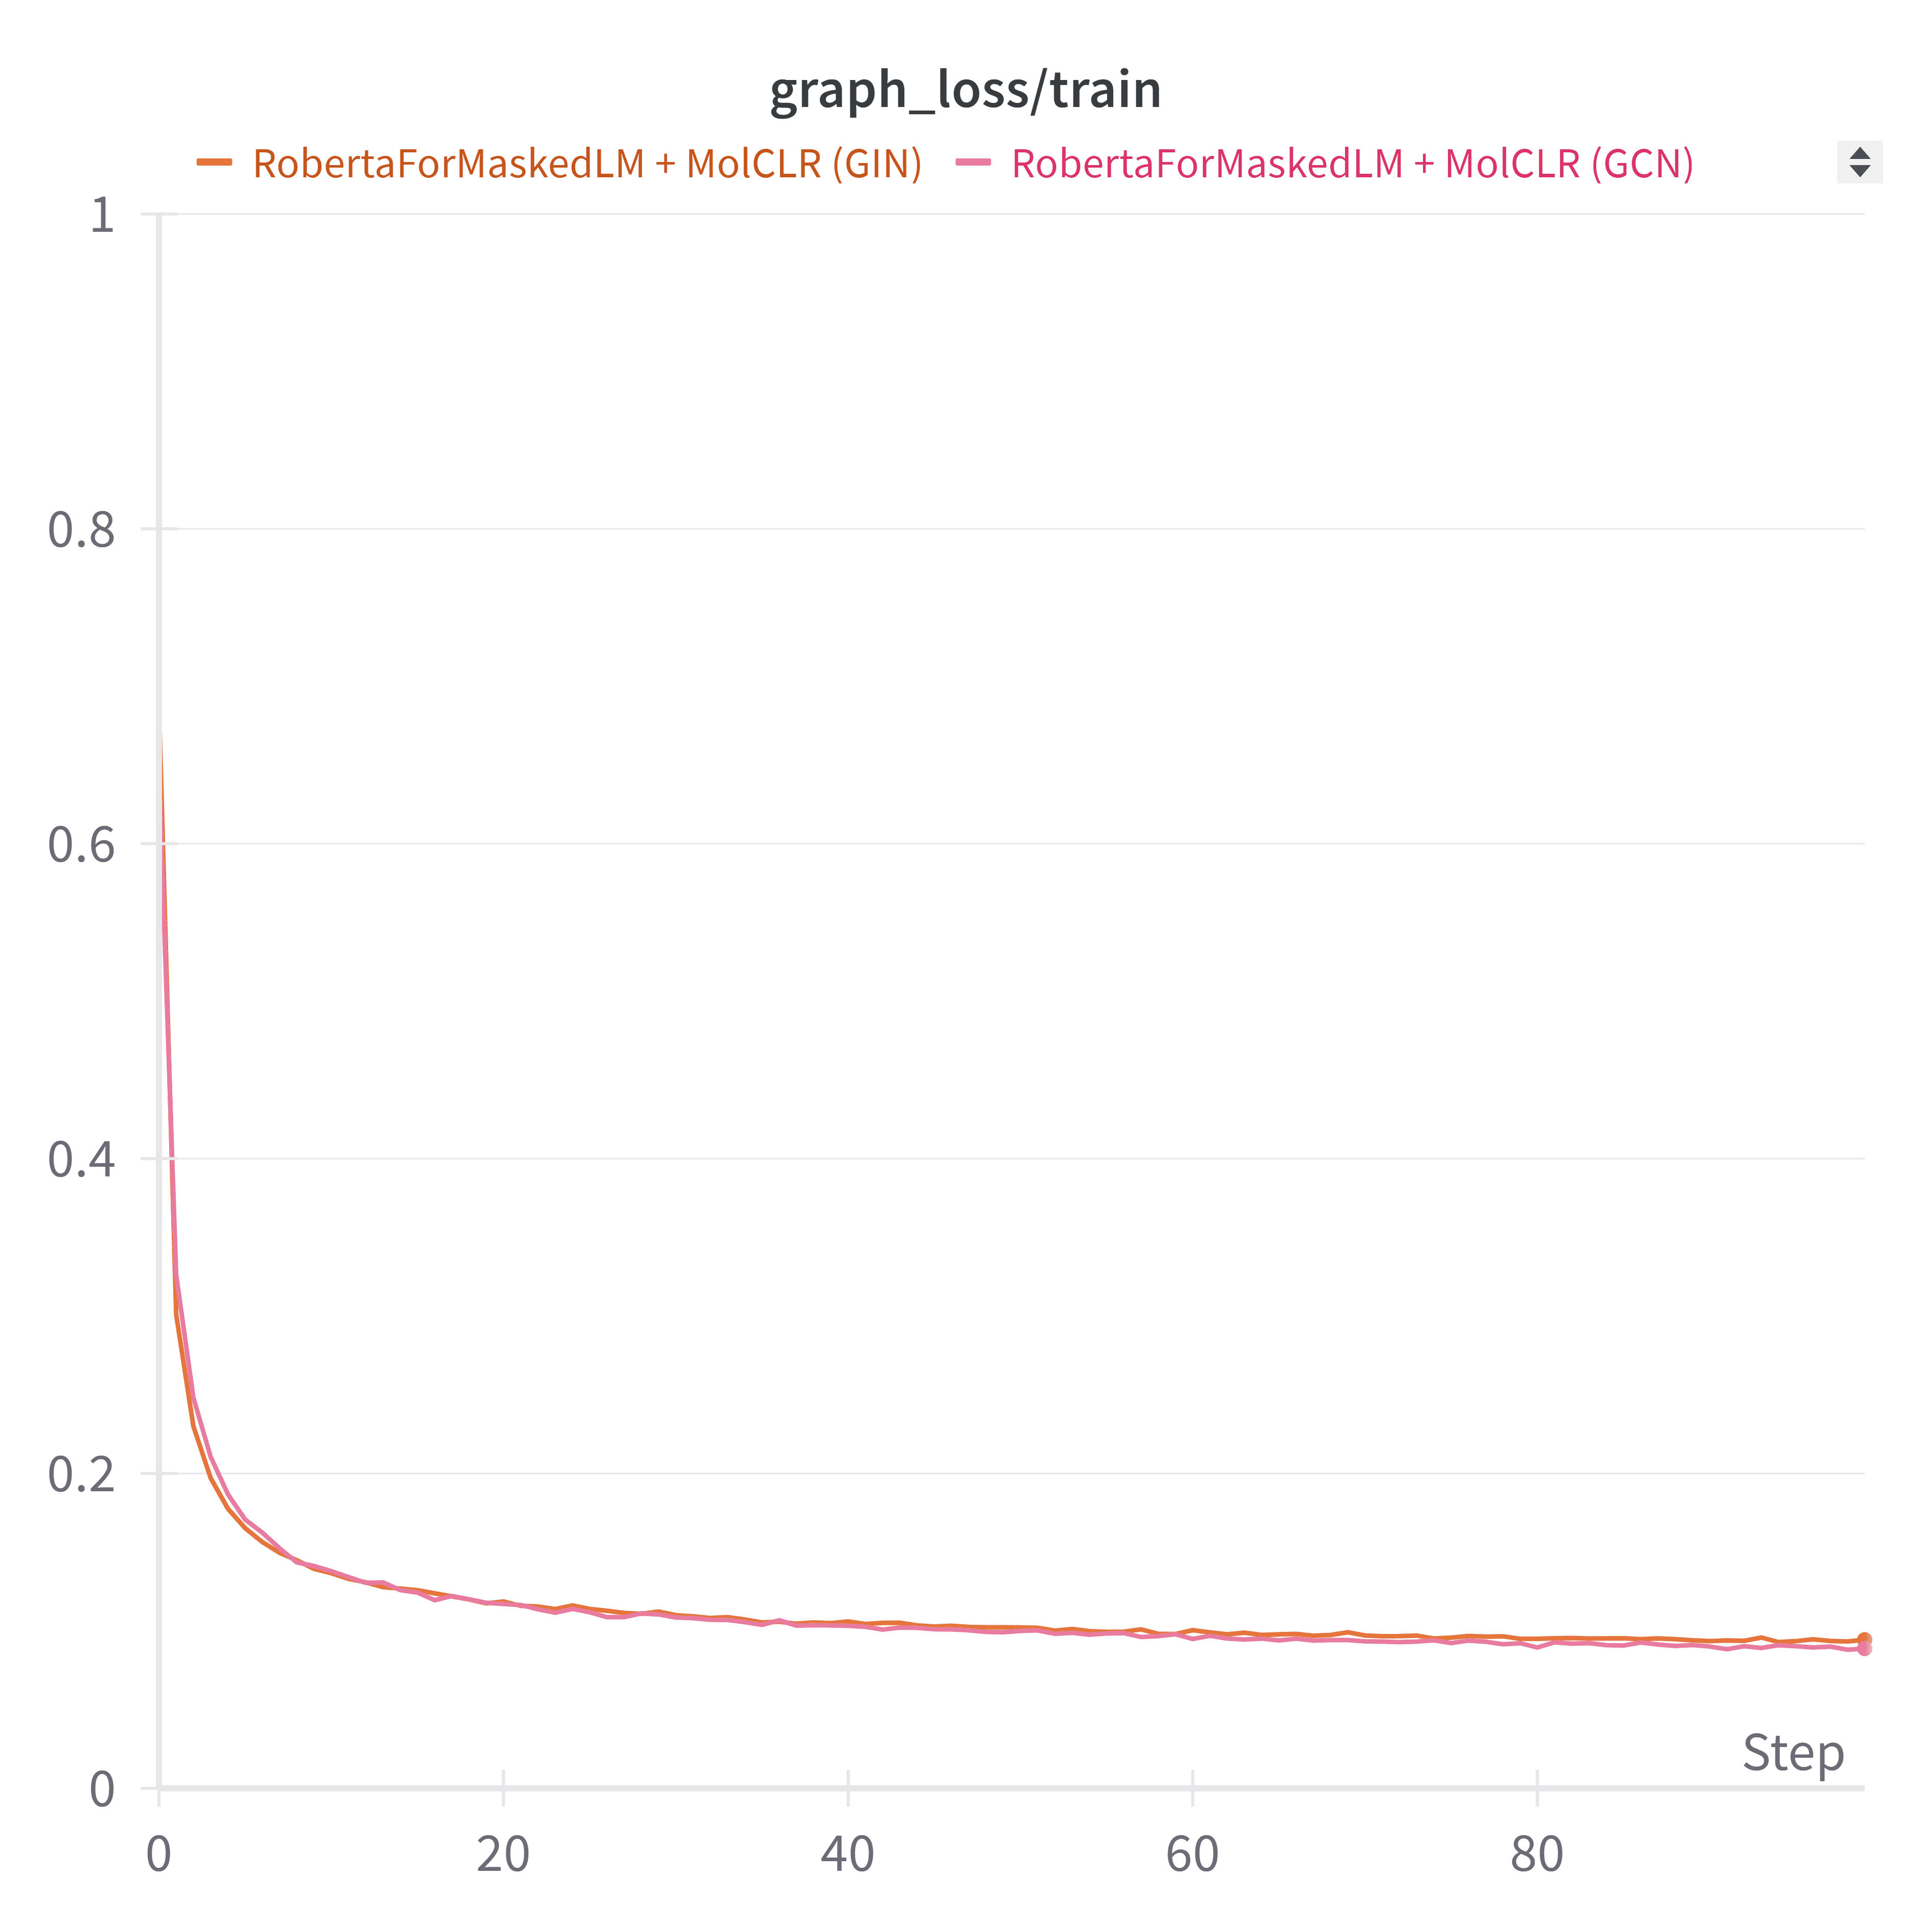
\includegraphics[width =  \textwidth ]{Bachelor-Thesis-Template/images/roberta_molclr/graph_loss_train.png}
    \end{minipage}%
    \begin{minipage}{0.5\textwidth}
        \centering
        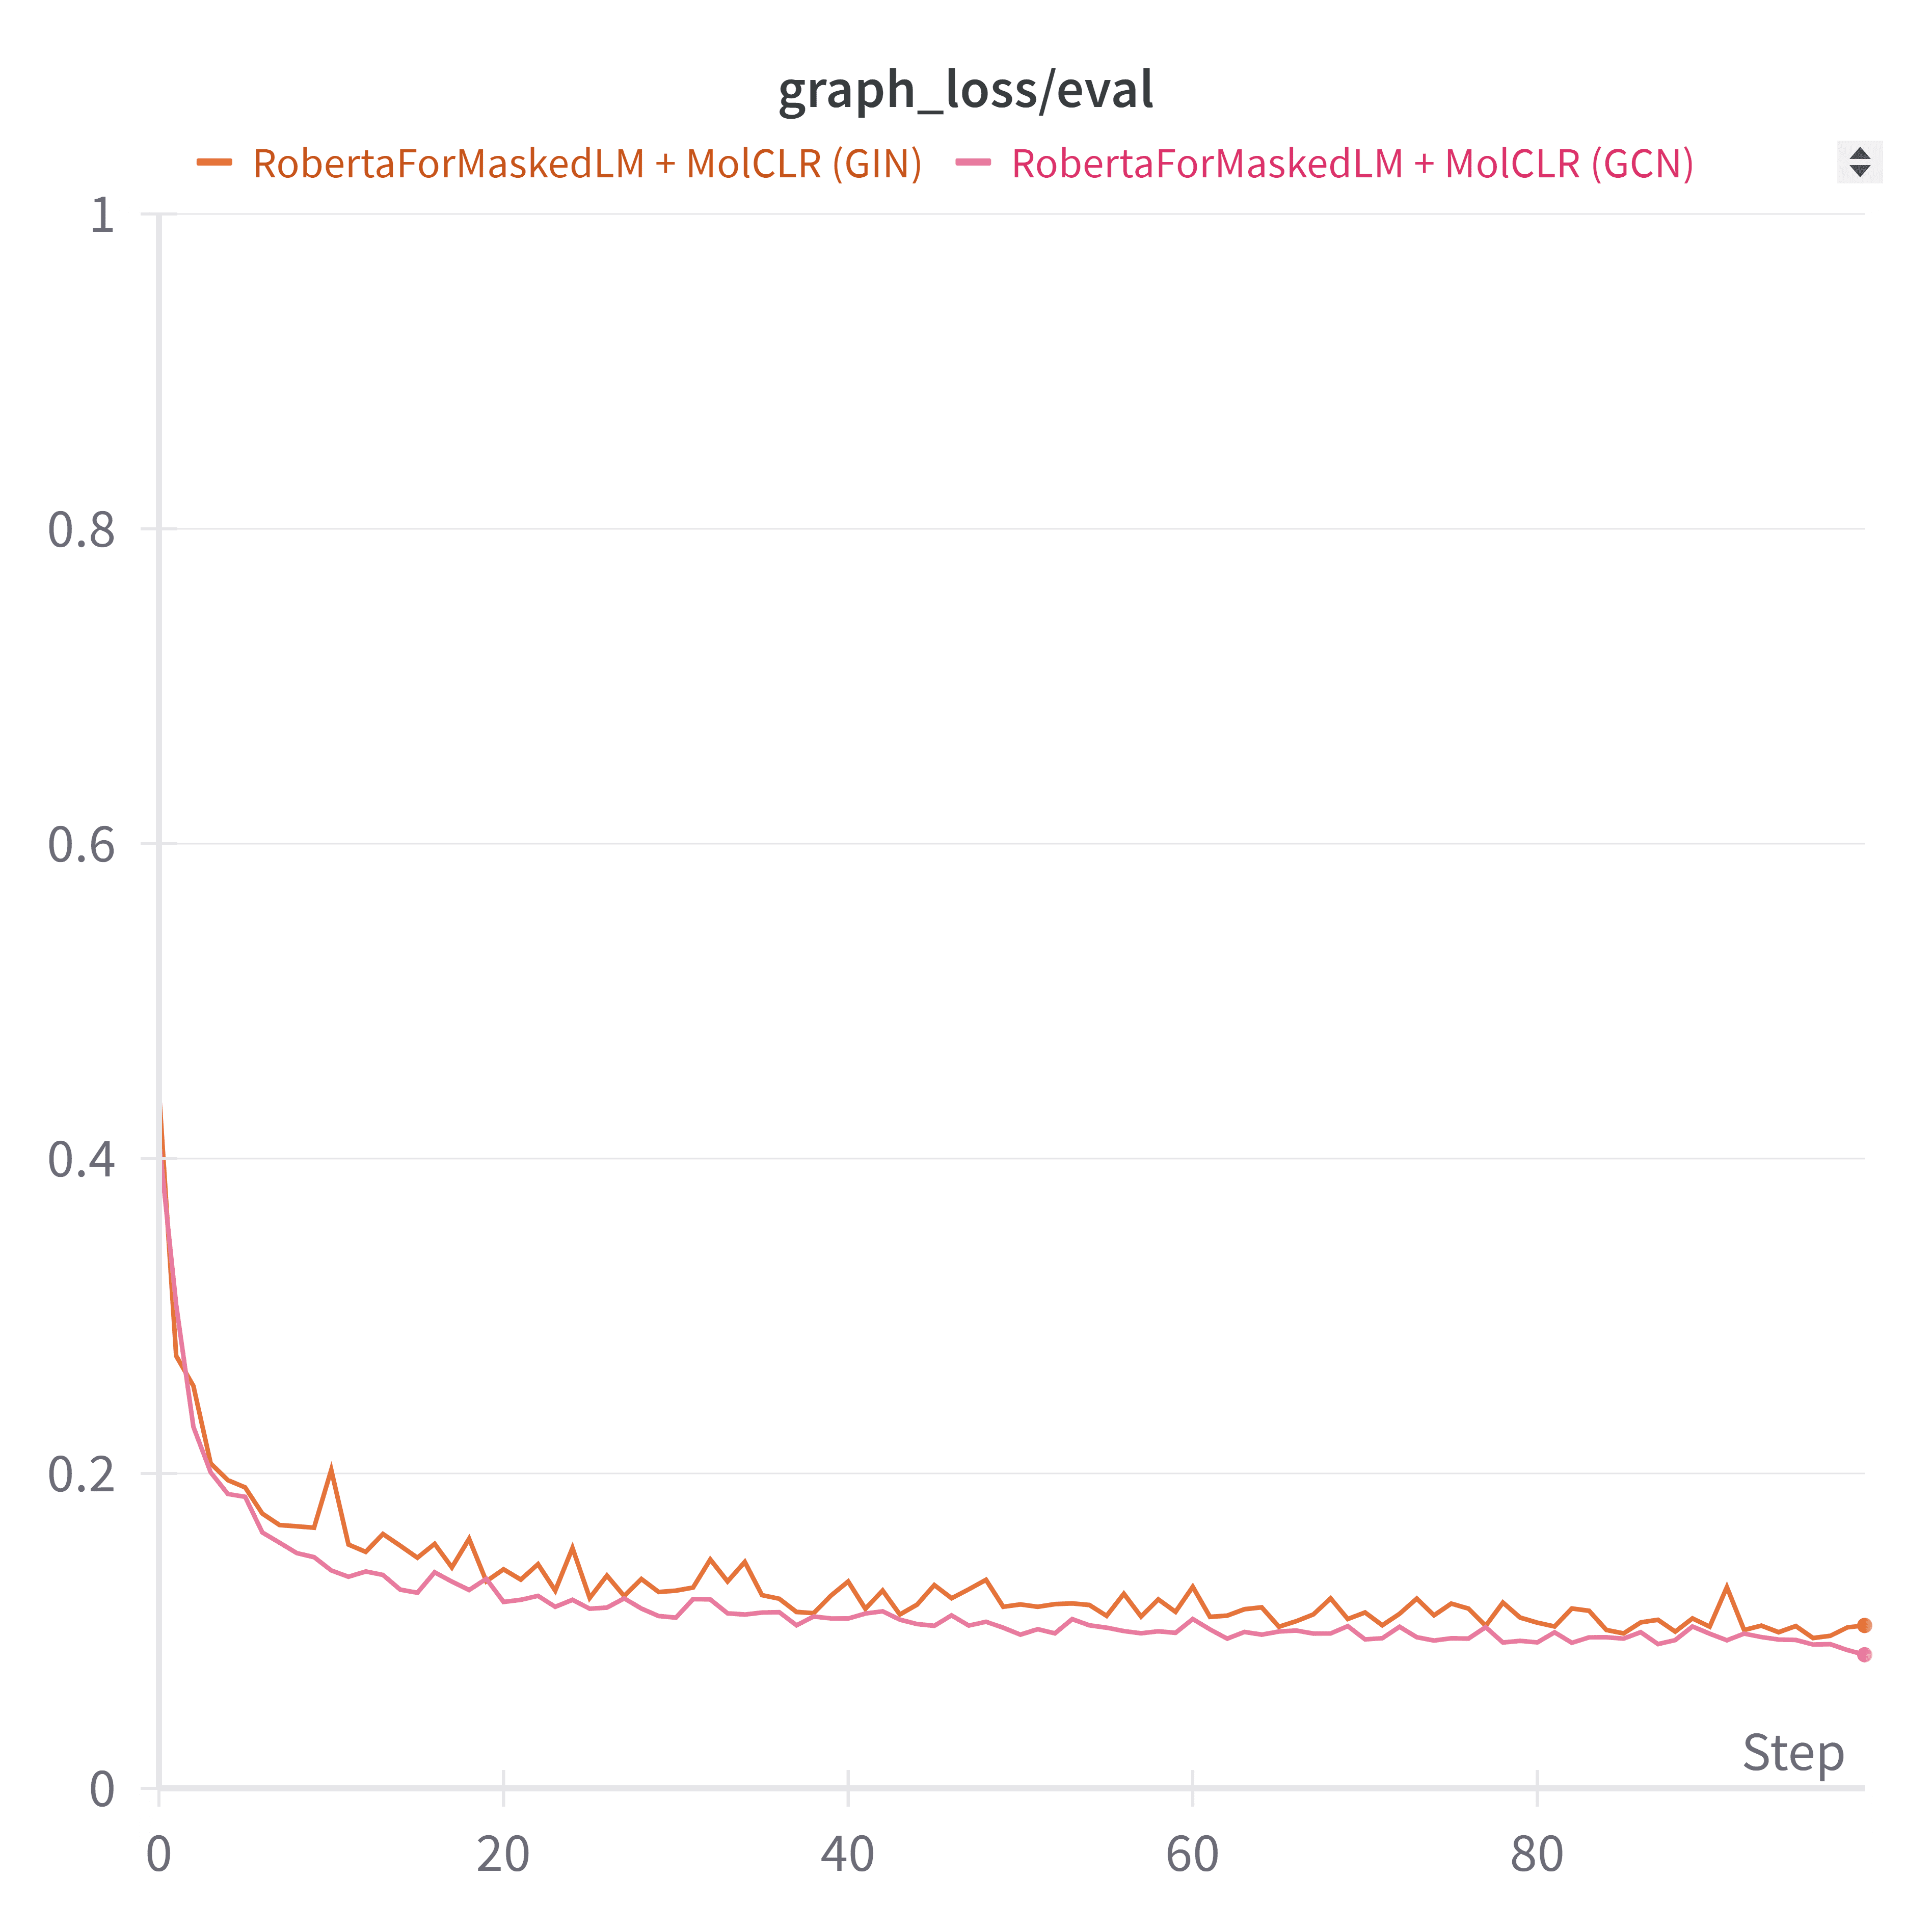
\includegraphics[width =  \textwidth ]{Bachelor-Thesis-Template/images/roberta_molclr/graph_loss_eval.png}
    \end{minipage}%

    \newline
    \begin{minipage}{0.5\textwidth}
      \centering
    \textbf{(a)}
    \end{minipage}%
    \begin{minipage}{0.5\textwidth}
    \centering
    \textbf{(b)}
    \end{minipage}%
    
    \caption{\small Графики функций потерь MolCLR в baseline-модели: (a) train, (b) validation}
    \label{fig:molclr_loss_bimodal}
\end{figure}
Функция потерь MolCLR также играет важную роль в общей функции потерь, поскольку она отражает эффективность модели MolCLR в генерации эмбеддингов графов молекул. Это подтверждается графиком \ref{fig:molclr_loss_bimodal}, где на обучении и валидации обе модели демонстрируют схожую динамику уменьшения функции потерь. Это указывает на то, что обе модели успешно обучаются, улучшают свою производительность с течением времени, однако быстро достигают "плато".

\begin{figure}[h]
    \begin{minipage}{0.5\textwidth}
        \centering
        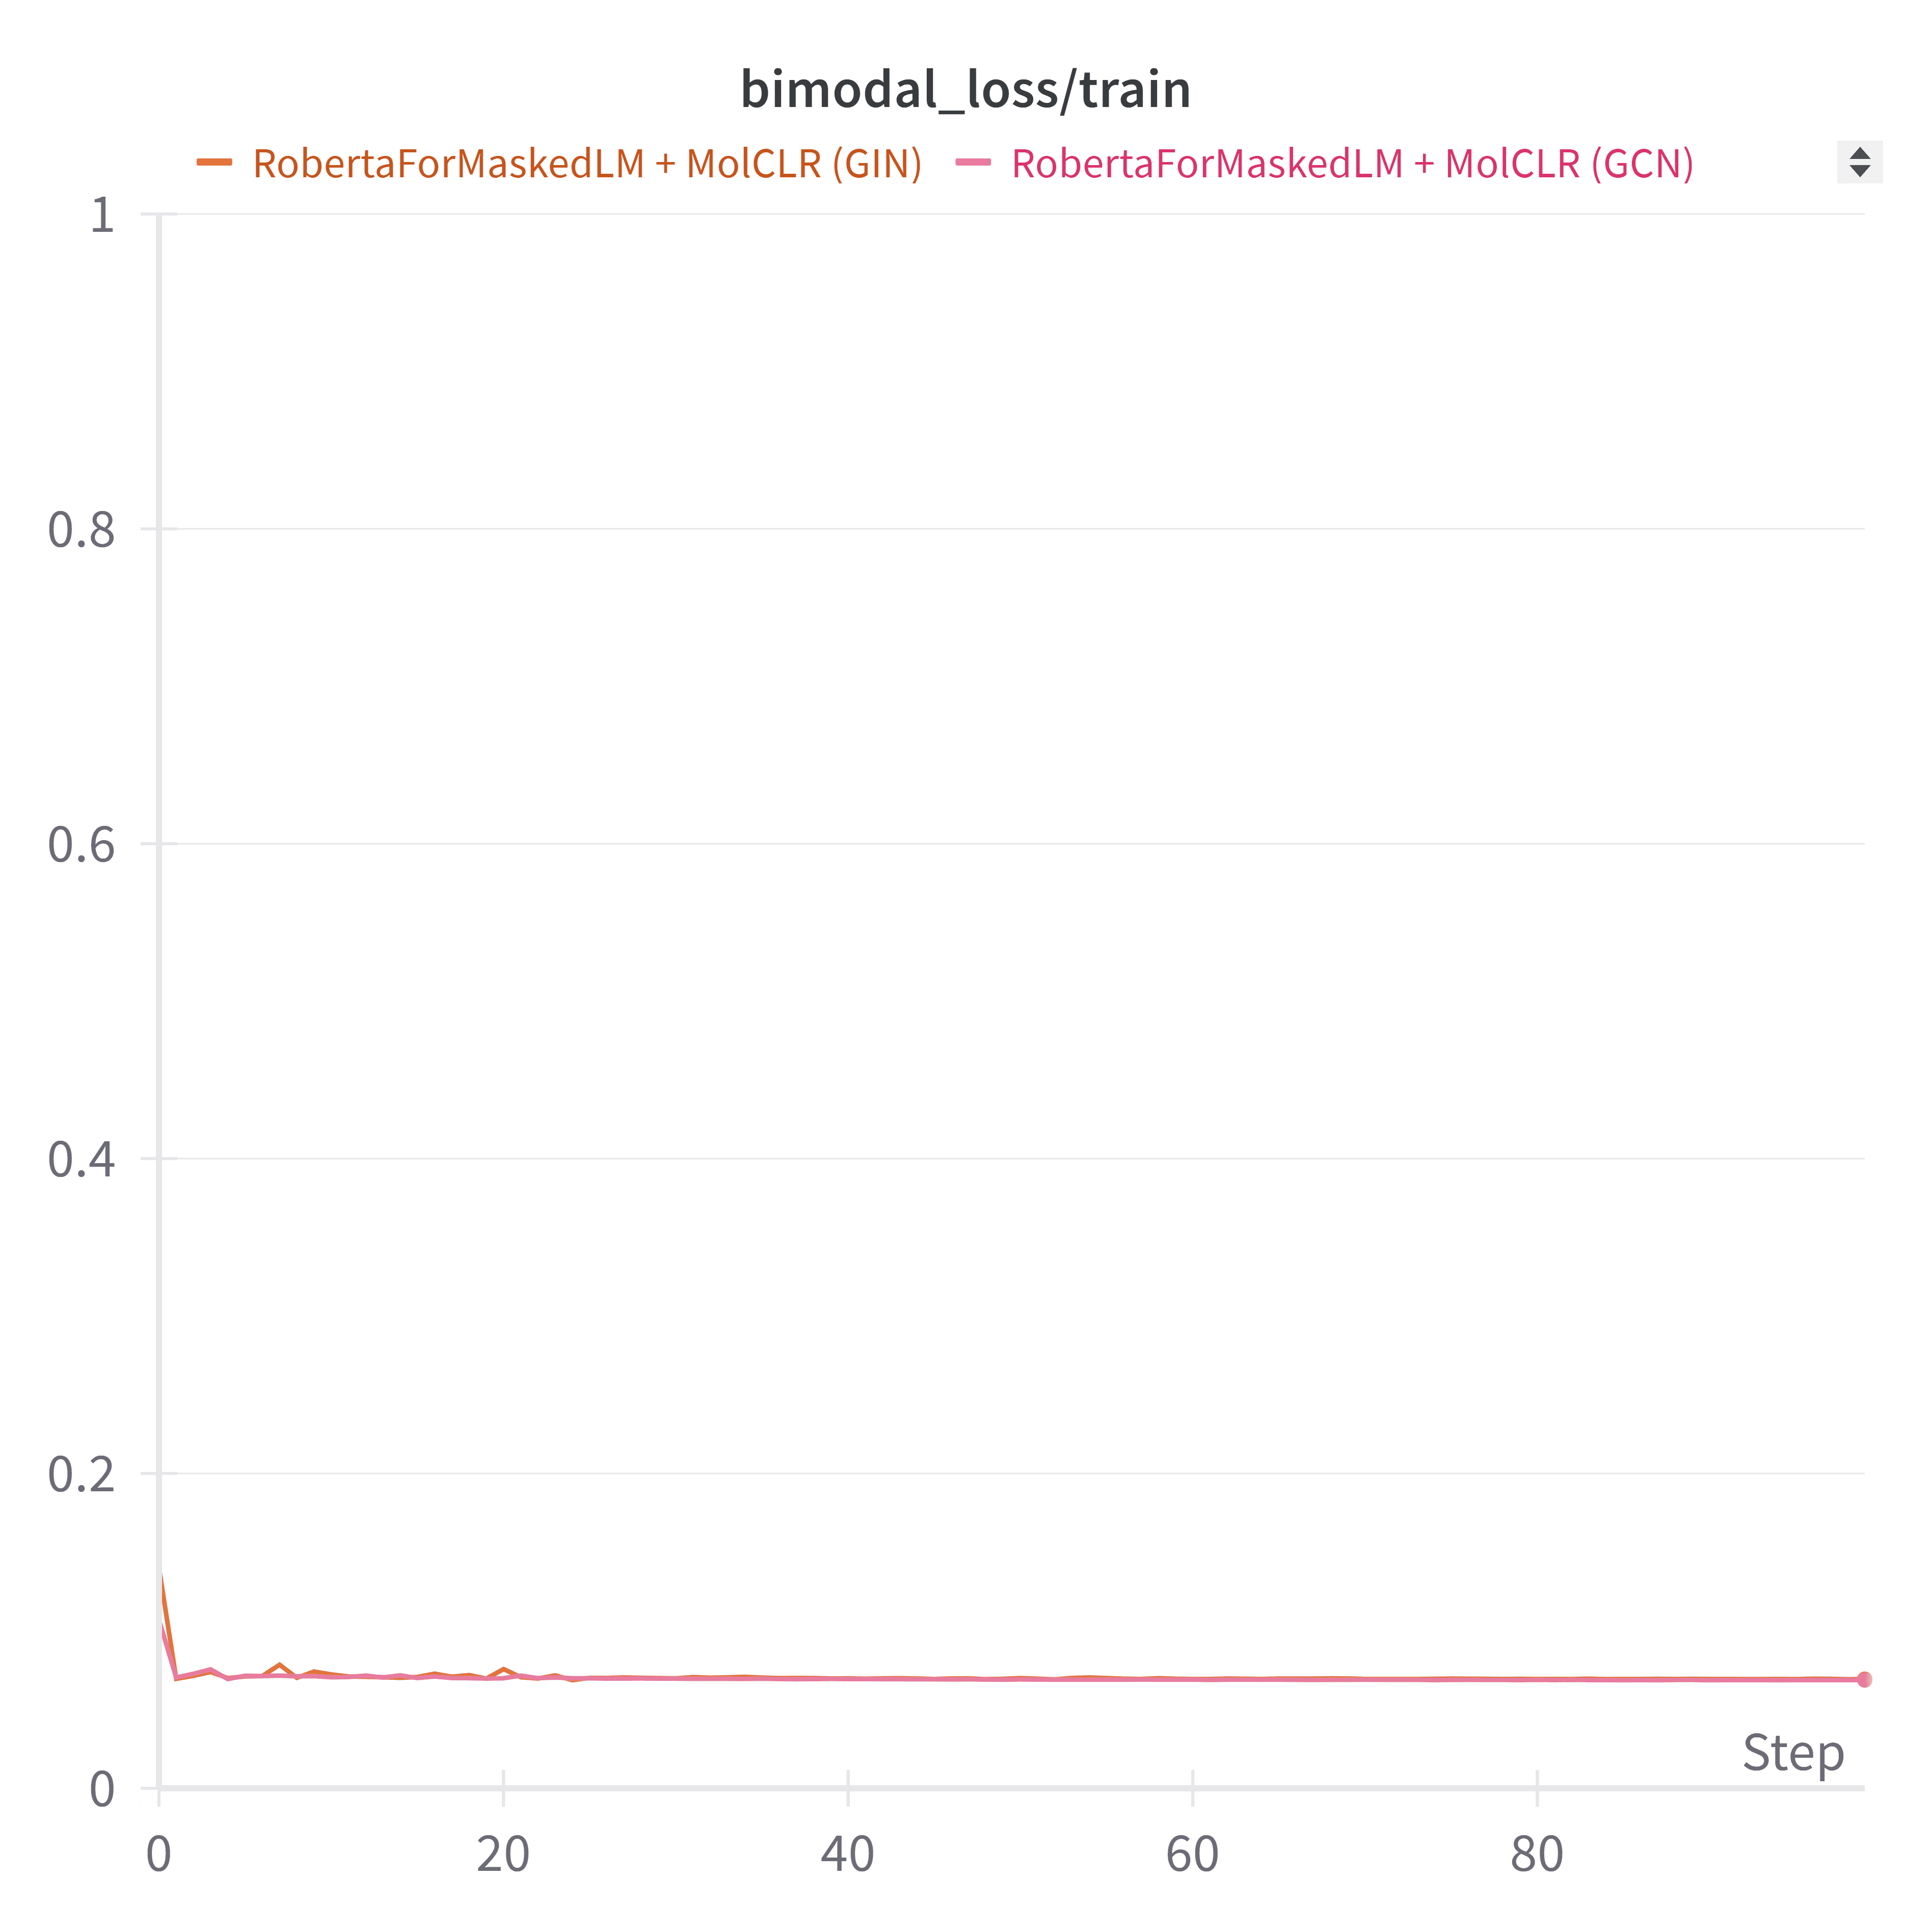
\includegraphics[width =  \textwidth ]{Bachelor-Thesis-Template/images/roberta_molclr/bimodal_loss_train.png}
    \end{minipage}%
    \begin{minipage}{0.5\textwidth}
        \centering
        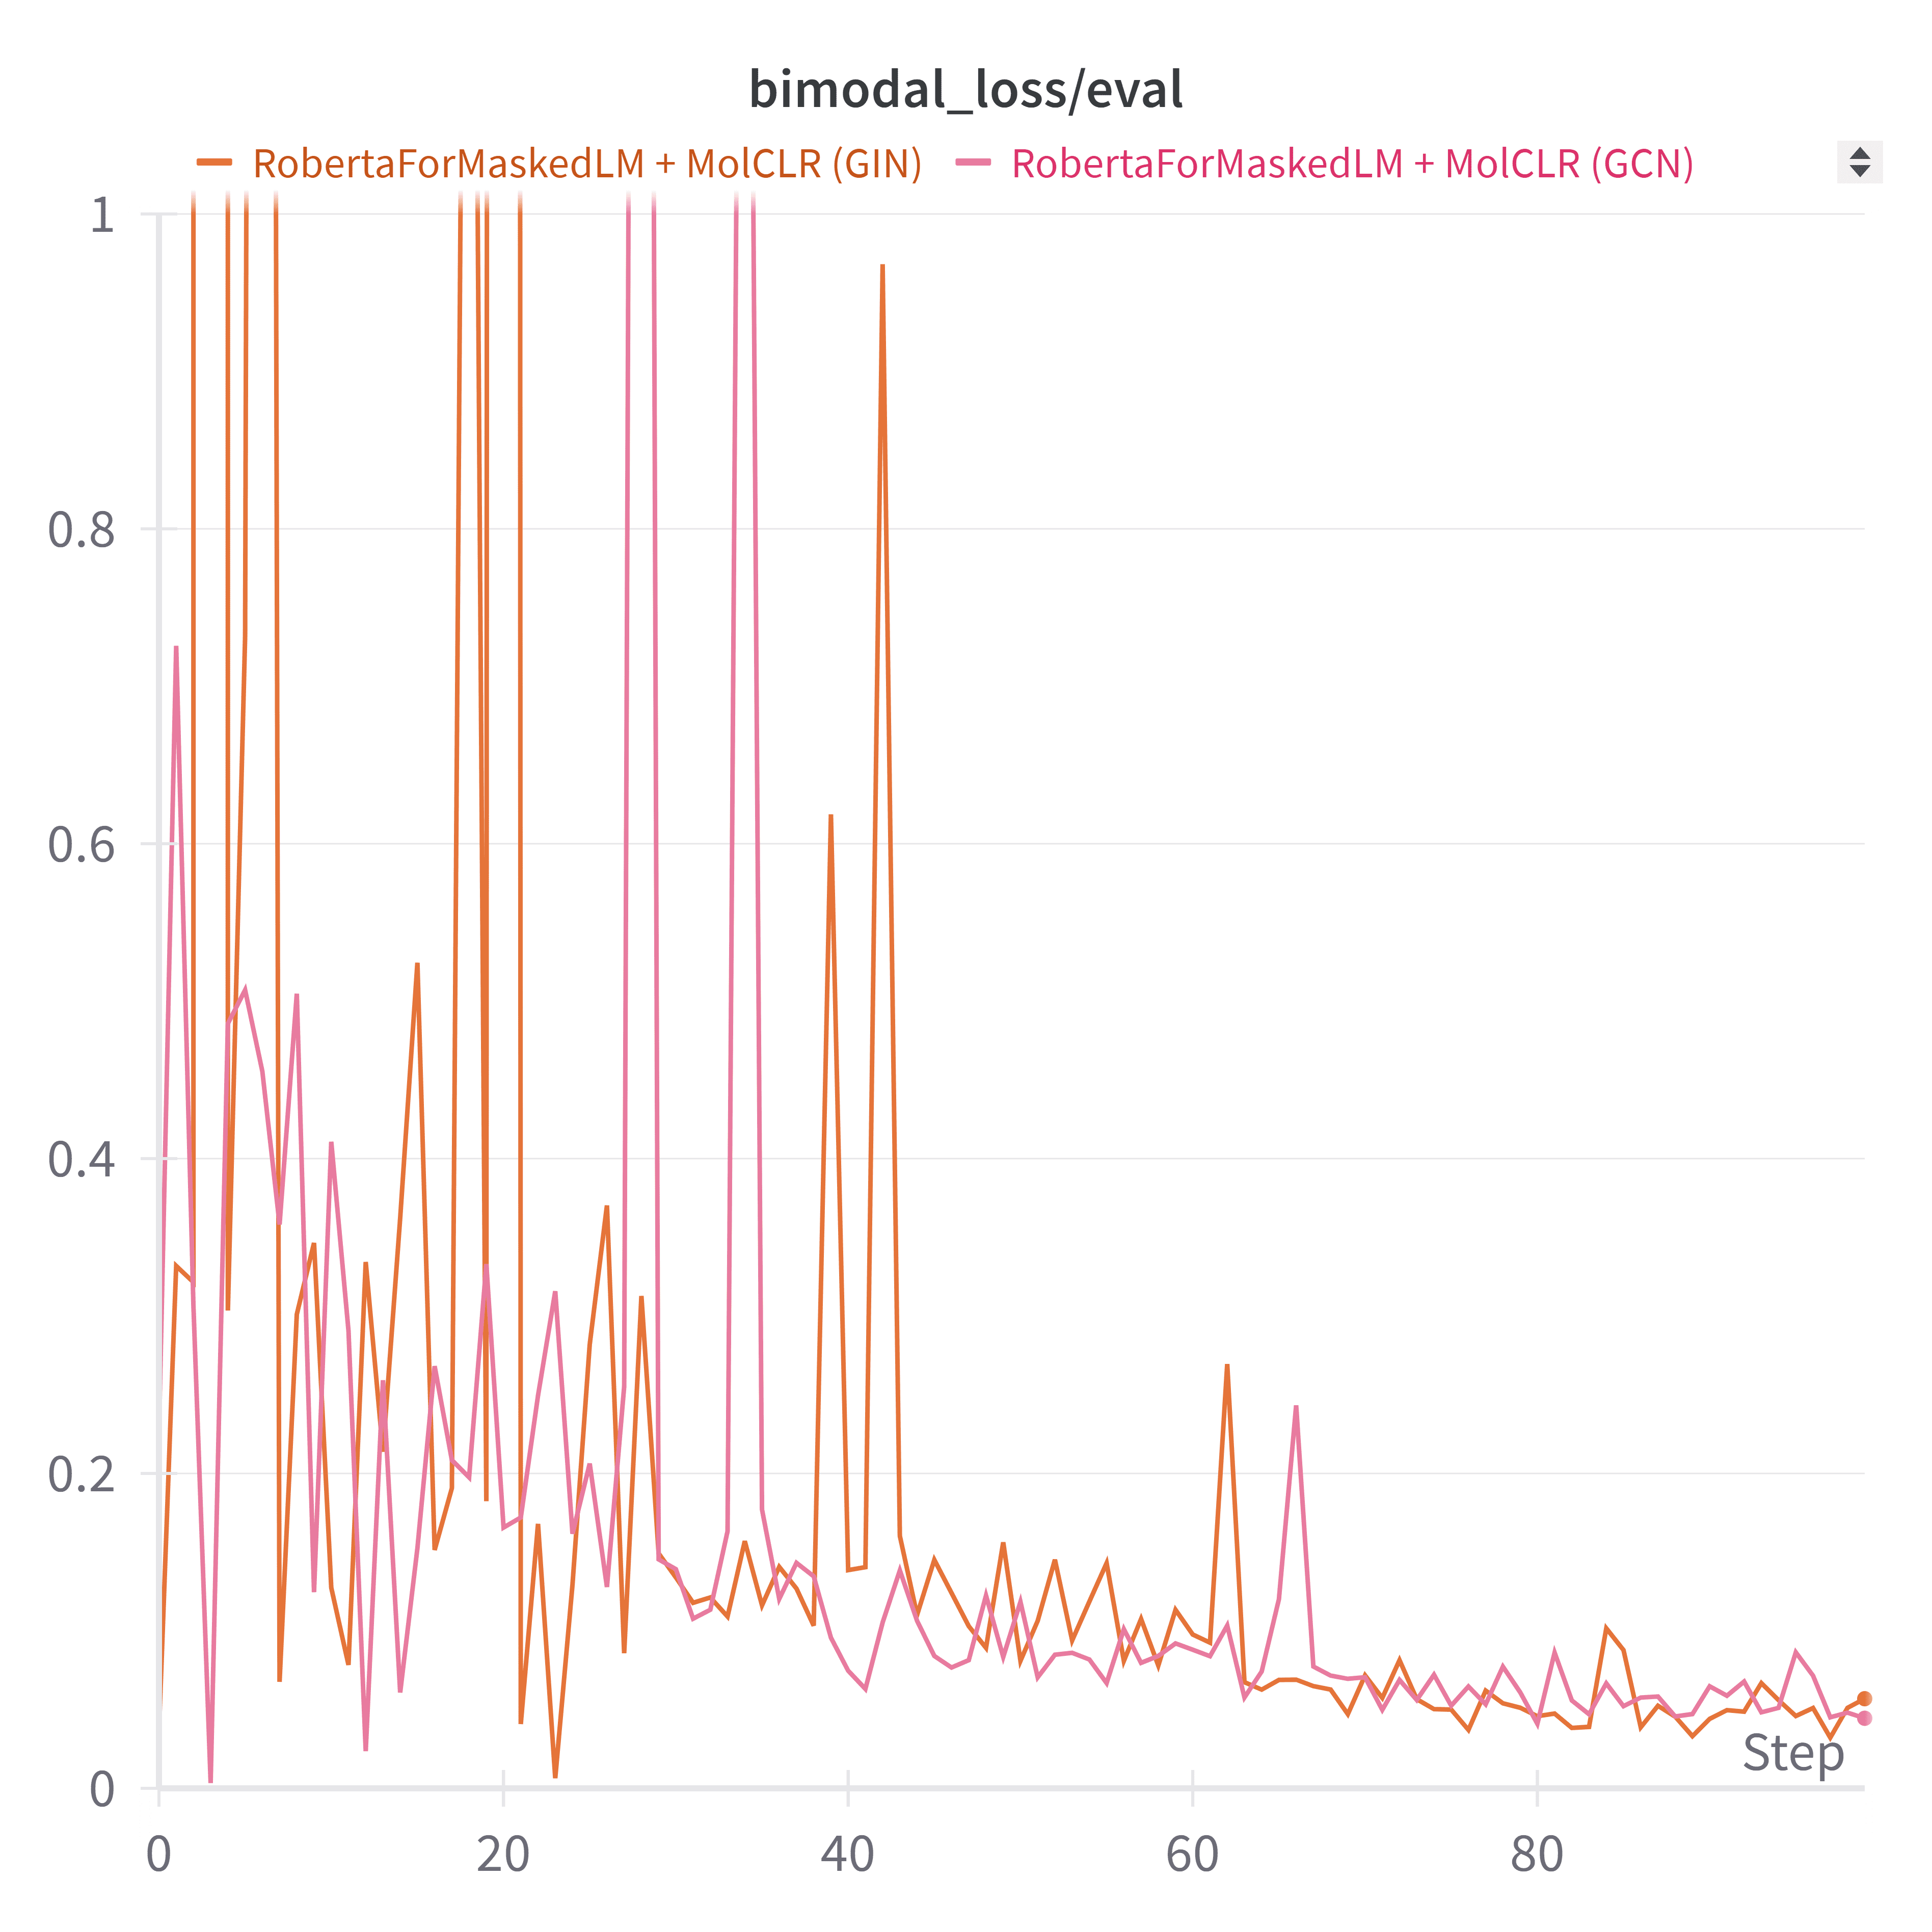
\includegraphics[width =  \textwidth ]{Bachelor-Thesis-Template/images/roberta_molclr/bimodal_loss_eval.png}
    \end{minipage}%

    \newline
    \begin{minipage}{0.5\textwidth}
      \centering
    \textbf{(a)}
    \end{minipage}%
    \begin{minipage}{0.5\textwidth}
    \centering
    \textbf{(b)}
    \end{minipage}%
    
    \caption{\small Графики бимодальной функций потерь в baseline-модели: (a) train, (b) validation}
    \label{fig:bimodal_loss_bimodal}
\end{figure}

На представленном выше графике рисунка \ref{fig:bimodal_loss_bimodal} отображены динамики бимодальной функции потерь на этапе обучени и валидации. Данная функция является косинусоидальным расстоянием между внутренними представлениями RoBERTa и MolCLR. Начальное значение (расстояние между случайными эмбеддингами) равно приблизительно 1, однако оно быстро сходится к числу, сильно меньше 0.1. Поэтому стоит отметить, что значения функции потерь на этом графике умножены на 100 для наглядности, поскольку исходные значения \texttt{bimodal\_loss} получаются слишком близкими к нулю.

Несмотря на то, что функция потерь между двумя моделями является важной составляющей общей функции потерь, ее вклад в общую функцию потерь оказывается относительно небольшим. Полученные результаты свидетельствует о высокой степени согласованности эмбеддингов, получаемых от моделей RoBERTa и MolCLR, а также достаточно быстрой сходимости данной функции похожести эмбеддингов при обучении.

\textbf{Про коэффиценты общего loss:}
В ходе экспериментов была предпринята попытка установить коэффициенты $\alpha$, $\beta$, $\gamma$ обратно пропорциональными начальным значениям соответствующих функций потерь. Однако, как показали результаты, такой подход приводит к эффекту, аналогичному случаю, когда все коэффициенты равны 1. Это может быть связано с тем, что обратная пропорциональность начальных значений потерь приводит к нормализации вклада каждой компоненты потери в общую потерю. В результате, каждая компонента потери вносит примерно одинаковый вклад в общую потерю.

Таким образом, для дальнейшего анализа были выбраны результаты, полученные при $\alpha = \beta = \gamma = 1.0$. В этом случае все функции потерь вносят одинаковый вклад в общую функцию потерь.



\newpage

 %% Описание практической части
    \section{Заключение}
\label{sec:Chapter5} \index{Chapter5}

В ходе выполнения данной дипломной работы была успешно решена задача исследования и применения методов обучения и fine-tuning для моделей машинного обучения молекулярных структур. Были достигнуты следующие ключевые результаты:
\begin{enumerate}
    \item Исследование уже существующих подходов к классификации и регрессии свойств молекулярных структур. Выбор наиболее успешных подходов, для последующей их проверки и применения (реализации) в решении задачи.
    \item Обучение и fine-tuning существующих моделей. Проведено обучение, валидация и тестирование моделей RoBERTa, Graphormer и MolCLR с использованием различных подходов к инициализации и настройке параметров. 
    \item Разработка и обучение новой модели. Обьединение существующие моделей RoBERTa и MolCLR, их совместное обучение и валидация. Результаты показали высокую степень согласованности эмбеддингов, получаемых от обеих моделей, а также высокое качество обучения данных моделей.
    \item Исследование новых подходов к классификации и регрессии. В процессе работы были изучены и протестированы новые методы классификации и регрессии молекулярных свойств. Применение трансформеров и графовых нейронных сетей позволило значительно повысить точность предсказаний по сравнению с традиционными методами.
\end{enumerate}

Настоящая работа вносит вклад в развитие методов машинного обучения для анализа и предсказания свойств химических соединений, открывая новые возможности для их практического применения.
\newpage
 %% Заключение

    %% НЕ ТРОГАЙТЕ!!!
    \nocite{*}
    \bibliography{references}

    %% в зависимости от надобности подключаем раздел "Приложение"
    % \newpage
    % \section*{Приложение}
\addcontentsline{toc}{section}{Приложение}
\label{sec:Apendix} \index{Apendix}

Здесь необходимо написать приложение, которое вы должны придумать самостоятельно.

\end{document}
